\chapter{Magnetic field Morphology of the Carina Nebula Complex}\label{carina}

In the following sections, we describe the preliminary data reduction and analysis of BLASTPol 2012 \citep{galitzki2014balloon} observations of the Carina Nebula Complex (NGC 3372, hereafter CNC). These BLASTPol maps have the highest spatial resolution of any polarized sub-mm map of the CNC to date ($\sim$2.5$\arcmin$). Recently, \citet{shariff2015polarimetry} used the same data set to produce the CNC's dust polarization spectrum. The authors calculated the polarization ratio $p_\lambda/p_{350\upmu m}$ along 314 sightlines, and found it to be flat within $\pm 15\%$ over the three BLASTPol wavebands (250, 350 and 500~$\upmu$m). While the flatness of the spectrum agrees with other BLASTPol observations of molecular clouds (MCs) (e.g., \citet{ashton2018first,gandilo2016submillimeter}), it is in stark contrast to existing sub-mm/FIR polarization spectra of MCs (see, e.g., \citet{vaillancourt2012submillimeter}), which show V-shaped spectra with a negative slope towards the FIR, a positive slope towards the millimeter, and minima near 350~$\upmu$m.

The goal of the data analysis presented in this work is to describe the morphology of the magnetic field (B-field) in the plane-of-the-sky (POS) \gls{Bpos} in the CNC as revealed by the BLASTPol data, compare it to previous observations, and to provide what are possibly the first estimates of the magnitude of \gls{Bpos} along various sightlines through the cloud. To aid in visualizing the field, we apply a vector field visualization technique called line-integral-convolution (LIC). This chapter is organized as follows:

\begin{itemize}[nosep]
  \item Section~\ref{observations} introduces the BLASTPol CNC map and describes its acquisition and calibration.
  \item Section~\ref{LIC} presents an original software implementation of the LIC algorithm.
  \item In Section~\ref{multiband comp}, we compare the BLASTPol CNC to maps made in different wavebands in order to investigate how the dust component of the cloud relates to other sources of emission.
  \item In Section~\ref{DCFM}, we apply the Davis-Chandrasekhar-Fermi Method (DCFM) to the CNC map and present estimates of \gls{Bpos} along several sightlines of interest.
\end{itemize}

\section{BLASTPol Observations of Carina}\label{observations}
The BLASTPol telescope (\citet{galitzki2014balloon}) launched from McMurdo Station, Antarctica, during the summer 2012/2013 season, and observed several targets over the course of $\sim$12.5 days. Its camera incorporated 139, 88 and 43 pixels in 30$\%$ bands centered at 250~$\upmu$m, 350~$\upmu$m and 500~$\upmu$m. The detectors were superconducting spiderweb bolometers (SWBs) based on those used in Herschel SPIRE \citep{griffin2003spire}.
The BLASTPol telescope had a 1.8~m primary mirror, which provided nominal diffraction limited resolutions in the three bands of 30$\arcsec$, 42$\arcsec$ and 60$\arcsec$. However, deformations in the telescope optics introduced a non-Gaussianity to the point spread function (PSF) (see \citet{fissel2016balloon}). After correcting for the warped PSF, the resulting resolution of the maps is $\sim$2.5$\arcmin$.

BLASTPol observed the CNC for 4.2 hours, and the resulting map is $\sim$2.5~deg$^{2}$ in area. The target coverage was chosen to overlap with previous observations taken at 450~$\upmu$m by the Submillimeter Polarimeter for Antarctic Remote Observations (SPARO, \citep{li2006results}). As discussed in \citet{benton2015mapping}, the detector timestreams taken during the CNC mapping were contaminated by interference from the Tracking and Data Relay Satellite System (TDRSS) traffic. The loss of data made it difficult for the map maker to converge to a solution, and some artifacts are present in the resulting maps. The maps were created with the Time-Ordered Astrophysics Scalable Tools (TOAST)\footnote{\url{https://github.com/tskisner/TOAST}} package. TOAST produces a (3 $\times$ 3) $I$, $Q$, $U$ covariance matrix for each pixel (where $I$, $Q$, and $U$ are the Stokes parameters). Raw analog-to-digital-converter (ADC) detector counts were calibrated into beam-averaged flux density ($\mathrm{MJy}/\mathrm{sr}$) using the Planck all-sky thermal dust model \citep{ade2015planck}.

\subsection{Data parameterization}

The map for each BLASTPol band are parameterized in terms of the first three Stokes Parameters, $I$, $Q$ and $U$. The Stokes parameters describe the polarization state of measured light. In this work, they have been calibrated into units of $\mathrm{MJy}/\mathrm{sr}$. Each Stokes parameter can be written as either the sum or the difference between the squared magnitudes of electric field (E-field) vectors which are oriented along different axes of a Cartesian coordinate system (for a detailed description of the Stokes parameters, see \citet{hecht2002optics}). The coordinate system can be parameterized in terms of Jones Vectors, which form three orthogonal bases: $x$ and $y$, $a$ and $b$ (rotated 45$^{\degree}$ with respect to the $x-y$ plane), $l$ and $r$ ($\hat{l} = (\hat{x} + j\hat{y})/\sqrt{2}$, $\hat{r} = (\hat{x} - j\hat{y})/\sqrt{2}$).

Using these bases, the Stokes parameters can be written as:

\begin{equation}
  \begin{split}
  I &= \langle \lvert E_{x} \rvert ^{2} \rangle + \langle \lvert E_{y} \rvert ^{2} \rangle = \langle \lvert E_{a} \rvert ^{2} \rangle + \langle \lvert E_{b} \rvert ^{2} \rangle = \langle \lvert E_{l} \rvert ^{2} \rangle + \langle \lvert E_{r} \rvert ^{2} \rangle \\
  Q &= \langle \lvert E_{x} \rvert ^{2} \rangle - \langle \lvert E_{y} \rvert ^{2} \rangle \\
  U &= 2\langle \Re \left( E_{x}E_{y}^{\star} \right) \rangle = \langle \lvert E_{a} \rvert ^{2} \rangle - \langle \lvert E_{b} \rvert ^{2} \rangle \\
  V &= -2\langle \Im \left( E_{x}E_{y}^{\star} \right) \rangle = \langle \lvert E_{l} \rvert ^{2} \rangle - \langle \lvert E_{r} \rvert ^{2} \rangle
  \end{split}
\end{equation}

where $V = 0$ in the case of linearly polarized light, and the inequality becomes an equality in the case of circularly polarized light. The parameters are related as:

\begin{equation}
  \lvert I \rvert ^{2} \geq \lvert Q \rvert ^{2} + \lvert U \rvert ^{2} + \lvert V \rvert ^{2}
\end{equation}

with:

\begin{equation}
  Q + jU = Pe^{j2\Psi} = p I e^{j2\Psi}
\end{equation}

where $P = \sqrt{Q + U}$ is the total intensity of linearly polarized light, and \gls{Psi} is the polarization angle

\begin{equation}\label{eq:pol angle}
  \Psi = \frac{1}{2} \arctantwo(U, Q)
\end{equation}

where $-90^{\degree} \leq \Psi \leq 90^{\degree}$. In this work we use the astronomical polarization angle convention, where $\Phi$ increases counter-clockwise from the north \citep{shariff2015polarimetry}. The inferred angle of \gls{Bpos} is $\Phi = \Psi + 90^{\degree}$.

The polarization fraction is defined as:

\begin{equation}\label{pol frac}
  p = \frac{\sqrt{Q + U}}{I} = \frac{P}{I}
\end{equation}

\subsection{Data Calibration}\label{data_cal}

In this work, the resolution of the CNC Stokes maps are smoothed to 5$\arcmin$ full-width-half-max (FWHM) to match that of the 353~GHz (850~$\upmu$m) Planck maps. This is done so that the Planck and Carina data can be combined to produce estimates of \gls{Bpos} using the DCFM (see Section~\ref{DCFM}). The smoothing is performed using Lucy-Richardson iterative deconvolution (\citet{lucy1974iterative,richardson1972bayesian}). After smoothing, the steps taken to further clean the data are similar to those described in \citet{shariff2015polarimetry}. First, a background subtraction is applied to the map data. This is done to remove the brightness contribution from the diffuse Galactic background. The background subtraction is performed by first selecting a region near the edge of the map, where the average flux density is close to the minimum of the map. The average flux density in this region is then subtracted from each map pixel.

After background subtraction, the polarization fraction values $p$ are debiased. The debiased polarization fraction $p_{db}$ is calculated as:

\begin{equation}
  p_{db} = \sqrt{p^{2} - \sigma_{p}^{2}}
\end{equation}

where the variance in $p$ is calculated using the covariance maps and standard error propagation techniques. Following the debias, a 2$\sigma$ cutoff is applied to $p$, and all pixels containing $p > 0.5$ are eliminated from the map. Finally, the polarization fractions for each of the three observation bands are divided by their respective polarization efficiencies (0.81, 0.79 and 0.82, for 250, 350 and 500~$\upmu$m). Figure~\ref{fig:I250} shows the background-subtracted $I_{250}$ map, with regions of interest (ROI) outlined in green. The regions are listed in Table~\ref{table:regions}, and discussed in Section~\ref{multiband comp}. A detailed analysis of the polarization fraction over the inner region of the CNC is found in \citet{shariff2019submillimeter}.

In the following analysis, all calculations use the debiased polarization fraction and polarization angle (see Section~\ref{LIC}).

\begin{figure}[!htbp]
\centering
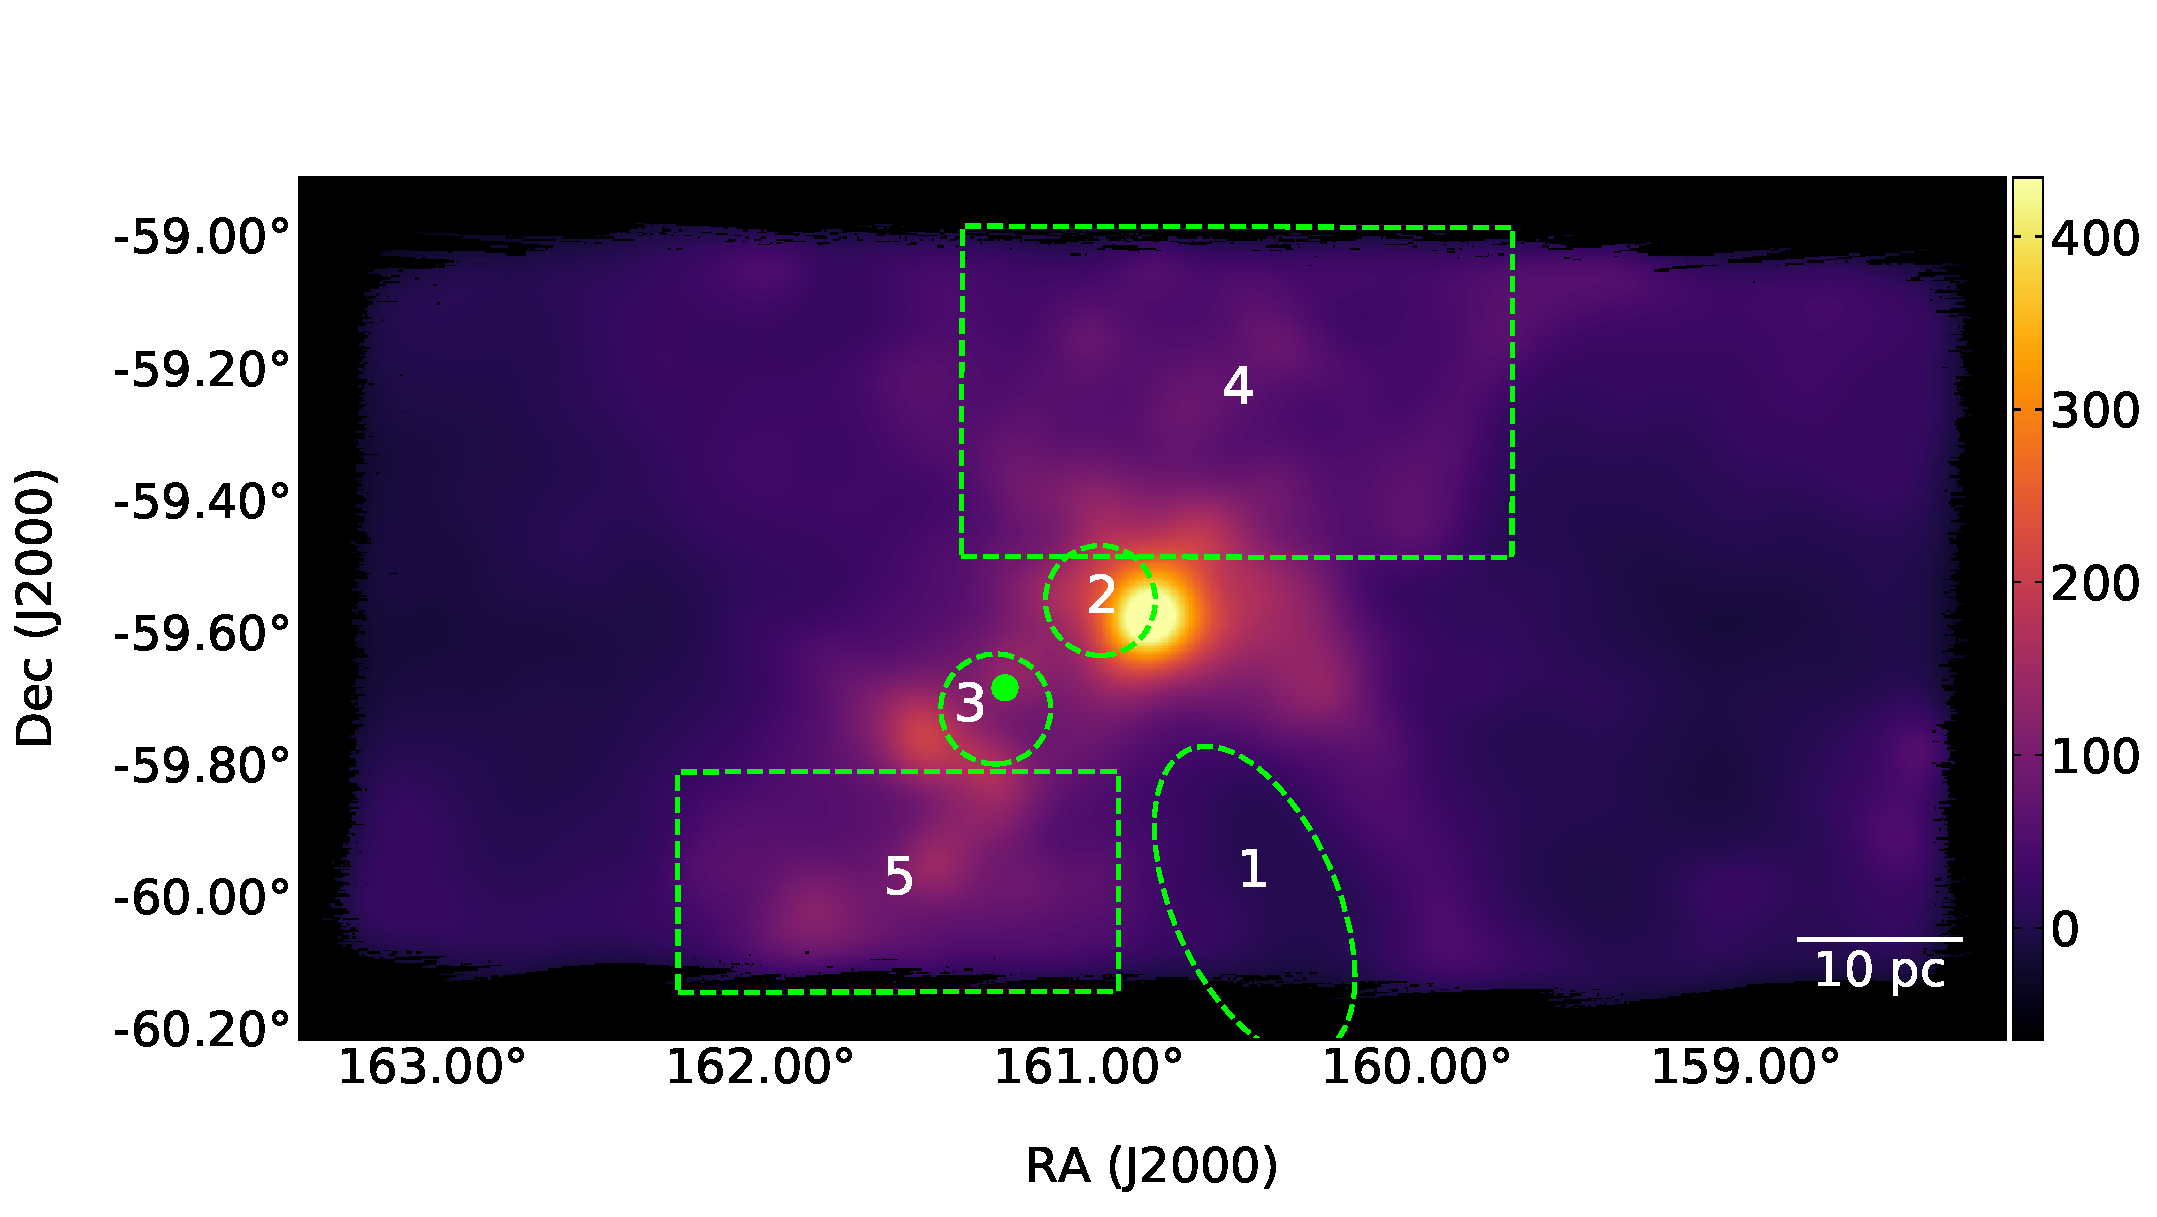
\includegraphics[width=\textwidth]{figures/carina/carina_I250}
\caption[The background-subtracted BLASTPol 2012 \macrocapwrap{$I_{250}$} map of the CNC.]{The background-subtracted BLASTPol 2012 $I_{250}$ map of the CNC\@. The color scale has units of $\mathrm{MJy}/\mathrm{sr}$.}
\label{fig:I250}
\end{figure}

\section{Line-Integral-Convolution}\label{LIC}

LIC is a data visualization technique which is useful for representing dense vector fields, in either two or three dimensions \citep{cabral1993imaging}. The visual effect that it produces is akin to that of dropping ink into flowing water. The resulting images provide a visual sense of the direction and uniformity of the vector field, allowing the eye to notice features such as sources, sinks and loops. The LIC does not, however, indicate the magnitude of the vector field.

The LIC technique has previously been applied to maps of \gls{Bpos} (see, e.g., \citet{ade2016planck}). In the following, we present an original software implementation of LIC which has been written in \texttt{C/Python}. Although fast, computationally efficient algorithms for LIC exist, the main priorities for this particular implementation were simplicity and flexibility. To that end, the basic skeleton of the code is based on a bare bones LIC algorithm, which is described in \citet{ma1996texture}.

To create a LIC image requires two basic ingredients: A vector (or pseudovector) field $\boldsymbol{\mathcal{V}}$, and a texture map $\mathcal{T}$, each of size $N \times N$ pixels. In the following example, we use the polarization vector field for Carina, and a texture map consisting of Gaussian white noise. The value of the \textit{ith} pixel in the polarization vector map is a pseudovector whose magnitude is the polarization fraction $p_{i}$:

\begin{equation}\label{eq:pol vector}
  \boldsymbol{v}_{i} = \left< \mathrm{\cos}(\Psi_{i}), \mathrm{\sin}(
  \Psi_{i}) \right>
\end{equation}

where the polarization angle $\Psi_{i}$ is calculated as:

\begin{equation}\label{eq:pol angle 2}
  \Psi_{i} = \frac{1}{2}\arctantwo(U_{i}, Q_{i})
\end{equation}

The method of LIC is to advect a streamline from each pixel which follows the direction indicated by that pixel's pseudovector (both positive and negative directions) into the adjacent pixels. This process continues until the streamline is terminated by one of several end conditions. The resulting streamlines, when downsampled by some factor, are also useful for map analysis. After the streamlines are created, the values of $\mathcal{T}$ which underly the streamline segments in each pixel are convolved with a filter kernel. These steps are described in more detail in the the following sections.

\subsection{LIC Algorithm}

The first step in creating an LIC image is to launch, or advect, a streamline $\sigma(s)$ from each pixel in the map image, $\mathcal{M}$. At any point in $\mathcal{M}$, the direction of the streamline is tangent to the vector at that point: $\frac{ d\boldsymbol{\sigma(s)}}{ds} = \boldsymbol{ \frac{ v(\sigma(s)) }{\lvert v(\sigma(s)) \rvert} }$. The entire vector field for the CNC is shown in Figures~\ref{fig:vectors_5} and~\ref{fig:vectors_10}, where the vectors have been rotated by 90$^{\degree}$ to correspond to the direction of \gls{Bpos}, and decimated by a factors of 5$\times$ and 10$\times$, respectively. The streamlines extend forwards and backwards along their starting vectors, into each adjacent pixel. This process continues until it is terminated by a break condition.

One common break condition is when a streamline enters into a pixel containing a null vector. In this case, the streamline may simply be terminated, or some non-zero value may be substituted for the null vector in order to attempt to continue the streamline. Another common break condition is when a streamline encounters the edge of the map. Discontinuities occur when a streamline enters an adjacent pixel whose vector forms an angle with the first one which exceeds some critical value (e.g., in the range of of 120--180$^{\degree}$). There are several ways of dealing with each case, each of which results in a slightly different LIC image.

In the CNC code, streamline advection is achieved using Eulerian advection, as in \citet{cabral1993imaging}. In this method, each streamline consists of a series of points $P[i]$ which are calculated recursively as:

\begin{equation}
  P[i] = P[i - 1] + \frac{\vec{v}_{i - 1}}{\lVert \vec{v}_{i - 1} \rVert} \Delta s_{i - 1}
\end{equation}

where:
\begin{itemize}[label={},nosep]
  \item $P[i]$ (for $i > 0$) is the end point of the streamline segment starting at $P[i - 1]$.
  \item $P[0] = (x + 0.5, y + 0.5)$
  \item $\Delta s_{i - 1}$ is the length of the streamline segment starting at $P[i - 1]$ and ending at $P[i]$.
  \item $\vec{v}_{i - 1}$ is the polarization vector defined in Equation~\ref{eq:pol vector} which begins at the center of pixel $i - 1$.
  \item $\Delta s_{i - 1}$ is the length of the segment which connects $P[i - 1]$ to $P[i]$.
\end{itemize}

The length of each streamline segment, $\Delta s_{i - 1}$, is the smallest positive distance to any of the adjacent pixel walls. Following \citet{ma1996texture}, by defining the pixel walls themselves as rays, the distance to each wall can be found using the ray-to-ray intersection formulas:

\begin{align*}
  \Delta s_{top} &= \left[ (y + 1) - P_{i - 1,y} \right] \frac{ \lVert \vec{v}_{i - 1} \rVert }{ \vec{v}_{i - 1,y} } \\
  \Delta s_{bot} &= \left[ y - P_{i - 1,y} \right] \frac{ \lVert \vec{v}_{i - 1} \rVert }{\vec{v}_{i - 1,y} } \\
  \Delta s_{right} &= \left[ (x + 1) - P_{i - 1,x} \right] \frac{ \lVert \vec{v}_{i - 1} \rVert }{ \vec{v}_{i - 1,x} } \\
  \Delta s_{left} &= \left[ x - P_{i - 1,x} \right] \frac{ \lVert \vec{v}_{i - 1} \rVert }{\vec{v}_{i - 1,x}} \\
\end{align*}

The kernel value $h_{i}$ to be used in the LIC for each pixel is calculated by summing over the number of steps in the streamline segment between $s_{i - 1}$ and $s_{i}$:

\begin{equation}
  h_{i} = \sum\limits_{s_{i}}^{s_{i + 1}} k_{s}
\end{equation}

where:

\begin{align*}
  s_{0} &= 0 \\
  s_{i} &= s_{i - 1} + \Delta s_{i - 1} \\
  k[s] &= 1 \textrm{  , for a Boxcar filter} \\
  k[s] &= \frac{ \mathrm{\cos}(s\pi/L) + 1}{2} \textrm{  , for a Hanning filter} \\
\end{align*}

The length of the kernel $L_{k}$ can be varied within the software. Larger values of $L_{k}$ result in there being more correlated values between adjacent pixels appearing in the final LIC image (i.e., it results in a more smeared appearance). The images in this work were produced using $L_{k}$ between 50--60.

Finally, the LIC value for the output pixel located at coordinate [$x, y$], is:

\begin{equation}\label{eq:lic value}
  I[x,y] = \frac{  \sum\limits_{i=0}^{l} N[P_{i}]h[i] + \sum\limits_{i=0}^{l^{-}} N[P_{i}^{-}]h[i^{-}]}{ \sum\limits_{i=0}^{l^{-}} h[i] + \sum\limits_{i=0}^{l^{\prime}} h[i^{\prime}] }
\end{equation}

where:
\begin{itemize}[label={},nosep]
  \item $N[P_{i}]$ is the value of the noise texture image at vector position ($P_{x}, P_{y}$).
  \item $l$ is a a value of $i$ which satisfies: $s_{i} \leq L < s_{i + 1}$.
\end{itemize}

The superscripts in Equation~\ref{eq:lic value} indicate backwards ($-$) advection.

\subsection{Visualizing Magnetic Fields with LIC}\label{LIC maps}

The LIC method described in the previous sections can produce a wide variety of images, which differ according to the parameters which are used to generate the streamlines and convolution values. The resulting images are most sensitive to the length of streamlines which are used $L_{\mathrm{sl}}$, and the length of the convolution kernel $L_{k}$. Larger values of these parameters produce a smearing effect, where parallel streamlines which are close together appear to combine into larger streamlines which are stretched out in the direction of the bulk flow (they are more correlated). Smaller values of $L_{\mathrm{sl}}$ and $L_{k}$ produce images in which individual streamlines are visible (they are more independent). In this work, we choose a moderate value for $L_{\mathrm{sl}}$ and $L_{\mathrm{k}}$ of 50 (with a Hanning kernel). Streamlines which could not be advected through 50 pixels are truncated, but still included in the final images.

Out of many possible ways of displaying the LIC images, we find that two representations are particularly useful. These are the intensity overlay and the intensity-weighted LIC\@. An example of the intensity overlay is shown in Figure~\ref{fig:lic_han_51}. To create this type of image, the LIC map is superimposed onto the $I$ intensity map as a transparent overlay. The intensity-weighted LIC is created by multiplying the LIC map with the intensity map, and then stretching the image to highlight different intensity regions. An intensity-weighted LIC with an aggressive stretch is shown in Figure~\ref{fig:lic2_han51}. A less aggressive stretch is shown in Figure~\ref{fig:lic_map}. The numbered regions in Figure~\ref{fig:lic_map} are key features of the CNC which are labeled in Table~\ref{table:regions} and discussed in Section~\ref{multiband comp}.

The structures in \gls{Bpos} which are revealed by the LIC maps are discussed in the following sections.

\begin{figure}[!htbp]
\centering
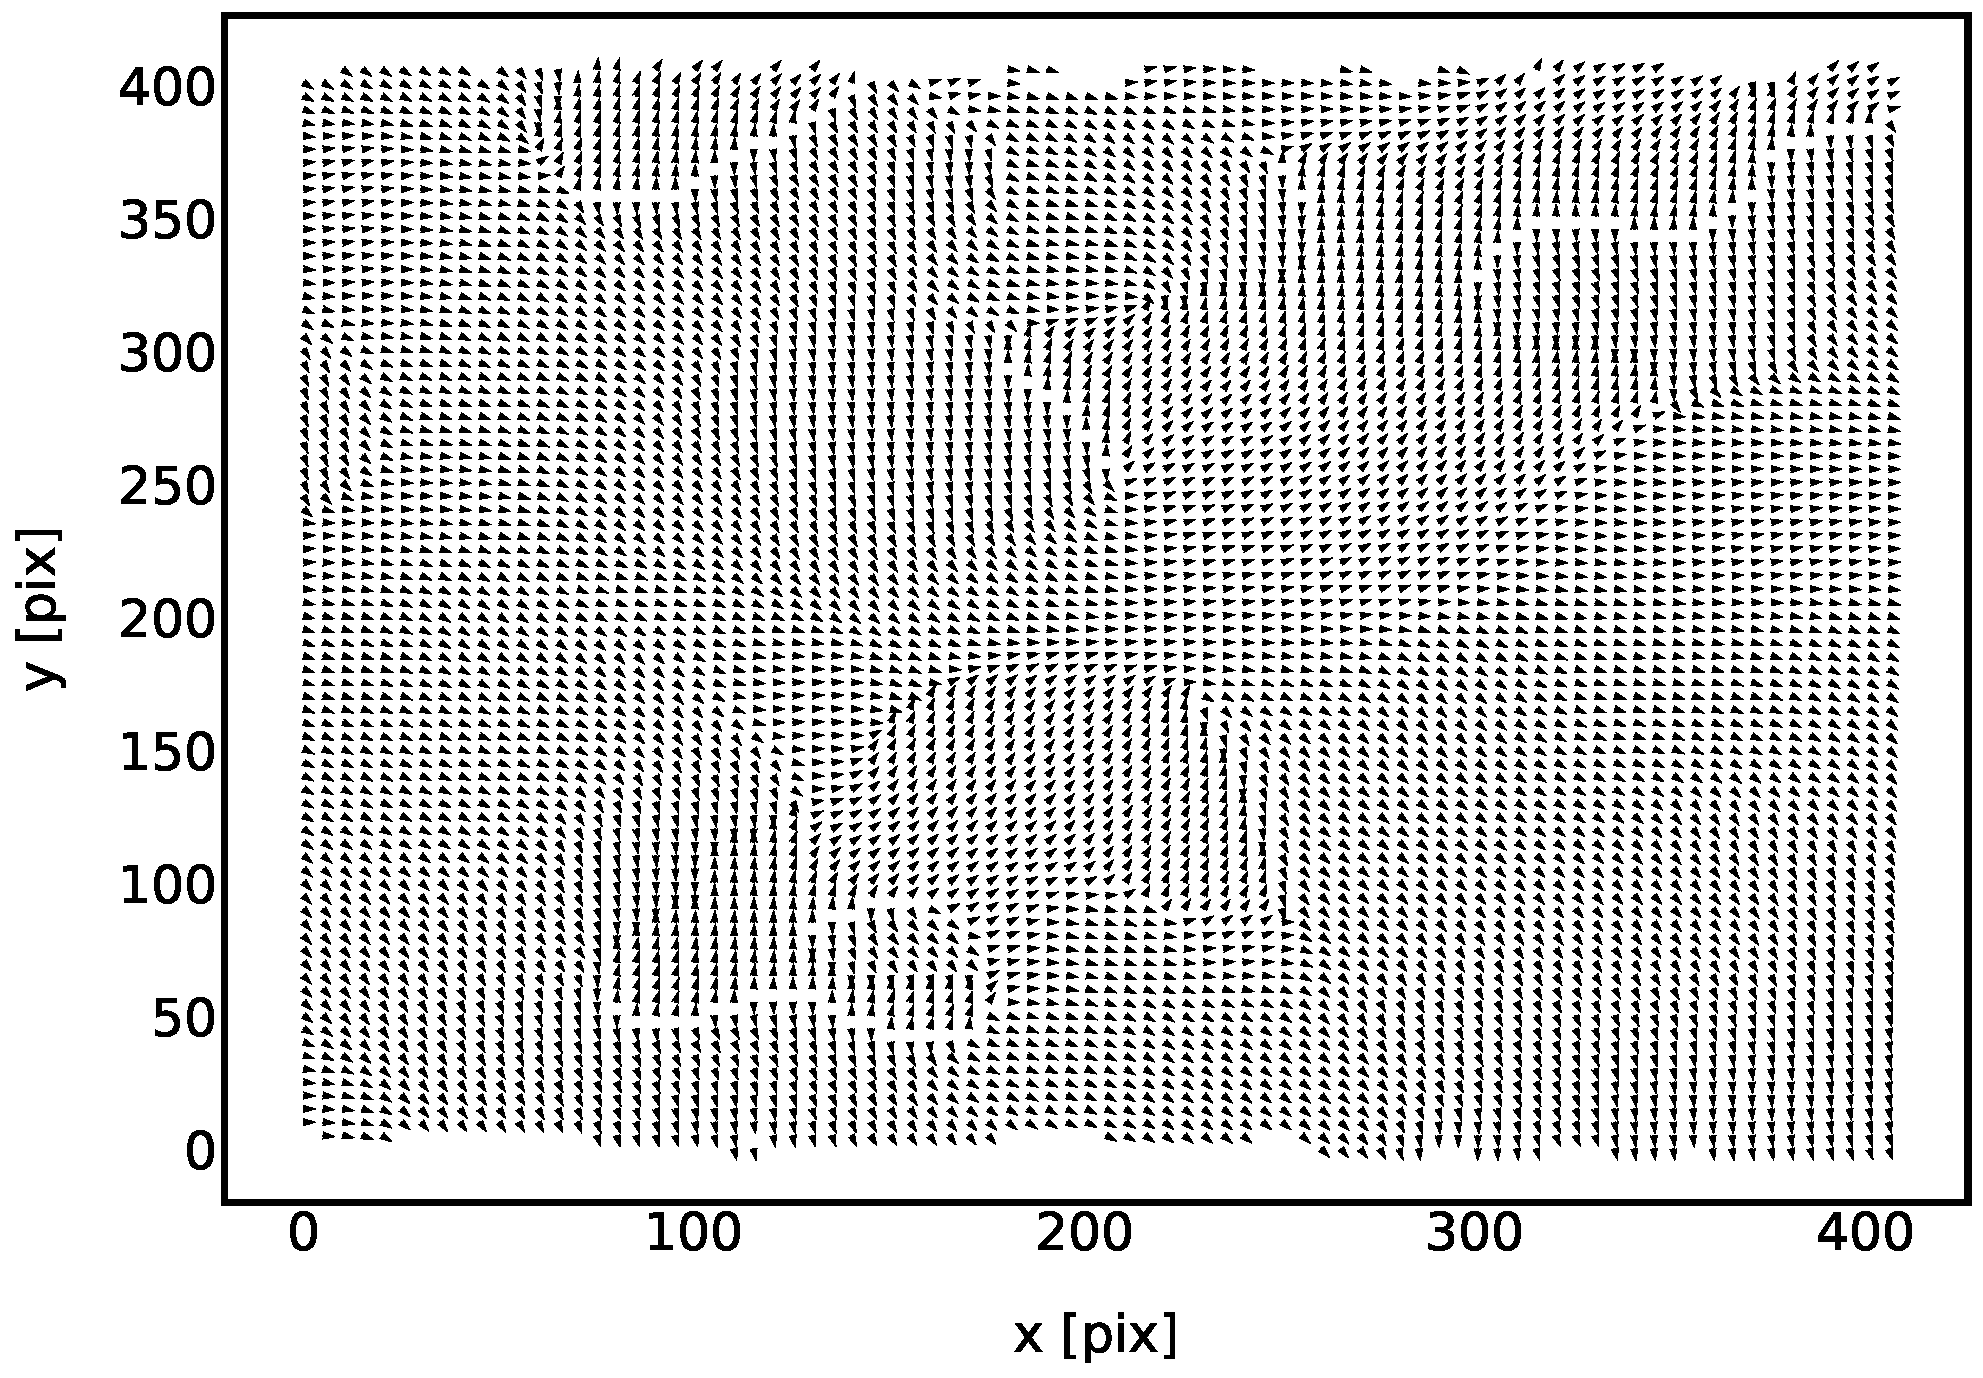
\includegraphics[width=\textwidth]{figures/carina/vectors_5}
\caption[The CNC polarization vector map, decimated by 5\macrocapwrap{$\times$}.]{The CNC polarization vector map, with \gls{vpol} following \gls{Bpos} and decimated by 5$\times$.}
\label{fig:vectors_5}
\end{figure}

\begin{figure}[!htbp]
\centering
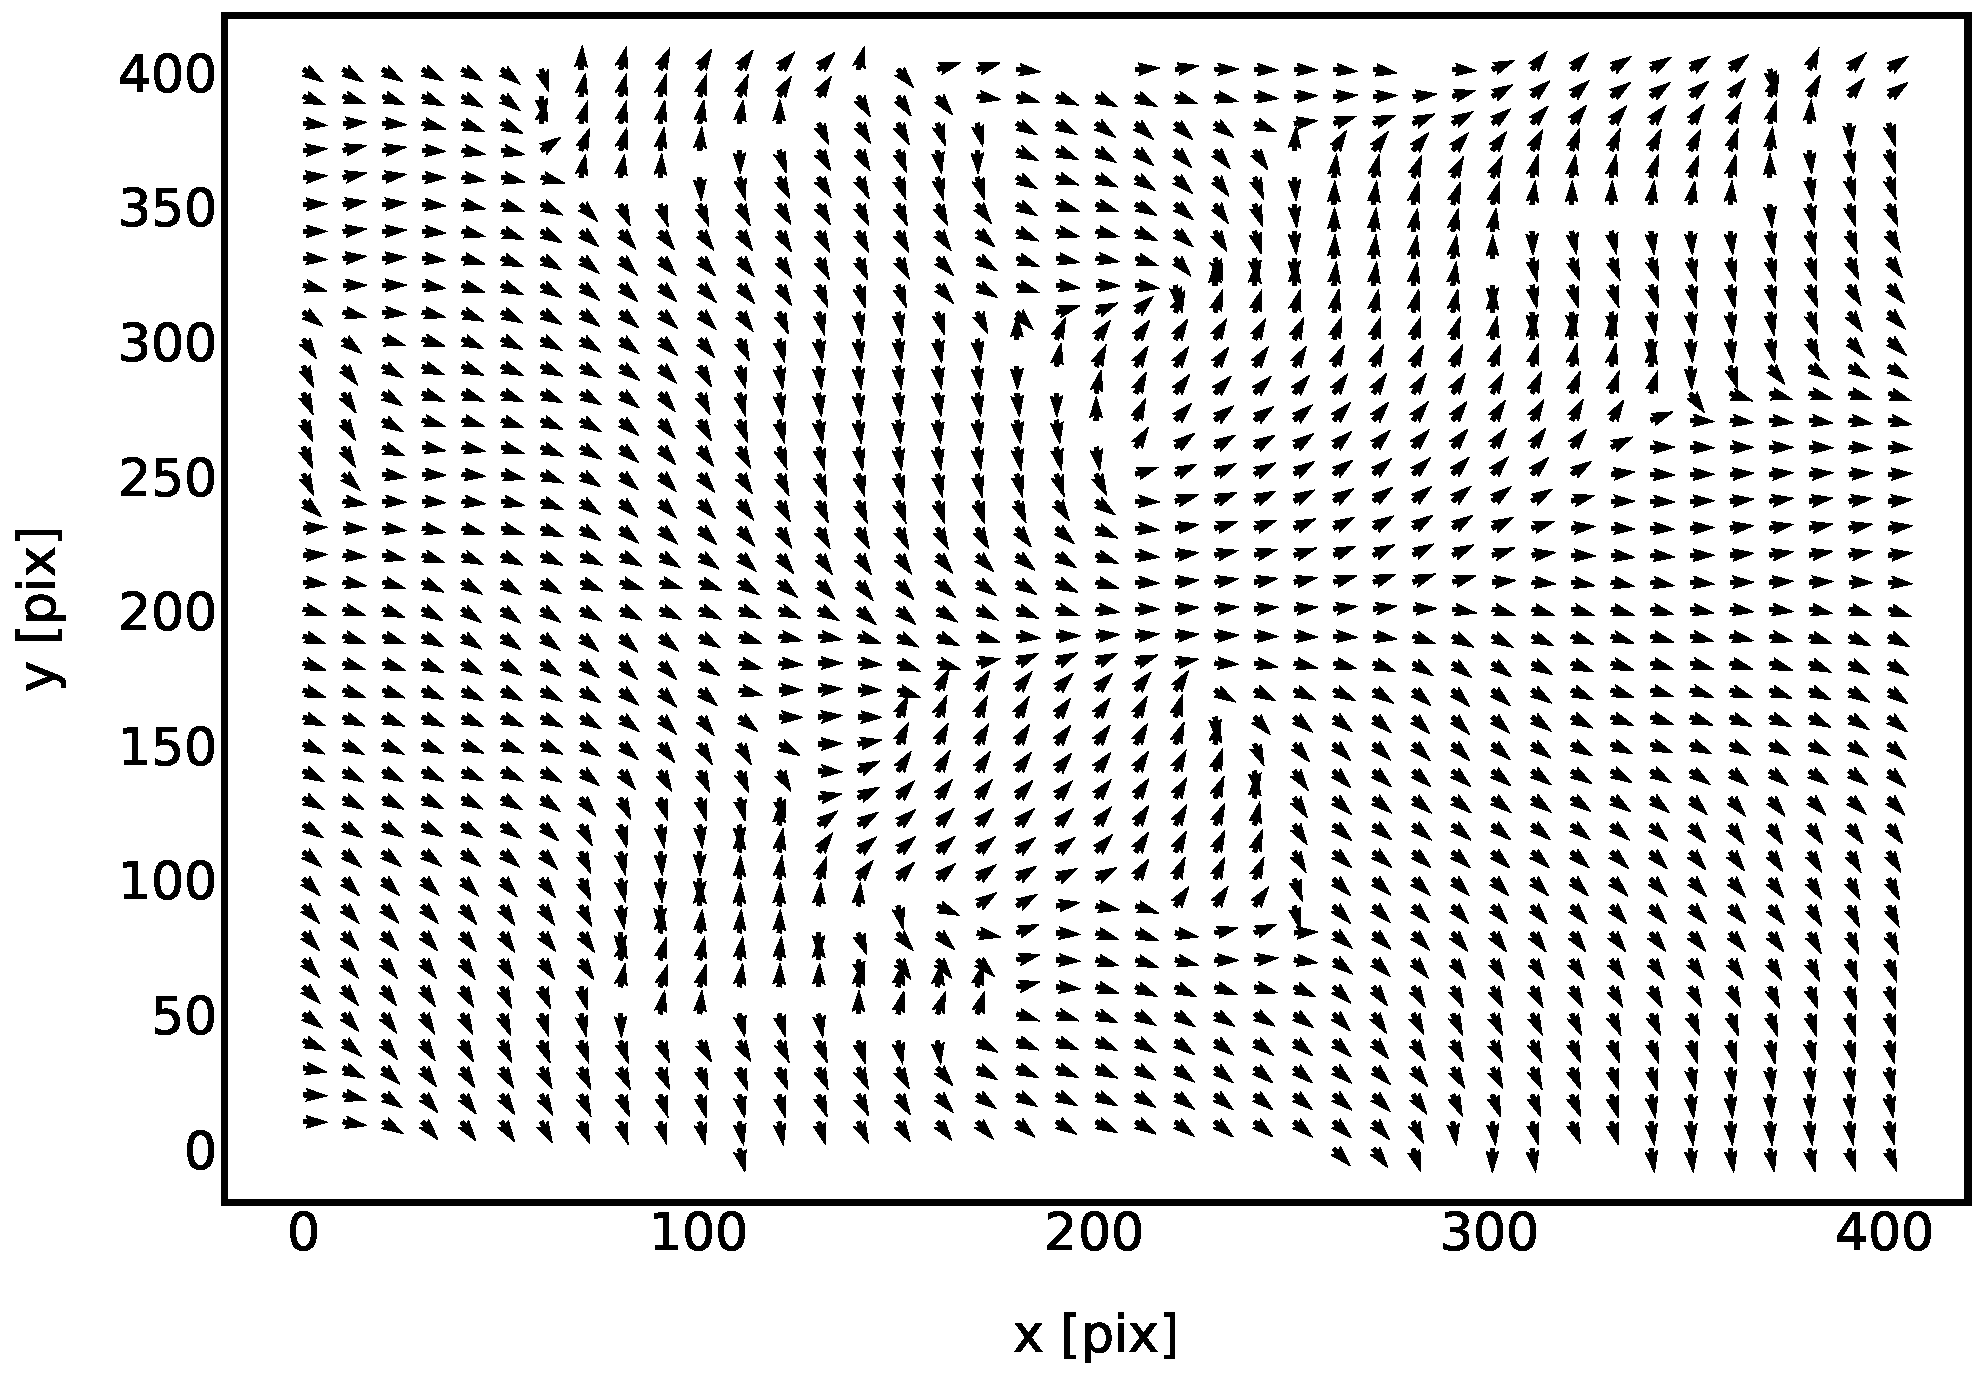
\includegraphics[width=\textwidth]{figures/carina/vectors_10}
\caption[The CNC polarization vector map, decimated by 10\macrocapwrap{$\times$}.]{The CNC polarization vector map, with \gls{vpol} following \gls{Bpos} and decimated by 10$\times$.}
\label{fig:vectors_10}
\end{figure}

\begin{figure}[!htbp]
\centering
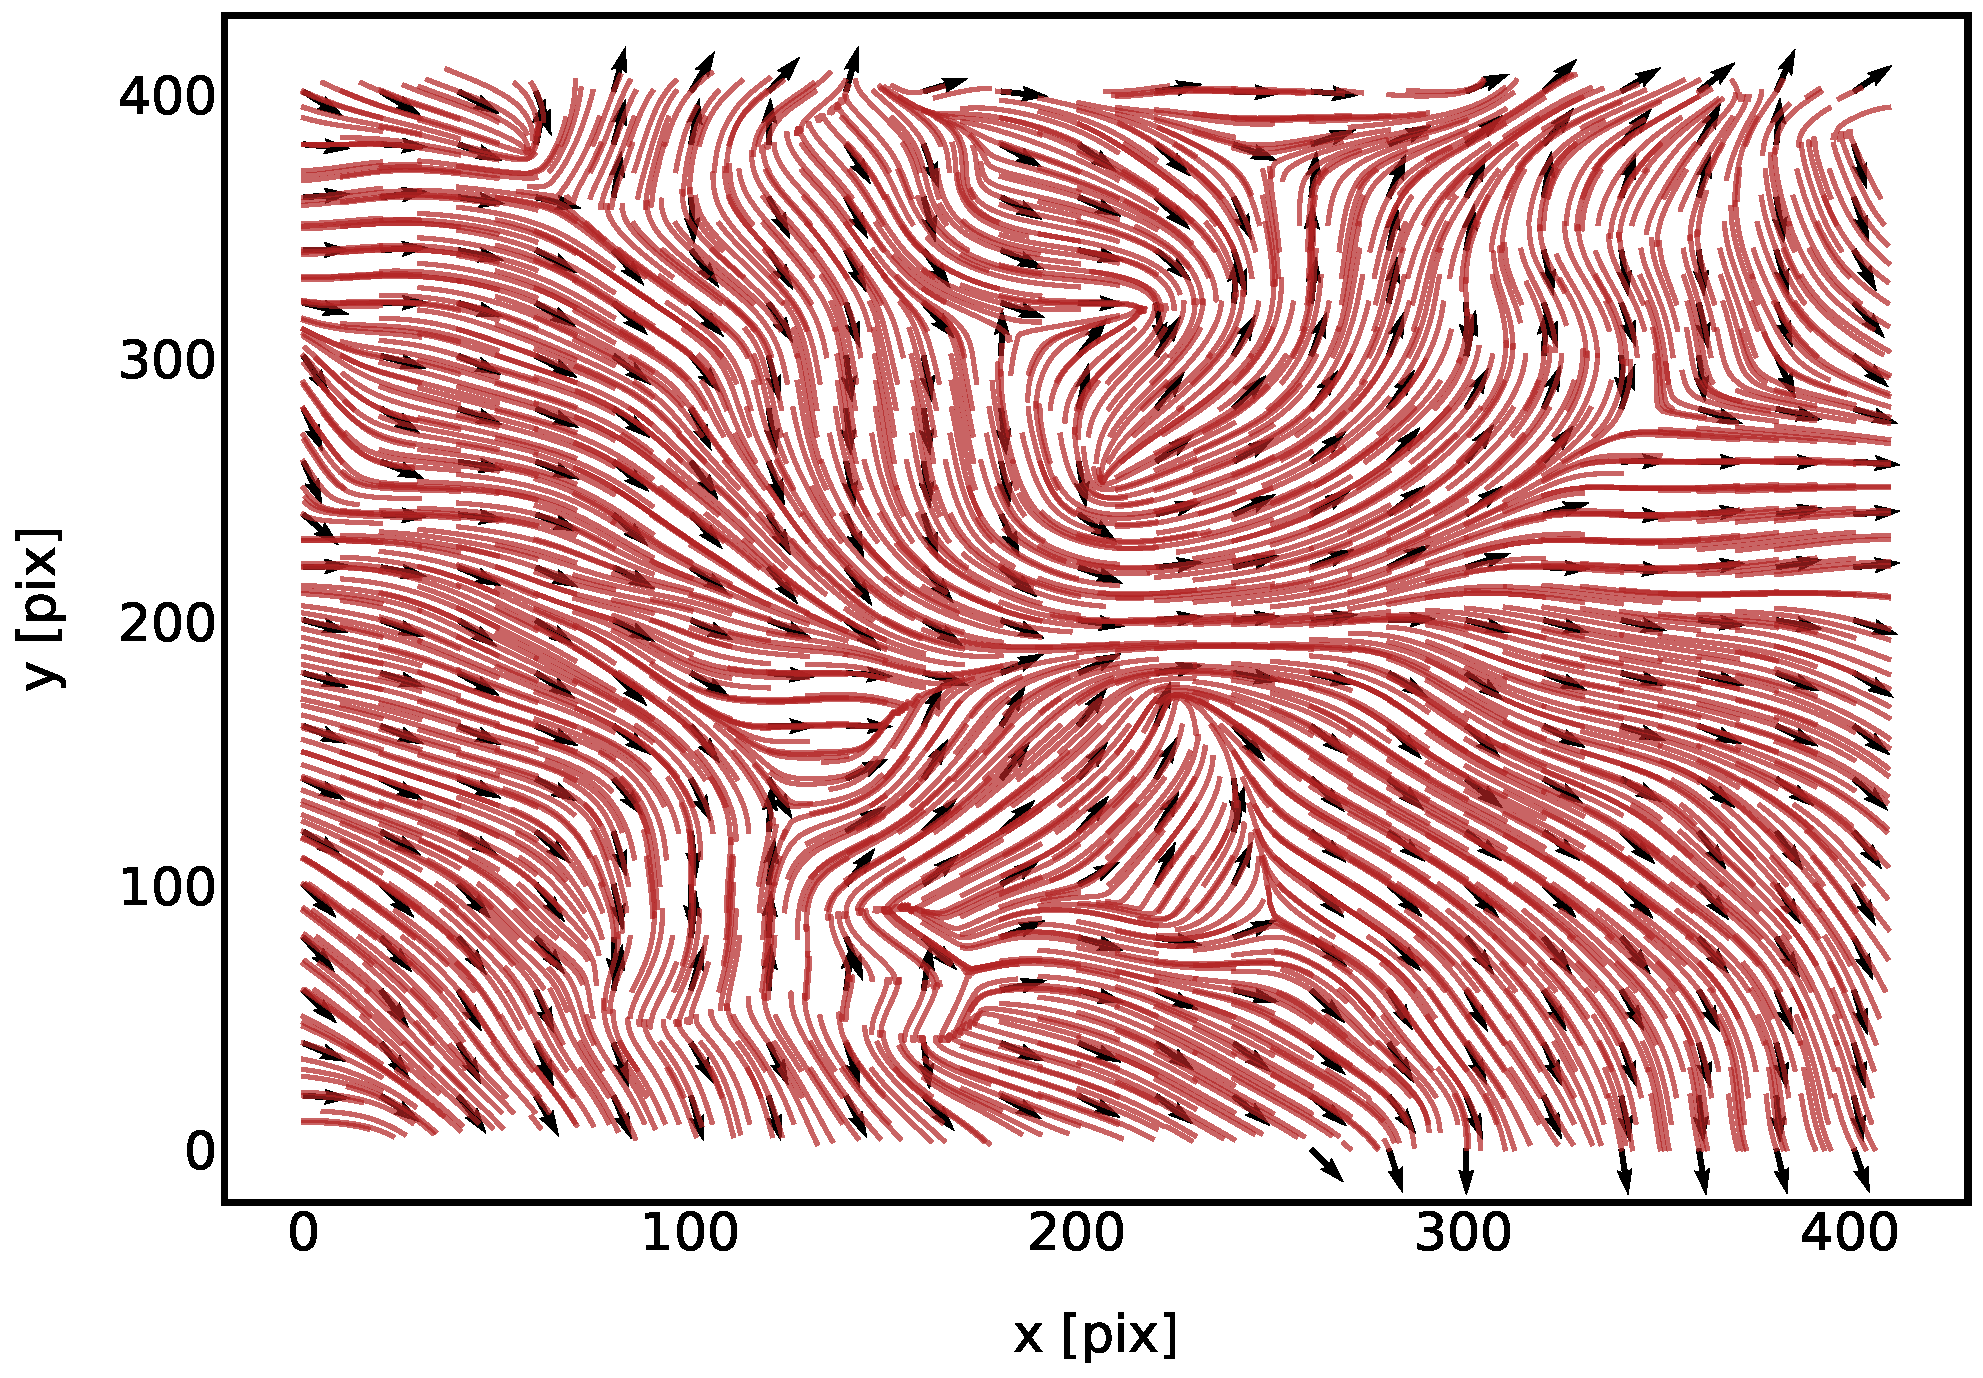
\includegraphics[width=\textwidth]{figures/carina/vector_sl_21_ds10}
\caption[The CNC polarization-streamline map, with streamlines decimated by 10\macrocapwrap{$\times$}.]{A CNC polarization streamline map, with the streamlines following \gls{Bpos} and decimated by 10$\times$.}
\label{fig:vector_sl_21_ds10}
\end{figure}

\begin{figure}[!htbp]
\centering
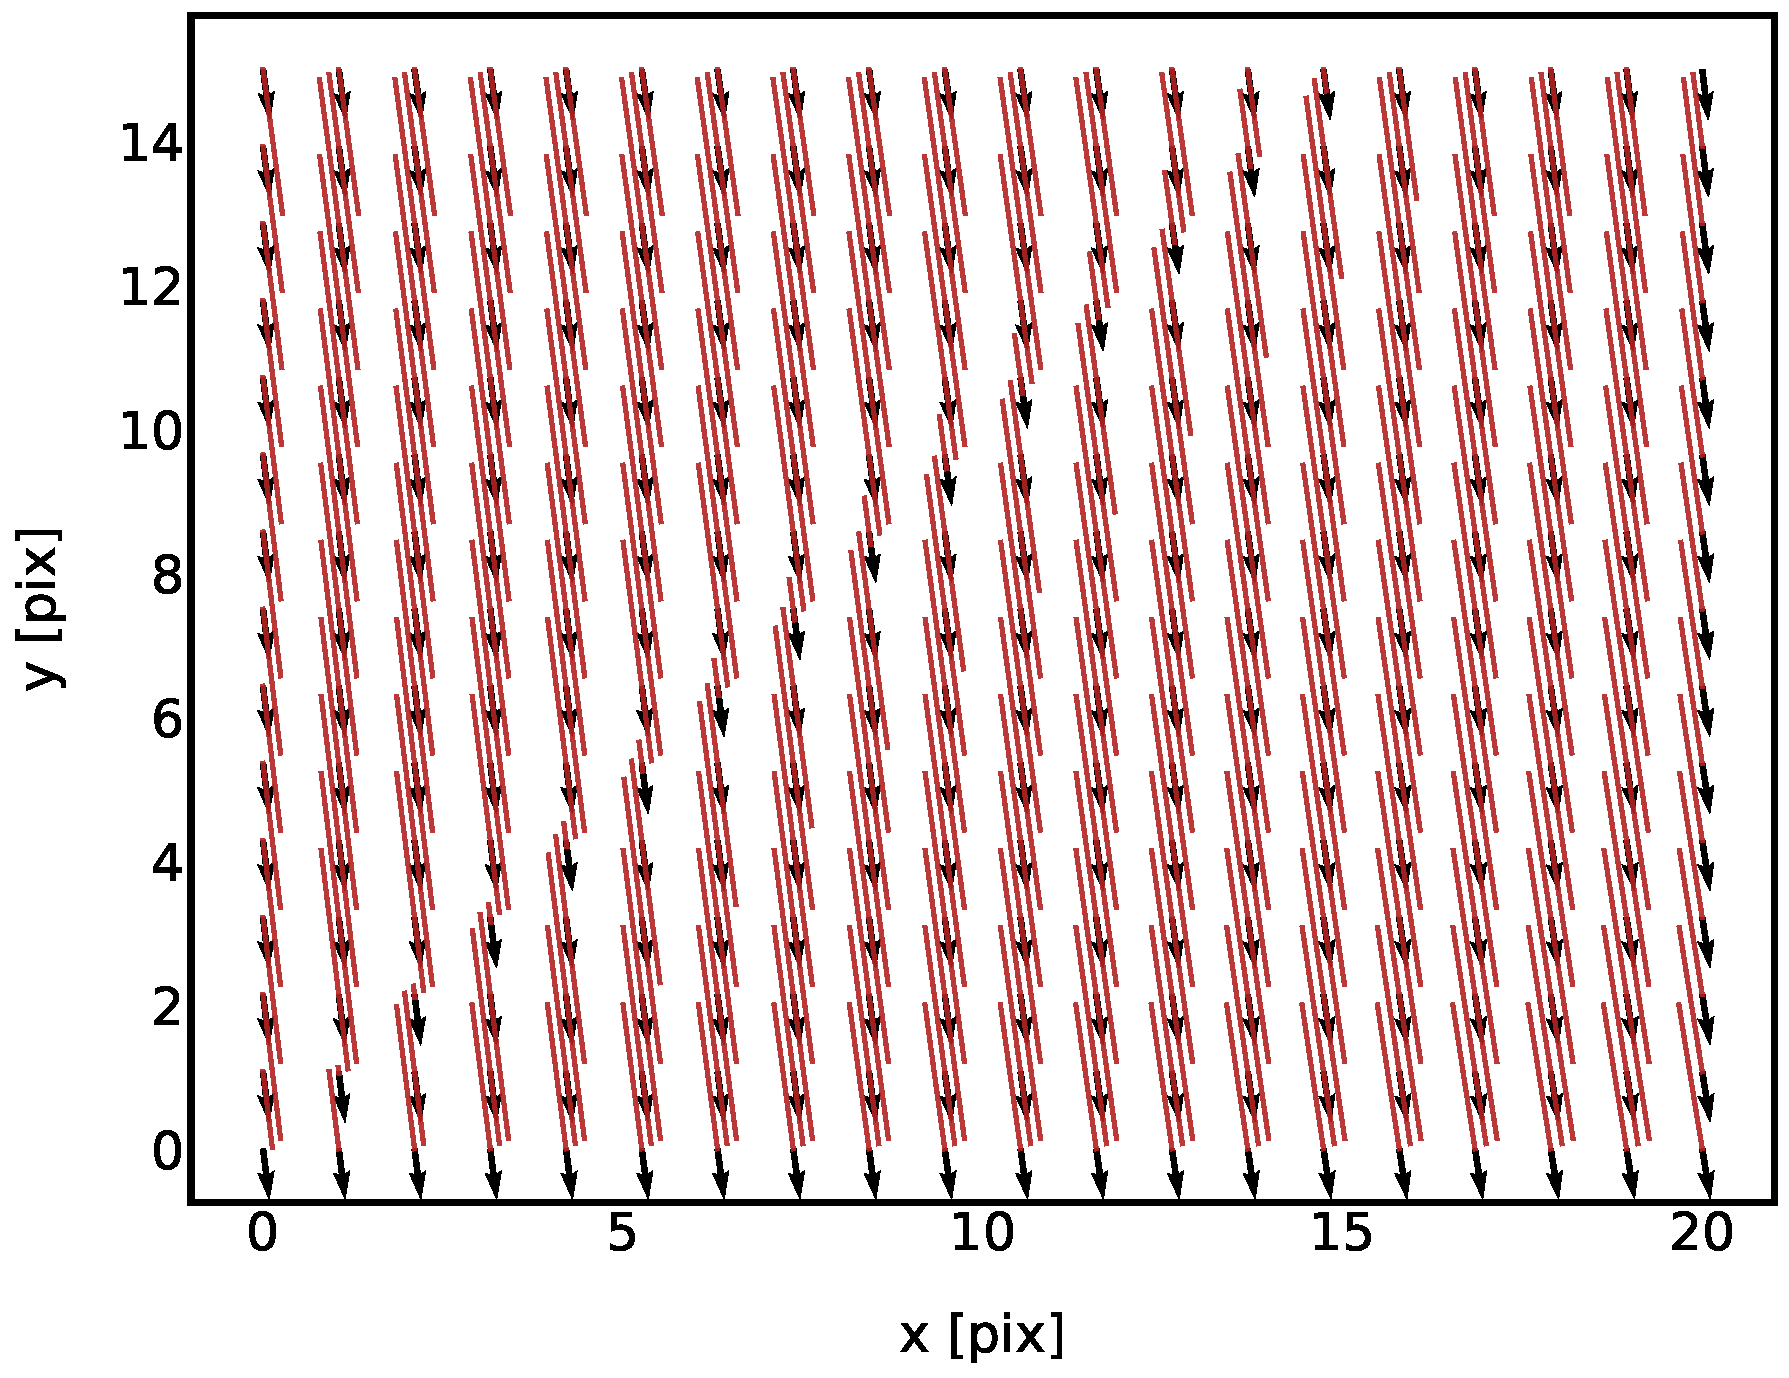
\includegraphics[width=\textwidth]{figures/carina/vector_sl_zoom}
\caption[A zoom-in of a uniform region of the vector-streamline map.]{A zoom-in of a region of the vector-streamline map where the polarization angles are very uniform.}
\label{fig:vector_sl_zoom}
\end{figure}

\begin{figure}[!htbp]
\centering
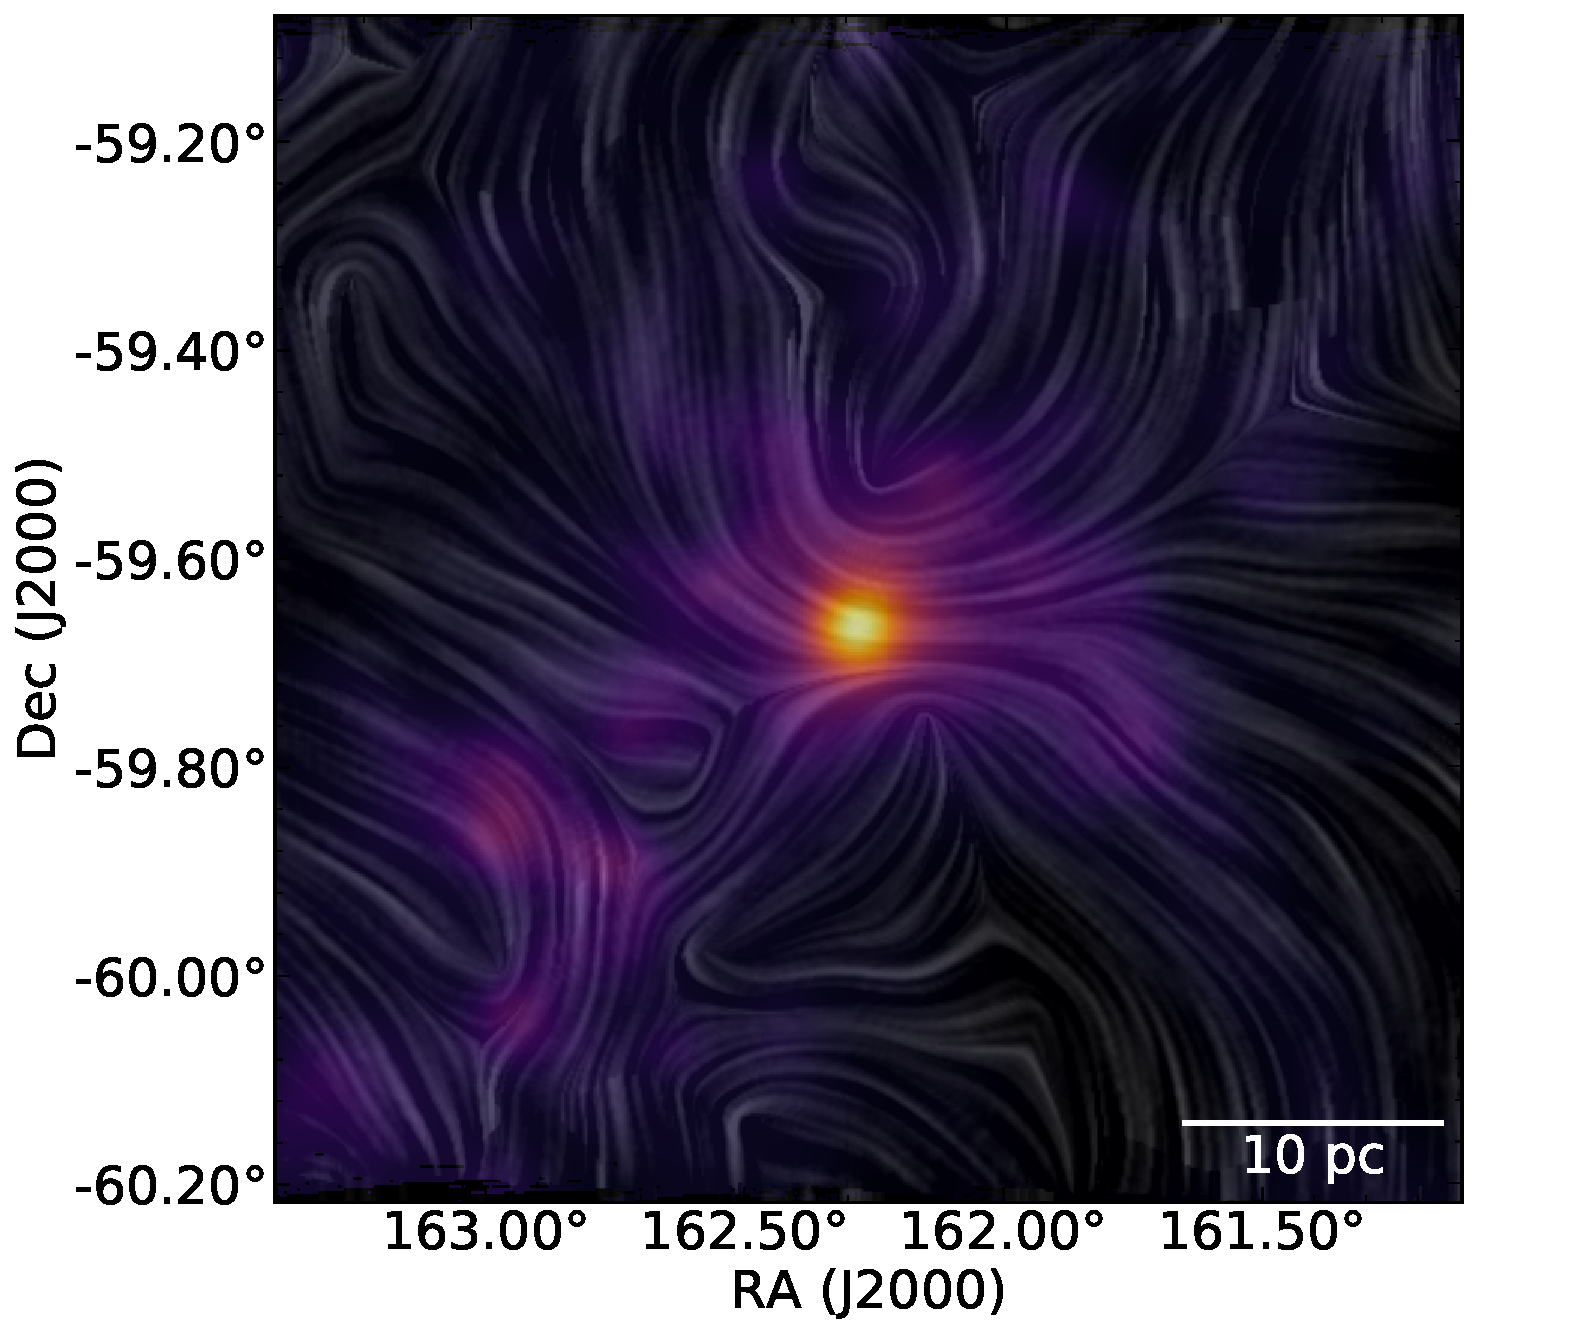
\includegraphics[width=\textwidth]{figures/carina/lic_han_51}
\caption[The \macrocapwrap{LIC$_{500}$} map, displayed as a transparent overlay on the \macrocapwrap{$I_{500}$} map.]{The LIC$_{500}$ map, displayed as a transparent overlay on the $I_{500}$ map.}
\label{fig:lic_han_51}
\end{figure}

\begin{figure}[!htbp]
\centering
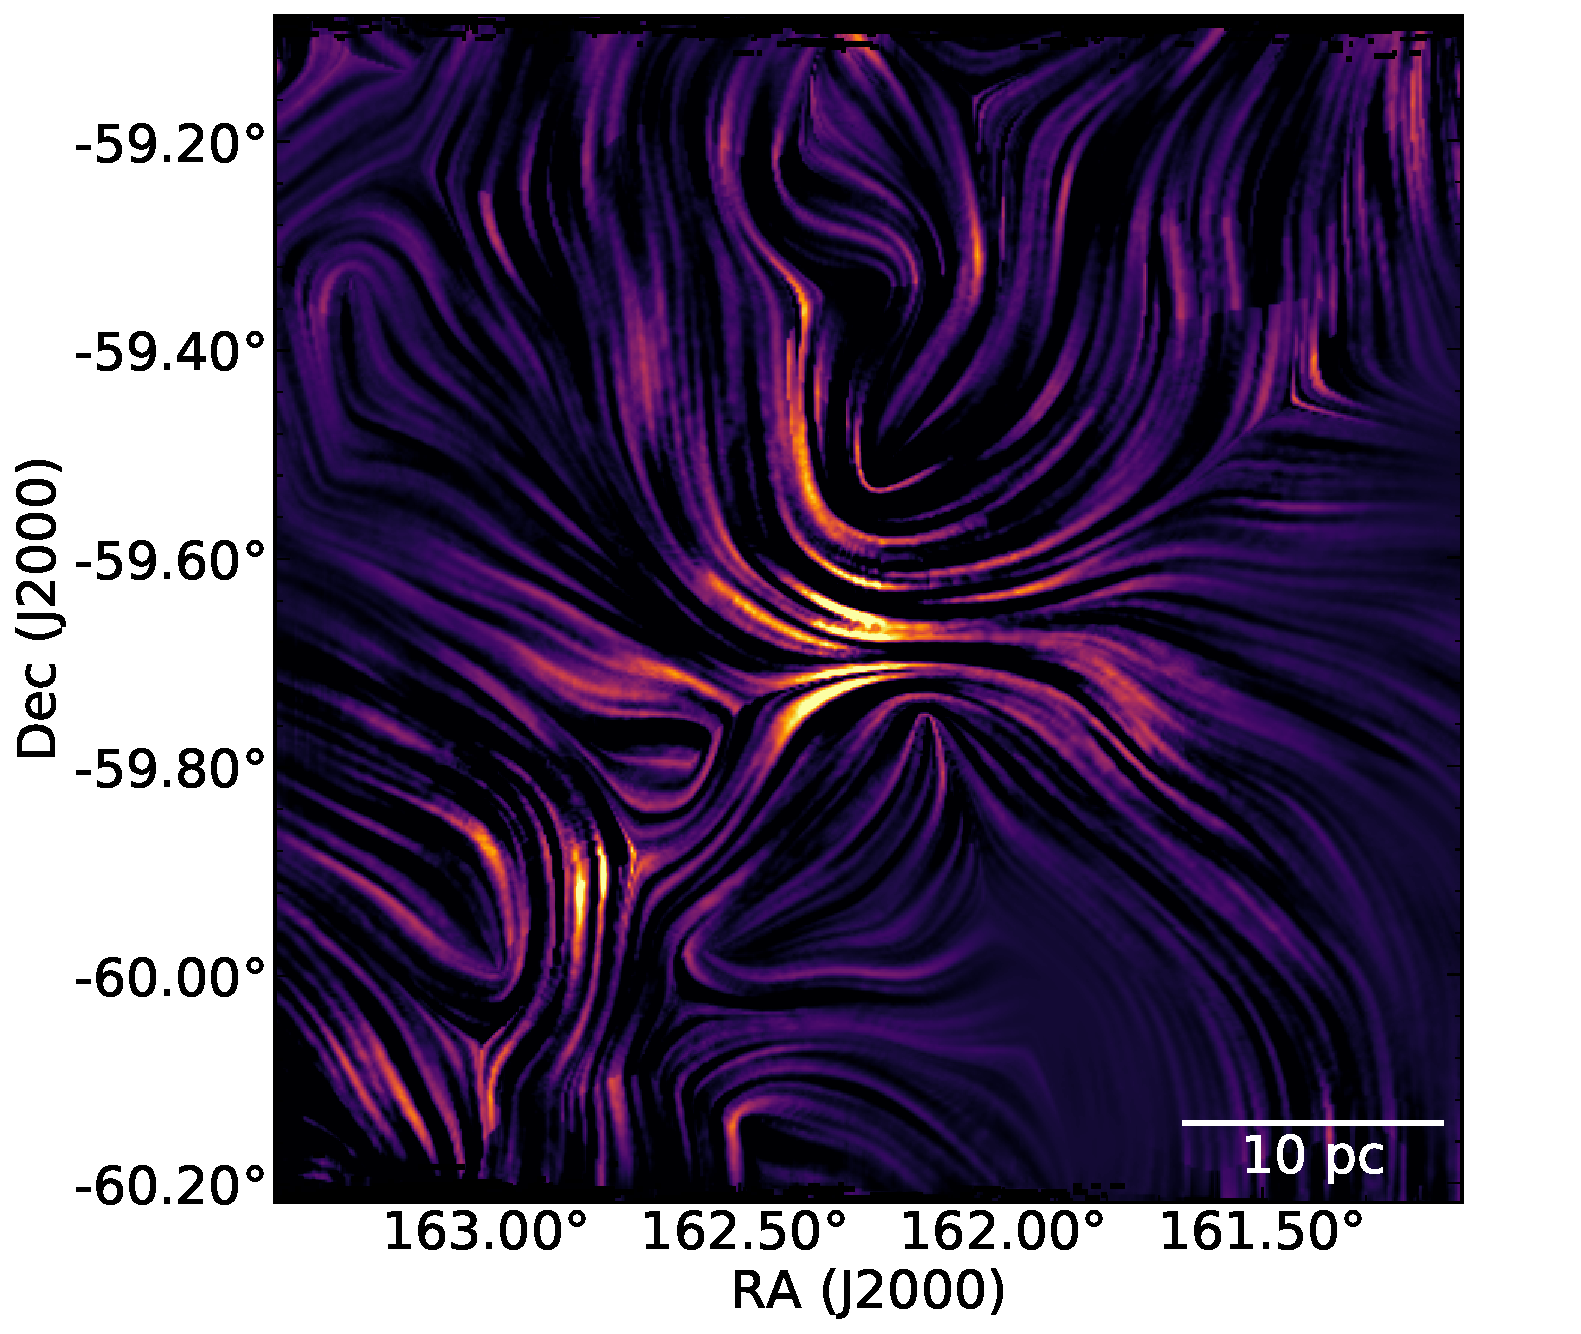
\includegraphics[width=\textwidth]{figures/carina/lic2_han51}
\caption[An intensity-weighted \macrocapwrap{LIC$_{500}$} map, displayed with an aggressive intensity stretch.]{An intensity-weighted LIC$_{500}$ map, displayed with an aggressive intensity stretch.}
\label{fig:lic2_han51}
\end{figure}

\begin{figure}[!htbp]
\centering
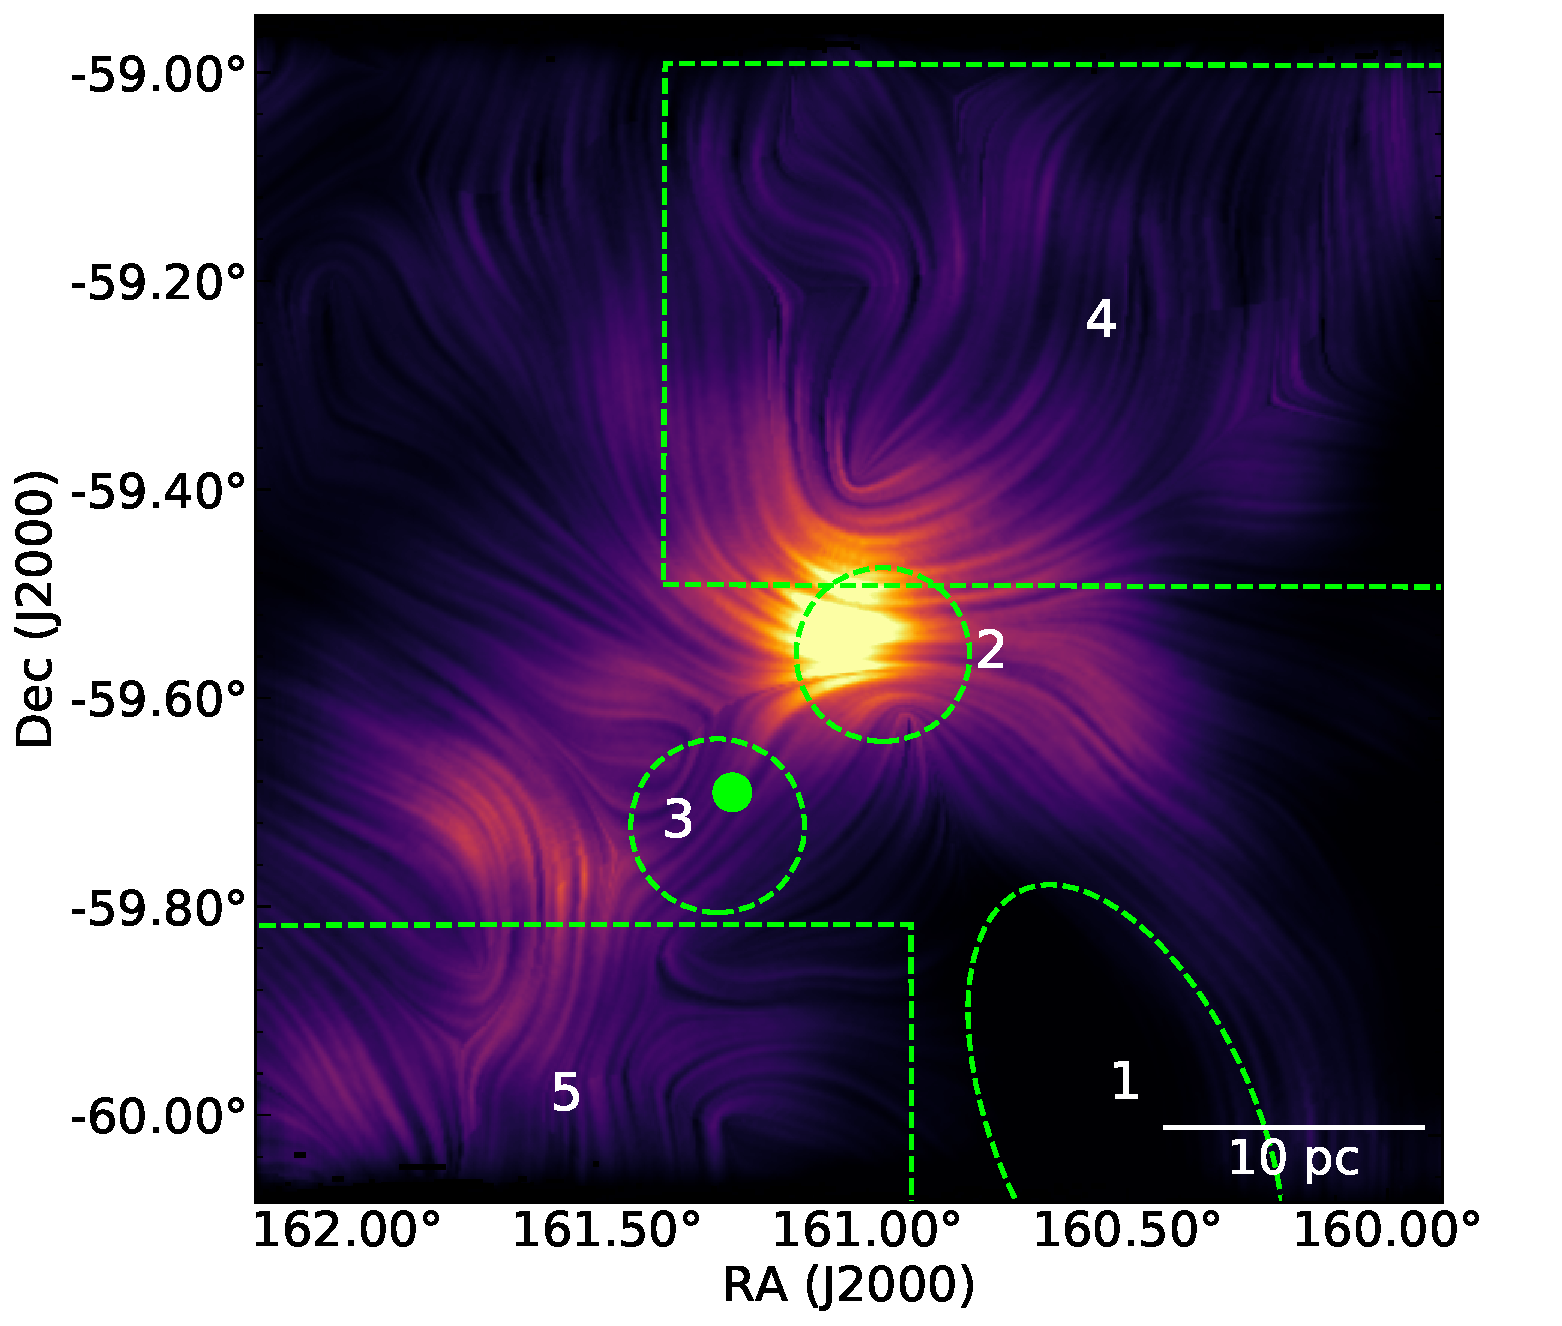
\includegraphics[width=\textwidth]{figures/carina/lic_mult}
\caption[A less aggressive stretch of the intensity-weighted \macrocapwrap{LIC$_{500}$}.]{A less aggressive stretch of the intensity-weighted LIC$_{500}$. The numbered regions are listed in Table~\ref{table:regions}, and discussed in Section~\ref{multiband comp}}.
\label{fig:lic_map}
\end{figure}

\section{Multiwavelength Observations of the CNC}\label{multiband comp}

The CNC (10h 45m 08.5s -59$^{\circ}$ 52$\arcmin$ 04$\arcsec$) is a bright Galactic giant molecular cloud (GMC) which is host to several HII regions and active massive star formation. Its distance is estimated at $\sim$2.3~kpc (\citet{allen1993shape,smith2006structure}). However, recent observations by the Gaia space observatory have found that the distance might be closer to 2.6~kpc \citep{davidson2018gaia}. In this analysis, we assume the more commonly used distance of 2.3~kpc. Although the CNC occupies an area of $\sim$5~deg$^{2}$, in this work we focus on the inner $\sim$1.25~deg$^{2}$.

First discovered in 1752, the CNC has been well studied across the electromagnetic spectrum (see e.g., \citet{smith2008carina}). It is estimated to contain $\sim$25,000 M$_{\odot}$ of material, which includes part of the Carina OB1 association. The inner region of the CNC contains the Homunculus and Keyhole nebulas, as well as two massive open clusters, Trumpler 16 (Tr~16) and Trumpler 14 (Tr~14). Tr~16, the more evolved of the two clusters, is host to two of the brightest star systems in the Milky Way: $\eta$ Car, a binary system which is known for its strong wind-wind interactions, and WR 25. Tr~14 is thought to be just 0.5~Myr old \citep{preibisch2011hawk}.

Ionizing stellar winds which are driven by large OB associations have carved out several conspicuous bubbles throughout the CNC\@. The most prominent of these is the GUM 31 nebula, to the northwest of Tr~16. Smaller groups of bubbles are visible to the north and south of Tr~16. The variety of high energy processes occurring within the CNC make it an ideal laboratory for the study of stellar feedback and triggered star formation.

The CNC has been observed in the sub-mm/FIR/mm-wave by ground-based (LABOCA, \citep{preibisch2011laboca}, SPARO \citep{li2006results}), balloon-borne (BLASTPol, \citep{shariff2019submillimeter} and space-based telescopes (e.g., Planck, \citep{abergel2014planck}, Herschel, (\citet{preibisch2012herschel,gaczkowski2013herschel,roccatagliata2013herschel})). Spectral data in the submillimeter has also been obtained \citep{oberst2006detection}. The authors of \citet{li2006results} presented the first maps of \gls{Bpos} pseudovectors in the inner region of the CNC\@. In their analysis of $\sim$30 pseudovectors within the inner 1~deg$^{2}$ of the CNC, they found that the mean position angle of \gls{Bpos} is within $\approx$ 15~deg of the GP\@. They also observed that the pseudovectors to the north and south of the central region appear to run parallel to a section of the perimeters of two large HII regions. Figure~\ref{fig:lic_sparo_overlay} illustrates the overlap between the SPARO and BLASTPol map coverages.

% SPARO overlay
\begin{figure}[!htbp]
\centering
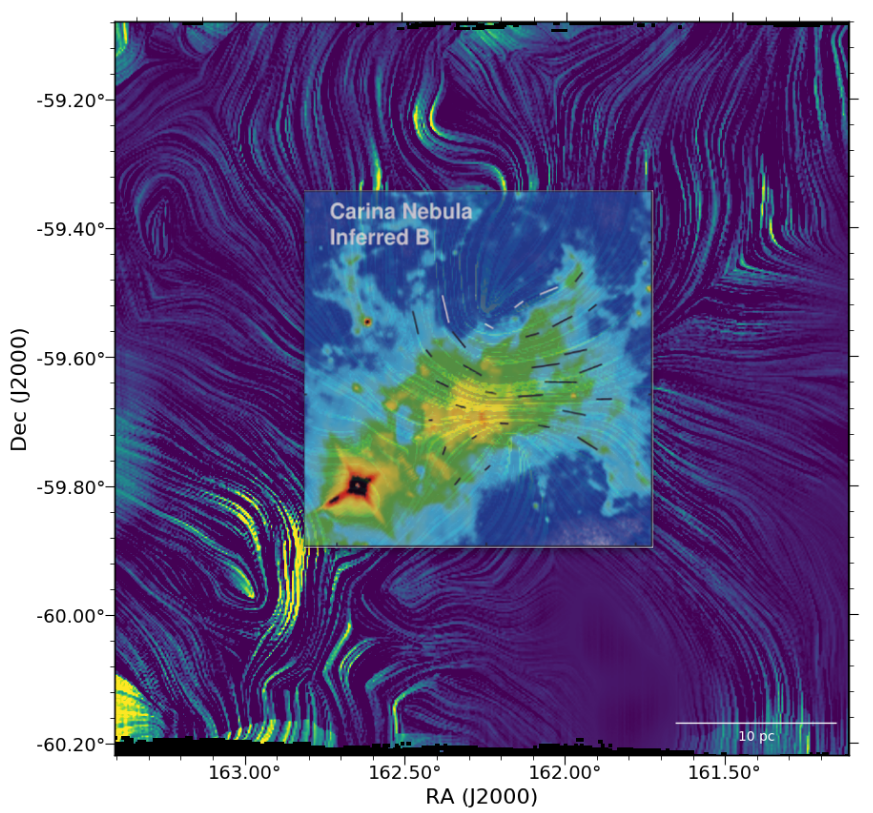
\includegraphics[width=\textwidth]{figures/carina/lic_sparo_overlay}
\caption[The CNC intensity map taken by SPARO overlayed on the \macrocapwrap{$\sim$1.25~deg$^{2}$} of the BLASTPol CNC map.]{The CNC intensity map taken by SPARO \citep{li2006results}, with polarization vectors (inset), overlayed on the $\sim$1.25~deg$^{2}$ of the BLASTPol CNC map.}
\label{fig:lic_sparo_overlay}
\end{figure}

Besides BLASTPol and SPARO, the multi-band Planck data constitutes the only polarized sub-mm observations of the CNC to date. In this work, only the Planck 353~GHz (850~$\upmu$m) maps are used as part of the quantitative analysis.

The Herschel maps constitute the highest resolution FIR maps of the CNC, revealing physical structures in the dust on spatial scales of 0.1--0.4~pc. This spatial scale is thought to correspond to the upper size limit of the filamentary structures which thread the CNC, and which are observed in other MCs. In this analysis, the smoothed resolution of 5$\arcmin$ corresponds to a physical scale of $\sim$3.5~pc, which is well above the scale of individual filaments. However, this physical resolution is sufficient to gain insight into the larger scale structures seen in the CNC\@.

% Regions table
\begin{table}[!htbp]
\centering
\begin{tabular}{@{}ll@{}}
\dtoprule{}
Region \# & Name \\ \midrule
1 & Southern Bubble (SB) \\
2 & Tr~14 \\
3 & Tr~16 \\
4 & Northern Bubbles (NB) \\
5 & Southern Pillars (SP) \\ \dbottomrule{}
\\
\end{tabular}
\caption[Regions of interest inside the inner \macrocapwrap{$\sim$1.25~deg$^{2}$} of the BLASTPol CNC map.]{Regions of interest inside the inner $\sim$1.25~deg$^{2}$ of the BLASTPol CNC map. These regions correspond to those used in \citet{preibisch2012herschel}.}
\label{table:regions}
\end{table}

The most visible structures revealed in the Herschel maps are discussed in detail in \citet{preibisch2012herschel}. The main features which occur in the inner $\sim$1~deg$^{2}$ of the CNC (and which are visible in the BLASTPol maps) are briefly described below. These features are listed in Table~\ref{table:regions}. Figures~\ref{fig:msx_overplot} through~\ref{fig:chandra_overplot} show semi-transparent overlays of the BLASTPol $I_{250}$ dust maps (in red) with maps in the near-infrared (NIR) (8~$\upmu$m, Midcourse Space Experiment (MSX, \citet{smith2000large}), R-band (Guide Star Catalog II (GSC2), Palomar and UK Schmidt telescopes \citep{lasker2008second}) and soft X-ray (Chandra Carina Complex Project \citep{townsley2011introduction}). The B-field streamlines produced using Eulerian advection (see Section~\ref{LIC}) are overplotted in yellow.

The most prominent features in the sub-mm/FIR maps of the CNC are the voids, or bubbles, to the north and south of Tr~14 and Tr~16. Following \citet{preibisch2012herschel}, we denote these as the Northern Bubbles (NB) and the Southern Bubble (SB). The SB appears as an elongated void to the southwest of Tr~16, with its long axis spanning $\sim$30~pc. Although the southern extent of the bubble is not visible in the BLASTPol map, a clear, rounded boundary can be seen in the Herschel map. The authors of \citet{preibisch2012herschel} identify three early-type stars which are potentially located inside the bubble. They point out that the three stars alone most likely do not constitute an energy source which is sufficient enough to have created the SB by way of stellar winds and ionizing radiation. They offer two possible explanations for its origin: 1) That the bubble could be the result of gas which has been forced out of the central part of the CNC, and 2) that the bubble might be the lower lobe of a bipolar jet formed by stars in the Tr~16 cluster.

The multiband overlay maps support the hypothesis that the Southern Bubble is an enclosed, three-dimensional void. Its edges are well defined by ionized gas which is visible in the R-band map. The Chandra map reveals that the bubble is in fact filled with hot, diffuse gas (T $\geq$ 10$^{4}$~K). At 8~$\upmu$m, the emission is from polycyclic aromatic hydrocarbons (PAHs) which have been vibrationally energized by the absorption of far-UV photons. As discussed in \citet{li2006results}, the intensity of the 3--11~$\upmu$m PAH spectrum depends on the ratio of the intensity of the far-UV radiation field to the electron density. Whereas the electron density changes abruptly across the edges of HII regions, the intensity of the illuminating radiation field does not. Therefore, PAH emission is an excellent tracer of the boundaries of HII regions. This effect is visible in the 8~$\upmu$m overlay, shown in Figure~\ref{fig:msx_overplot}.

The direction of the \gls{Bpos} streamlines shown in the overlay images appear to be well correlated with the edges of the SB\@. Along the boundaries of the SB, \gls{Bpos} is largely parallel to the bubble edges (particularly along the western boundary), which is the expected behavior under the conditions of B-field flux-freezing \citep{li2006results} (see below).

Unlike the SB, the NB does not appear to be a single HII region. The Herschel maps show it to be a combination of several smaller HII regions which have merged, forming dust clouds and pillars at their intersections. In the multi-band images, then boundaries of individual voids within the NB region are less defined than those of the SB, with the Chandra map showing a more diffuse concentration of ionized gas. However, as with the SB, the \gls{Bpos} streamlines in the NB region do appear to trace out the shape of a large, semi-spherical bubble. This is especially true for the southern boundary of the NB\@.

The brightest region of the BLASTPol maps is the central region of the CNC, located between Tr~16 and Tr~14. The eastern edge of Tr~14 is a well-studied photon dominated region (PDR) (see, e.g., \citet{kramer2008clumpy}). The edge of the PDR is loosely defined by the \gls{Bpos} streamlines. The region around Tr~16 is also well defined, with the streamlines appearing to trace out a bubble. The bubble's diameter is $\sim$3~pc, which is small in comparison to the SB and NB, with a diameter of $\sim$3~pc. Below this bubble is the region which \citet{preibisch2012herschel} denotes as the Southern Pillars (SP). This region of pillars is a site of active star formation, and has been shown to contain many compact IR sources \citep{smith2010spitzer}.

\begin{figure}[!htbp]
\centering
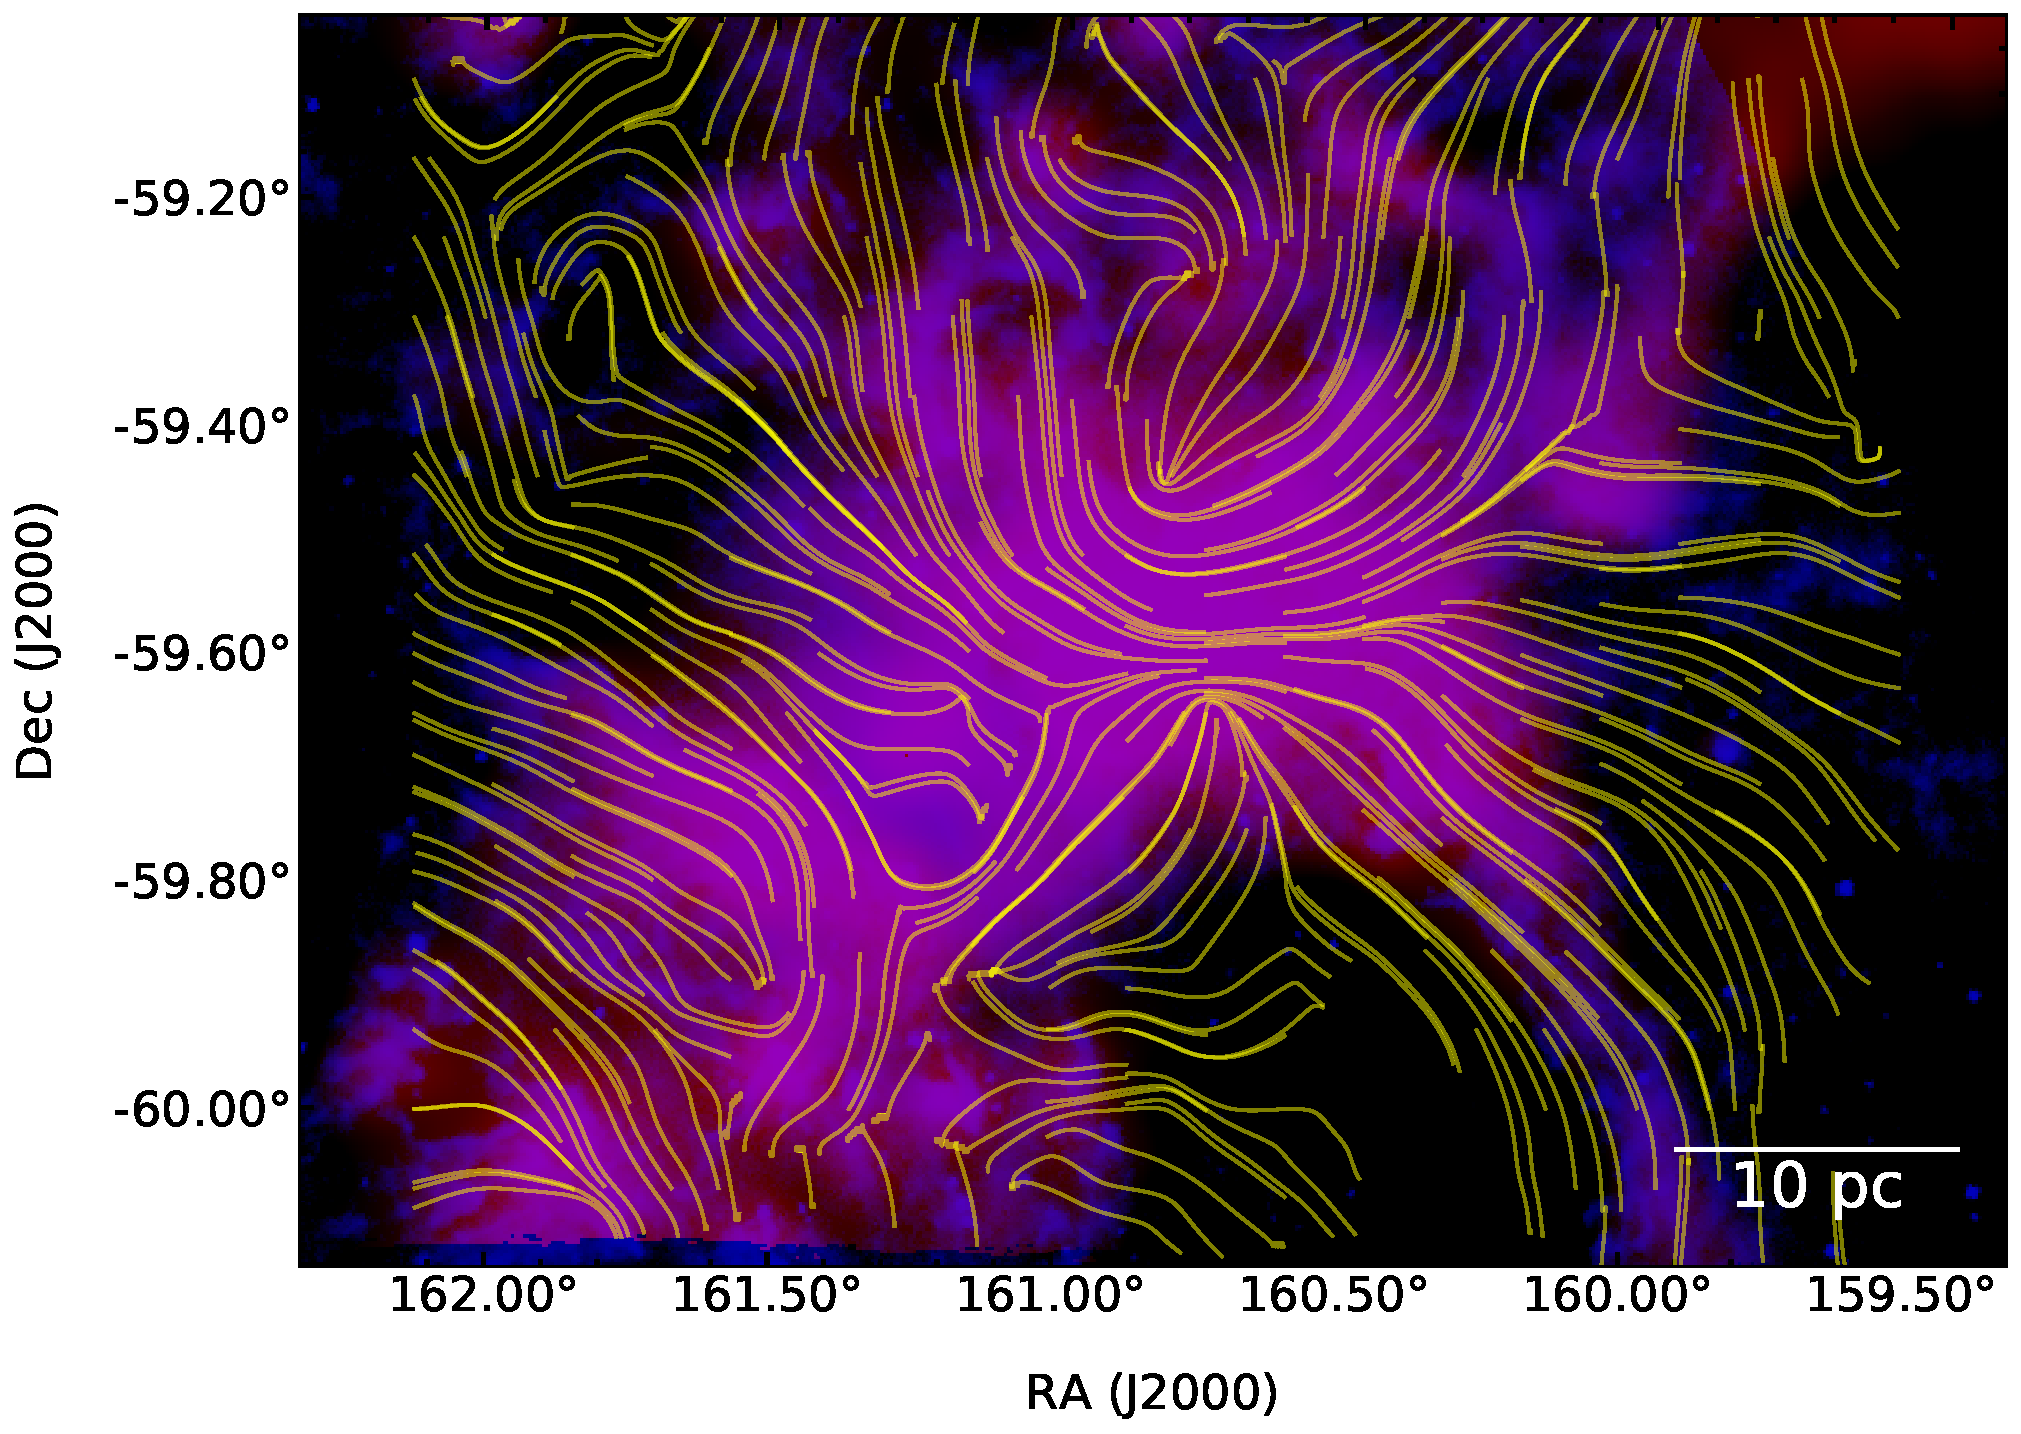
\includegraphics[width=\textwidth]{figures/carina/msx2_sl}
\caption[An overlay of the MSX \macrocapwrap{8~$\upmu$m} CNC map (green) with a BLASTPol intensity map (red).]{An overlay of the MSX 8~$\upmu$m CNC map (green) \citep{smith2000large} with a BLASTPol intensity map (red). A subset of polarization vector streamlines are overplotted in yellow.}
\label{fig:msx_overplot}
\end{figure}

\begin{figure}[!htbp]
\centering
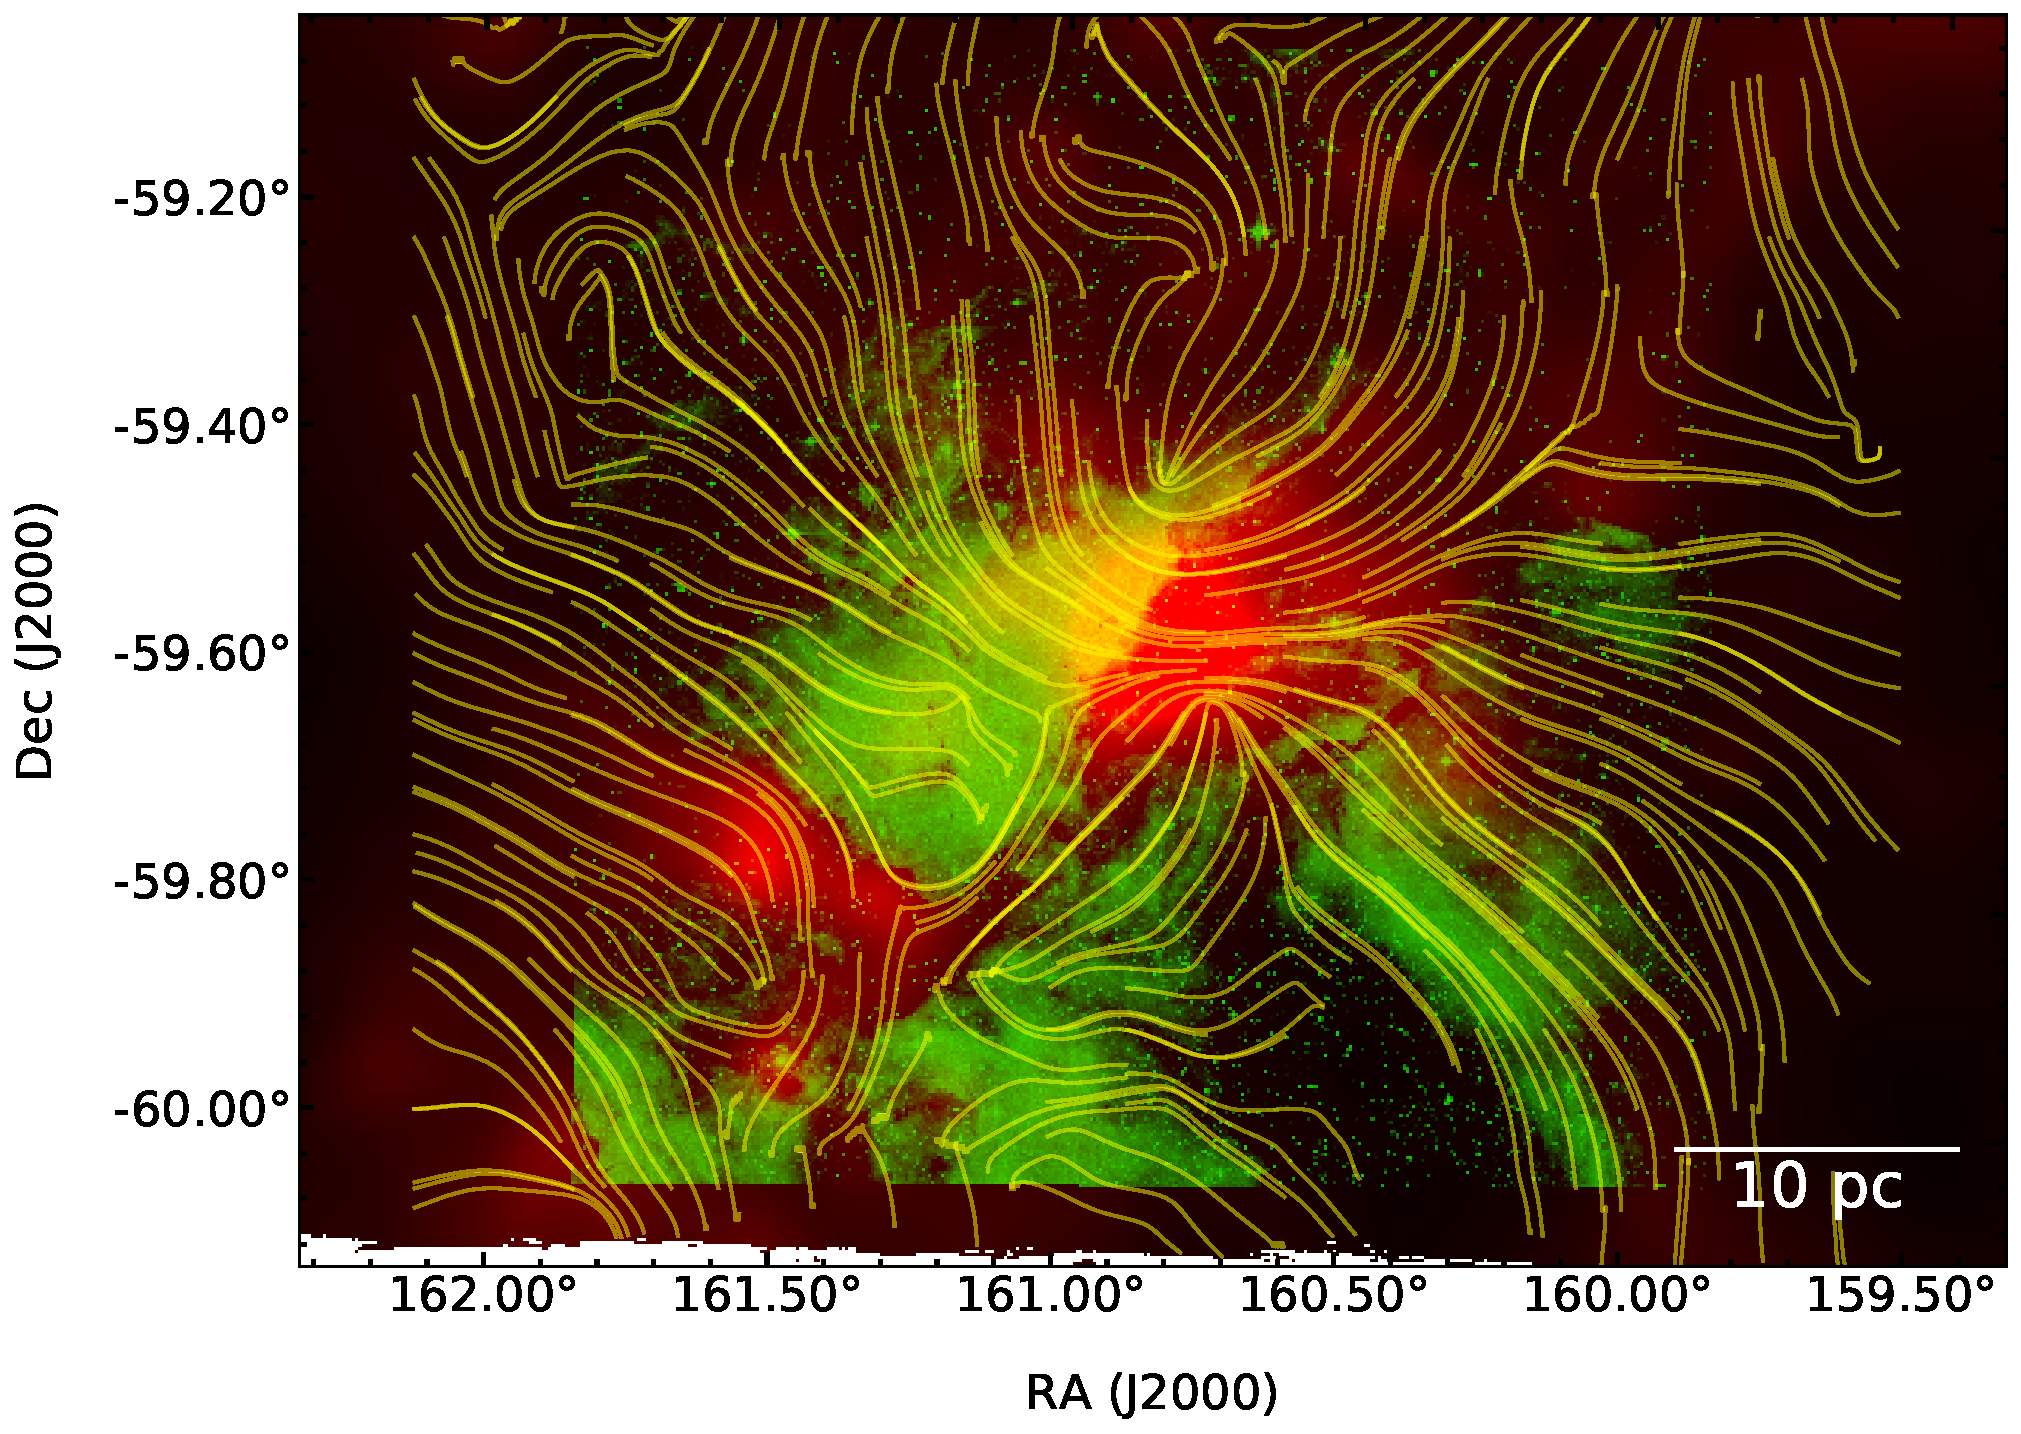
\includegraphics[width=\textwidth]{figures/carina/hstgsc2_250_sl}
\caption[An overlay of the GSC2 R-band CNC map (green) with a BLASTPol intensity map (red).]{An overlay of the GSC2 R-band CNC map (green) \citep{lasker2008second} with a BLASTPol intensity map (red). A subset of polarization vector streamlines are overplotted in yellow.}
\label{fig:hst_overplot}
\end{figure}

\begin{comment}
\begin{figure}[!htbp]
\centering
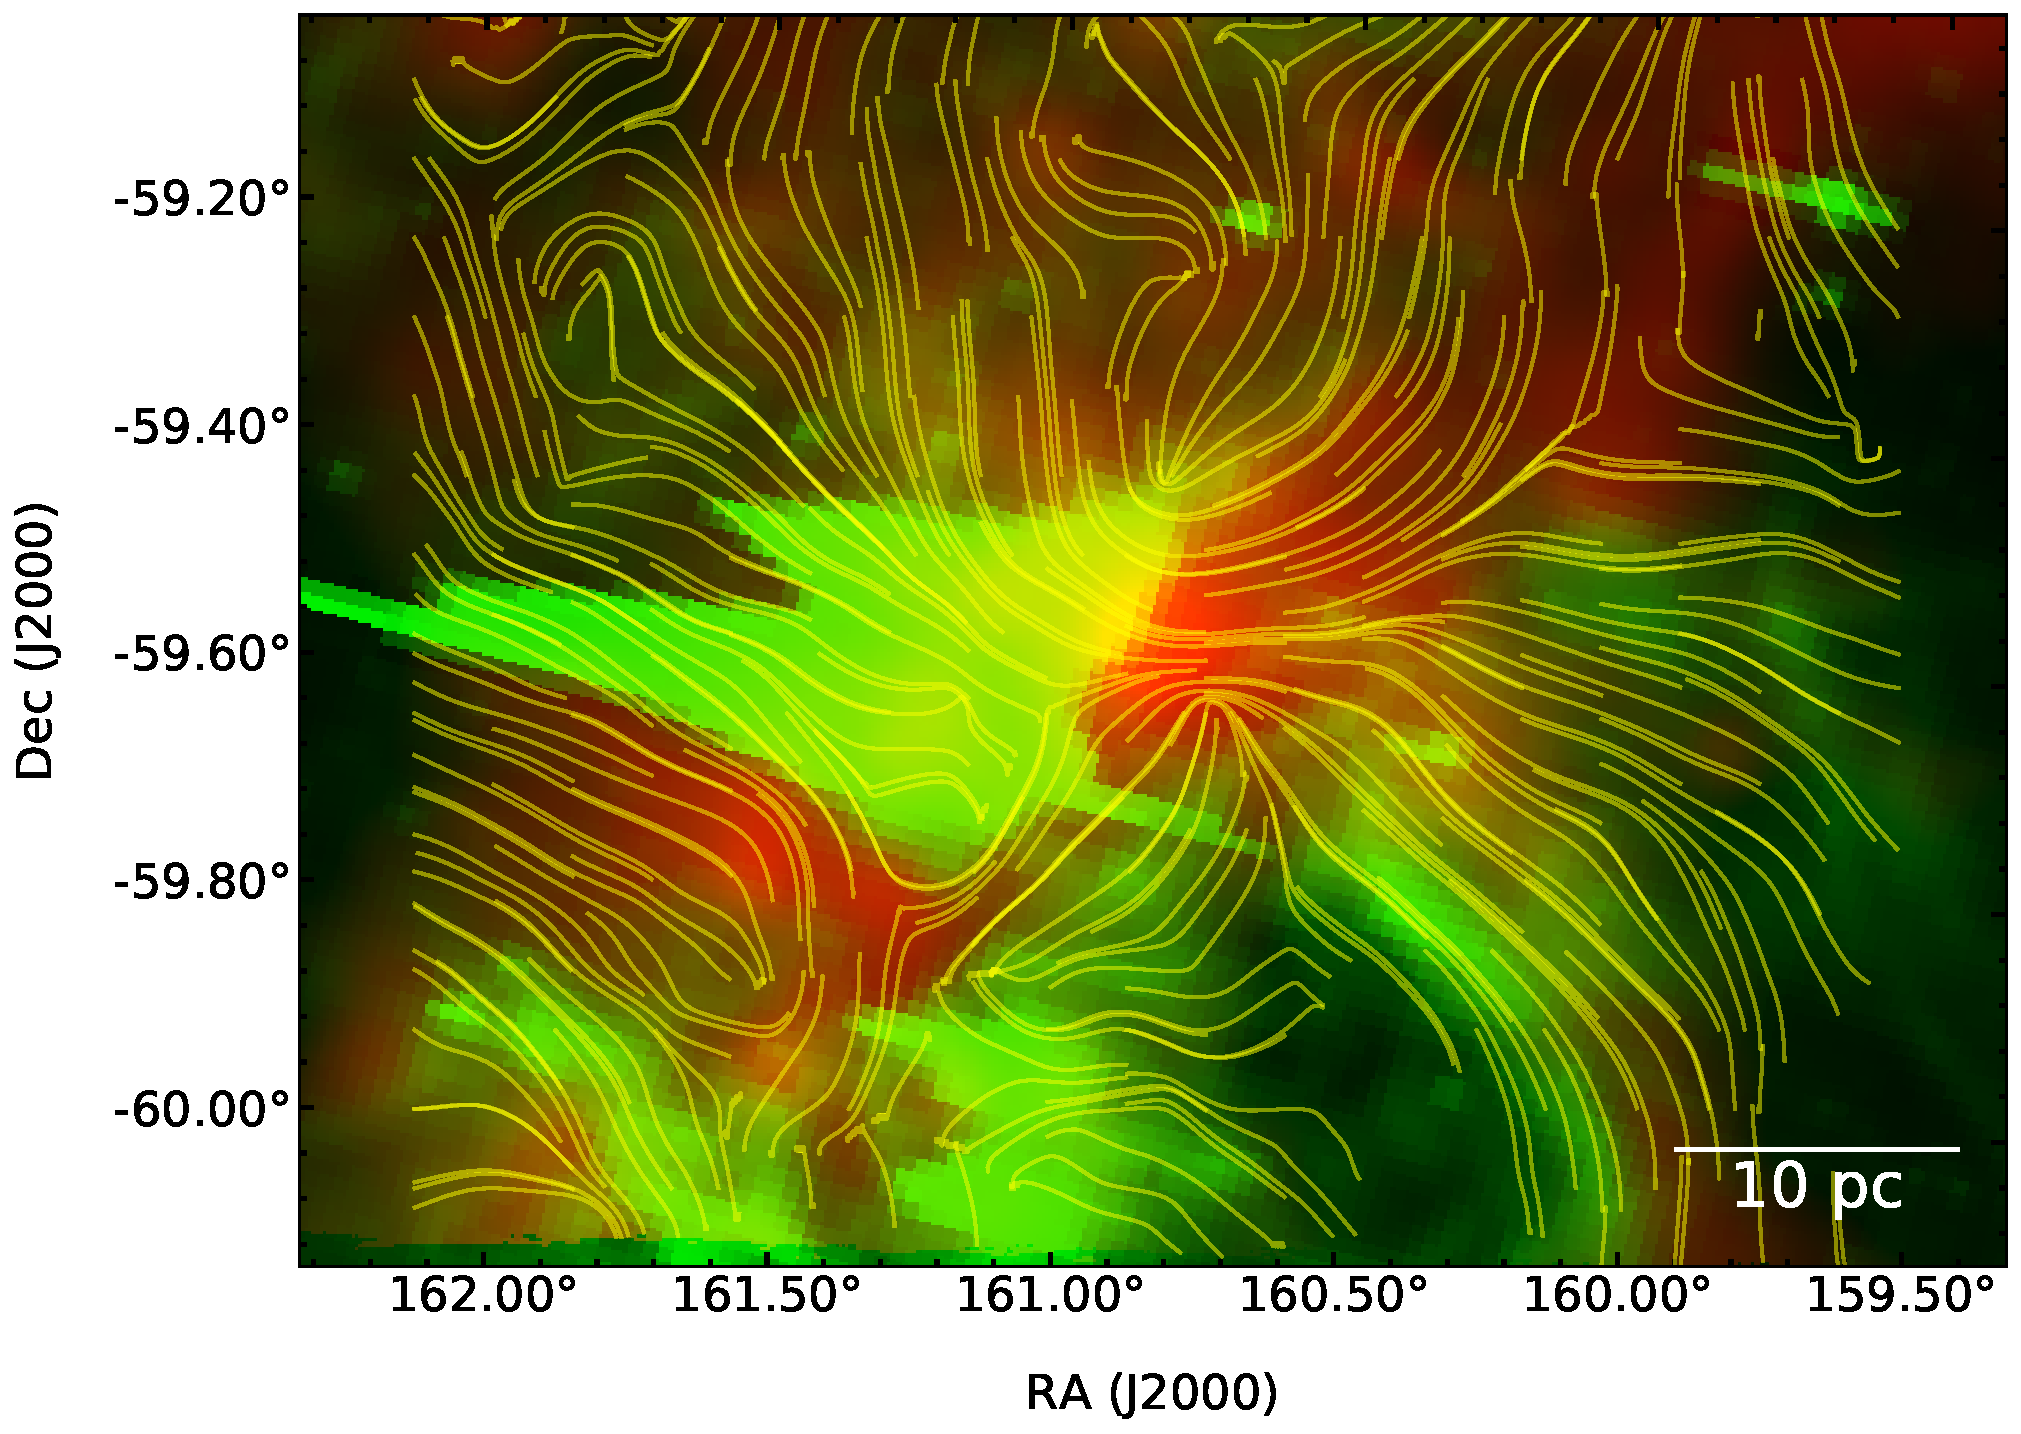
\includegraphics[width=\textwidth]{figures/carina/shassa32_sl}
\caption[An overlay of the SHASSA \macrocapwrap{H$\alpha$} CNC map (green) with a BLASTPol intensity map (red).]{An overlay of the SHASSA H$\alpha$ CNC map (green) \citep{gaustad2001robotic} with a BLASTPol intensity map (red). A subset of polarization vector streamlines are overplotted in yellow.}
\label{fig:shassa_overplot}
\end{figure}
\end{comment}

\begin{figure}[!htbp]
\centering
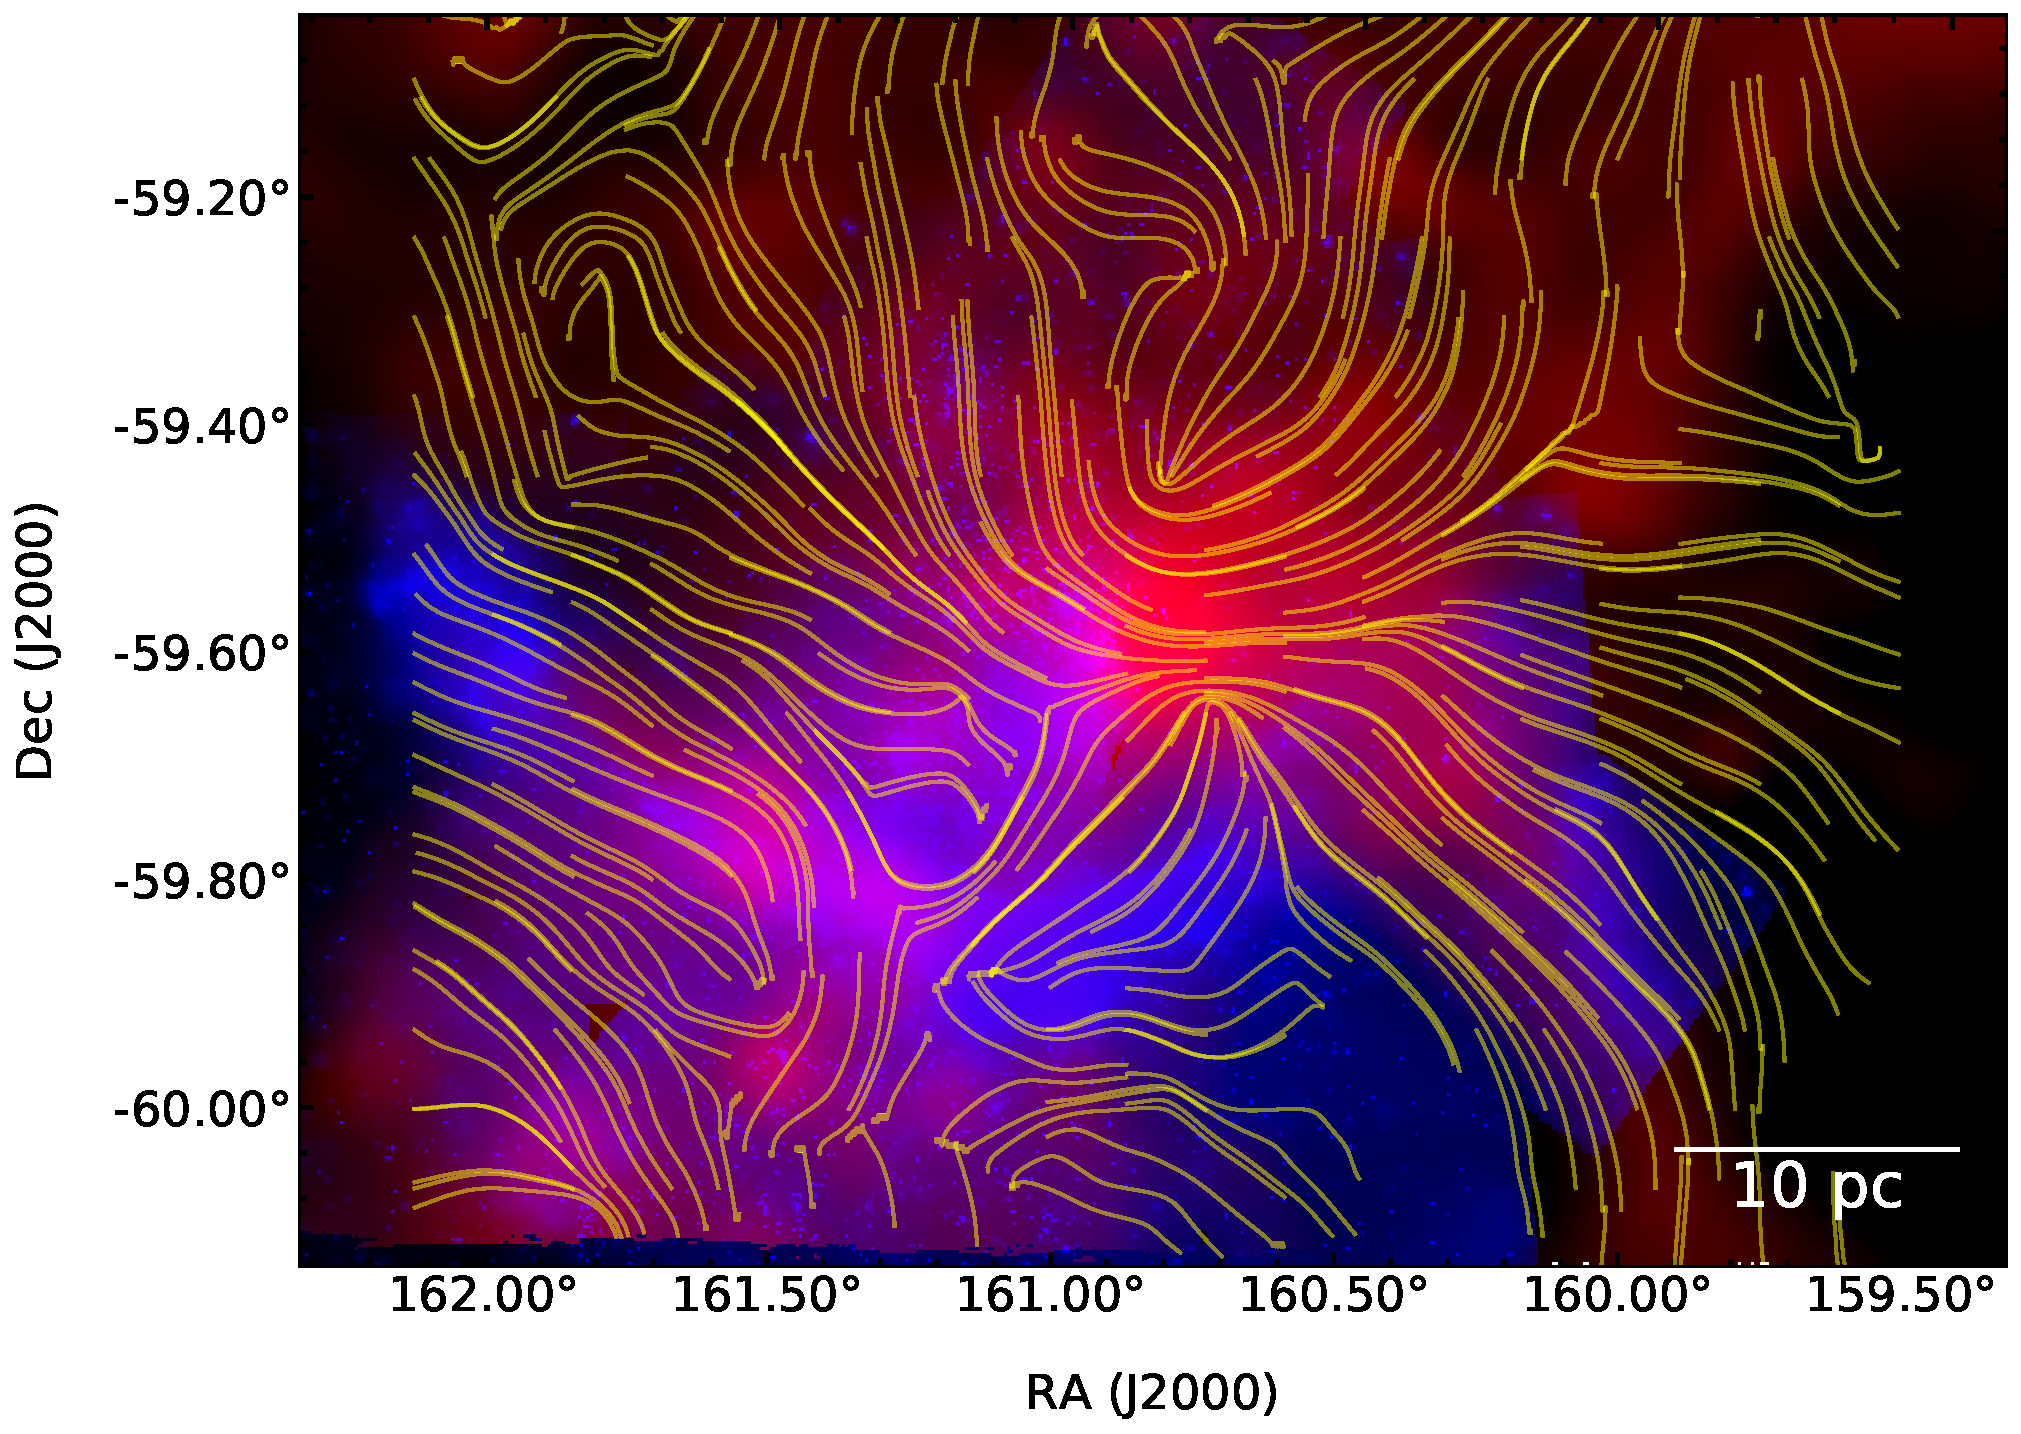
\includegraphics[width=\textwidth]{figures/carina/chandra_soft_sl}
\caption[An overlay of the Chandra soft-X-ray CNC map (blue) and BLASTPol intensity map (red).]{An overlay of the Chandra soft-X-ray CNC map (blue) \citep{townsley2011introduction} and BLASTPol intensity map (red). A subset of polarization vector streamlines are overplotted in yellow.}
\label{fig:chandra_overplot}
\end{figure}

\section{Estimating \macrocapwrap{\gls{Bpos}} using the DCFM}\label{DCFM}

In this section we apply a modified version of the Davis-Chandrasekhar-Fermi Method (DCFM) to the BLASTPol CNC map in order to estimate \gls{Bpos} along various sightlines through the complex. The DCFM is a technique which was first used by Chandrasekhar and Fermi to estimate \gls{Bpos} in the Orion spiral arm of the Milky Way (\citet{davis1951strength,chandrasekhar1953magnetic}). Using their method, they accurately estimated \gls{Bpos} at a level of a few~$\upmu$G. Although the estimates of \gls{Bpos} which are produced by the DCFM are known to carry inherent uncertainties of at least a factor of 2 (see Section~\ref{DCFM limitations}), it represents the most practical method of gaining insight into \gls{Bpos}, as it requires only a map of polarization vectors, and a map of the LOS velocity dispersion in an optically thin emission line.

\subsection{Description of the DCFM}

A magnetized plasma, such as that found throughout the ISM, supports transerve magnetohydrodynamic (MHD) waves known as Alfv$\acute{e}$n waves. Alfv$\acute{e}$n waves are  oscillations in the plasma which is frozen into the B-field. They're driven by the restorative force associated with the magnetic tension, $B^{2}/4\pi$ ($B^{2}/\mu_{0}$, in SI units), and propagate with a phase velocity (the Alfv$\acute{e}$n velocity) of:

\begin{equation}\label{eq:Alfven velocity}
  \gls{vA} = \frac{B}{\sqrt{4 \pi \rho}}
\end{equation}

where $\rho$ is the mass density of ionized material, and Equation~\ref{eq:Alfven velocity} is in CGS units. If $\rho$ can be estimated along a sightline of interest where there is a uniform B-field of magnitude $B_{0}$, then all that is needed to estimate $B_{0}$ is knowledge of $v_{A}$. To estimate $v_{A}$ using the DCFM relies on the assumption that the gas (ionized and neutral) and dust along the sightline are flux-frozen into $B_{0}$, so that any transverse spatial deviation of the material from the direction of $B_{0}$ can be attributed to an Alfv$\acute{e}$n wave. Ultimately, the spatial deviation is quantified using the dispersion of E-field polarization angles (see below). For $B_{0}$ oriented along the $z$-axis, and the LOS being the $x$-direction, the spatial deviation along the $y$-axis, is:

\begin{equation}\label{eq:y DCFM}
  y(x,t) \propto \mathrm{\cos}{\left( k(x - v_{A}t) \right)}
\end{equation}

This assumption is not completely valid in cases where there are significant dynamical forces at play besides the B-field, such as supernovae shocks and ionization fronts associated with HII regions, or strong turbulence. Here, we must assume that the turbulence is sub-Alfv$\acute{e}$nic. Despite this shortcoming of the DCFM, it is still useful as a method of obtaining rough upper limits on \gls{Bpos}.

Taking Equation~\ref{eq:y DCFM} as valid, \gls{vA} and $y(x, t)$ can be written into a wave equation as:

\begin{equation}\label{eq:wave equation}
  v_{A}^{2} \bigg \langle \frac{dy}{dx}  \bigg \rangle ^{2} = \bigg \langle \frac{dy}{dt}  \bigg \rangle ^{2}
\end{equation}

It then remains to estimate $dy/dx$ and $dy/dt$. The DCFM approach to doing so is to assume that the total B-field in the region is the sum of both the ordered component $B_{0}$ and a turbulent component $B_{t}$ ($B_{\mathrm{tot}} = B_{0} + B_{t}$). The turbulent field represents disorder which is caused by turbulent motions in the gas and dust. If the gas pressure is sub-dominant to magnetic pressure, then following \citet{hildebrand2009dispersion}, $B_{t} \ll B_{0}$, and $ \frac{\langle B_{t}^{2} \rangle ^{1/2}}{ B_{0} } \approx \frac{ \delta B }{ B_{0} }$.

The ratio $\delta B/ B_{0}$ is proportional to both $dy/dx$ and $dy/dt$. In the DCFM model, the former term can be empirically determined by measuring the dispersion in E-field polarization angles \gls{Sphi}. The second term is determined by measuring the LOS velocity dispersion \gls{sigV} in an optically thin emission line. Substituting $S_{\Phi}$ and $\sigma_{v}$ for $dy/dx$ and $dy/dt$ in Equation~\ref{eq:wave equation}, and then solving for $B$ yields the principle DCFM equation:

\begin{equation}\label{eq:DCFM 1}
    \gls{Bpos} = Q \sqrt{4 \pi \rho}\frac{S_{\Phi}}{\sigma_{v}} \qquad \left[ G \right]
\end{equation}

where $Q$ is a scale factor which accounts for uncertainties in the measured quantities, as well as the assumptions upon which the method is based. $Q$ is generally set equal to 0.5, although in this work, we choose $Q = 0.1$ (see Section~\ref{DCFM limitations}).

More recent users of the DCFM have made slight modifications to Equation~\ref{eq:DCFM 1}. In this work we adopt the expression derived by \citet{hildebrand2009dispersion}, which is also applied by \citet{crutcher2004scuba} and \citet{franco2015tracing}. Parameterizing the polarization angle dispersion as $b \approx \sqrt{2 S^{2}_{\Phi}}$ \citep{houde2009dispersion}, and calculating the FWHM of the LOS velocity line as $\Delta V_{LOS} = \sqrt{8 \ln 2} \sigma_{V}$, the DCFM equation can be expressed as:

 \begin{equation}\label{eq:DCFM 2}
    \gls{Bpos} = 9.3 \left( \frac{2\gls{nH2}}{\text{cm}^{-3}}  \right)^{1/2} \left( \frac{\Delta V_{\mathrm{LOS}}}{\text{km s}^{-1}} \right)  \left(  \frac{b}{1^{\degree}}\right)^{-1} \qquad \left[ \upmu G \right]
 \end{equation}

\subsection{Determining \macrocapwrap{$S_{\Phi}$}}\label{pol disp}

The dispersion in polarization angles $S_{\Phi}$ is calculated according to the method described in \citet{ade2015planck}. This method has been applied in a recent study of BLASTPol 2012 map of the Vela-C MC \citep{fissel2016balloon}. The calculation of $S_{\Phi}$ is as follows.

For every $N$ pixels in the polarization angle map the $\Phi$ value at that pixel is compared to that of $P$ pixels which surround it in an annular radius of $R$ pixels. For this work, $N = 3$, $P = 12$ and $R = 15$ (corresponding to a diameter of 5$\arcmin$). For the $ith$ pixel, the first step in the calculation is to compare its polarization angle, $\Phi[i]$, with those of the pixels which surround it at a radius of $R$ pixels. The polarization dispersion between each pair of pixels is:

\begin{equation}
  S^{2}_{\Phi}[i,R] = \left( \Phi[i] - \Phi[i + R] \right)^{2}
\end{equation}

After calculating $S^{2}_{\Phi}[i,R]$ for each pair of pixels, the final polarization dispersion value $S^{2}_{\Phi}[i]$ is the average of the pairs:

\begin{equation}
  S^{2}_{\Phi}[i] = \frac{1}{N} \sum\limits_{i=0}^{N} S^{2}_{\Phi}[i]
\end{equation}

Following \citet{fissel2016balloon}, the values of $S$ which are used in the final DCFM calculations are debiased by subtracting the variance of $S^{2}_{\Phi}[i]$:

\begin{equation}\label{eq:ADF}
  S_{\Phi,\mathrm{db}} = \sqrt{S_{\Phi}^{2} - \sigma^{2}_{S_\Phi}}
\end{equation}

A histogram of \gls{Phi} calculated along $\sim$165,000 sightlines corresponding to the inner $\sim$1.25~deg$^{2}$ of the CNC is shown in Figure~\ref{fig:S_hist}, and a histogram of \gls{Sphi} for $\sim$33,000 sightlines within the same region is shown in Figure~\ref{fig:S_hist}. First and second moments for both quantities are reported in Table~\ref{table:S_and_Phi}. We find that in the inner region of the CNC, $\langle \gls{Sphi} \rangle \approx 20$~deg.

In Figure~\ref{fig:Phi_hist}, the polarization angles are reported relative to Galactic coordinates, where 90~deg corresponds to \gls{Bpos} parallel to the GP\@. We find that $\langle \gls{Phi} \rangle = 96$~deg, and that 50\% of the B-field polarization angles are within $\pm$ 23~deg of the GP\@. This finding agrees with \citet{li2006results}, which reports $\langle \Phi \rangle \leq 15$~deg of the GP for three GMCs, including the CNC\@.

\begin{table}[!htbp]
\centering
\begin{tabular}{@{}llll@{}}
\dtoprule{}
 & N$_{\mathrm{sl}}$ & Mean (deg) & $\sigma$ (deg) \\ \midrule
$\Phi$  & 165,000 & 96 & 33 \\
$S_{\phi}$  & 33,000 & 20 & 26 \\ \dbottomrule{}
\\
\end{tabular}
\caption[First and second moments of the \macrocapwrap{\gls{Phi}} and \macrocapwrap{\gls{Sphi}} distribution over the inner \macrocapwrap{$\sim$1.25~deg$^{2}$} of the CNC.]{First and second moments of the \gls{Phi} and \gls{Sphi} distribution over the inner $\sim$1.25~deg$^{2}$ of the CNC\@. $N_{\mathrm{sl}}$ is the number of sightlines reported.}
\label{table:S_and_Phi}
\end{table}

\begin{figure}[!htbp]
\centering
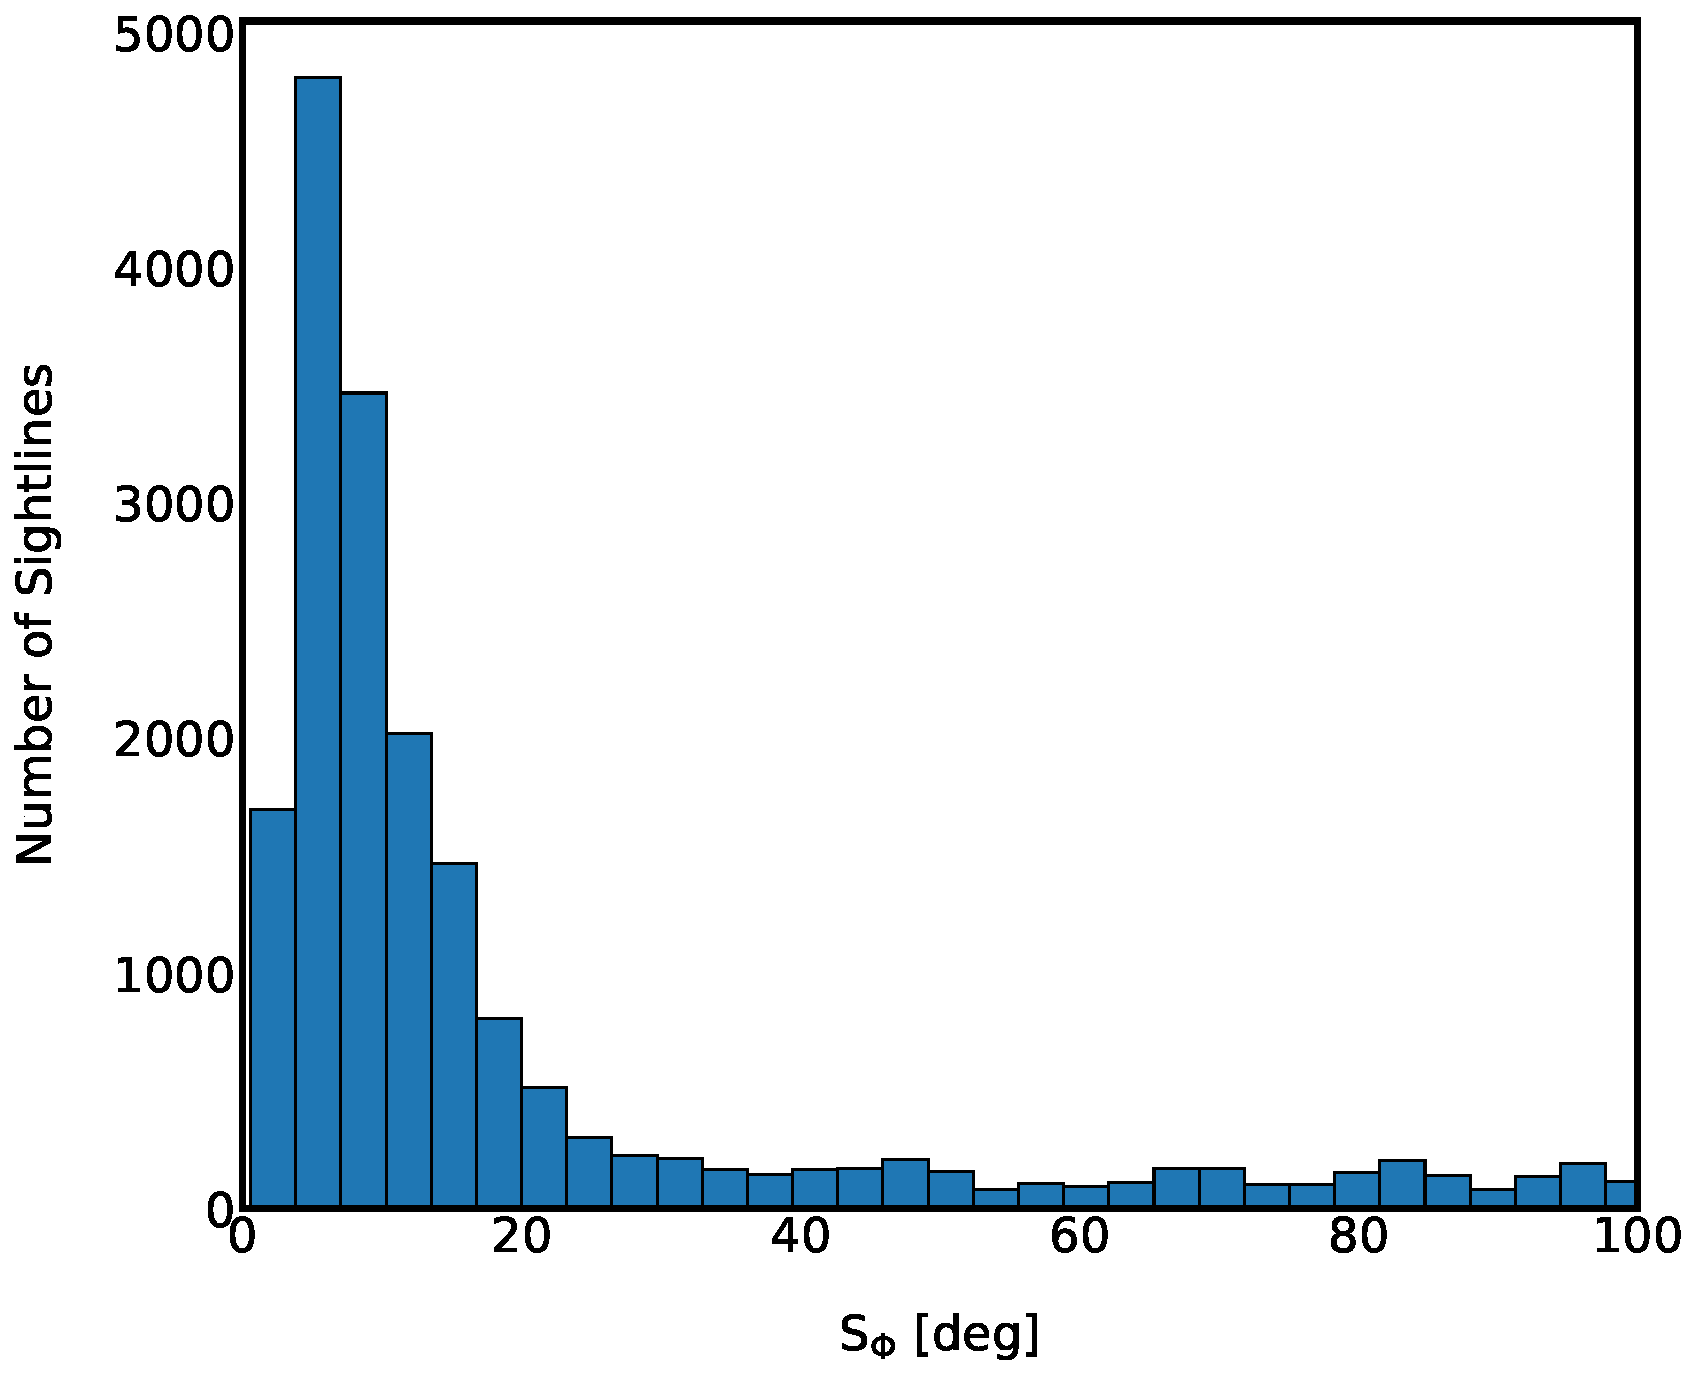
\includegraphics[width=\textwidth]{figures/carina/S_hist}
\caption[A histogram of the dispersion in polarization angle.]{A histogram of \gls{Sphi}, the polarization angle dispersion (deg).}
\label{fig:S_hist}
\end{figure}

\begin{figure}[!htbp]
\centering
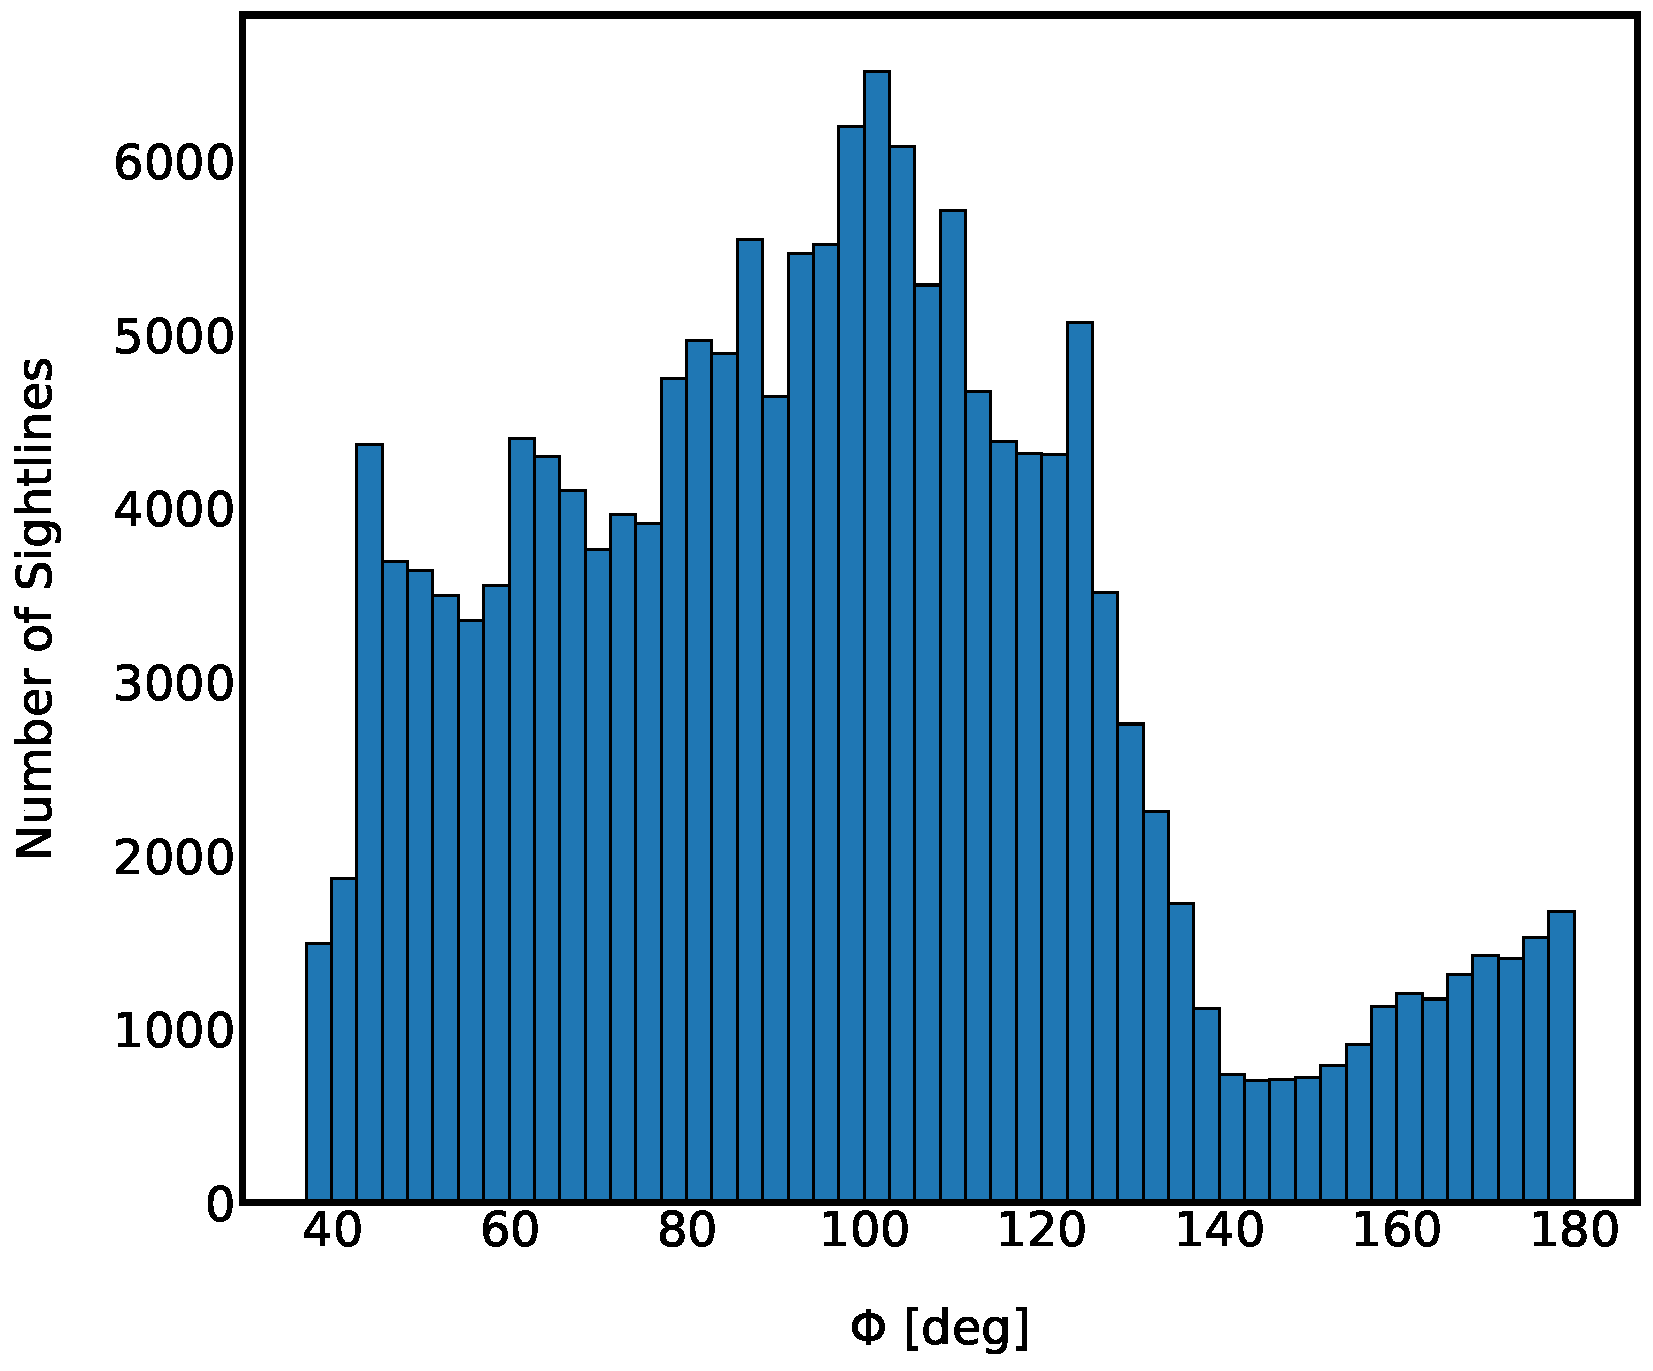
\includegraphics[width=\textwidth]{figures/carina/Phi_hist}
\caption[A histogram of the polarization angle.]{A histogram of \gls{Phi} (deg), where 90~deg is parallel to the GP.}
\label{fig:Phi_hist}
\end{figure}

\subsection{Determining \macrocapwrap{\gls{nH2}}}\label{nh2}

To determine the number density of molecular hydrogen \gls{nH2} which is needed to compute \gls{Bpos} using Equation~\ref{eq:DCFM 2}, we first calculate the column density of molecular hydrogen \gls{NH2}. The column density can be computed from the total intensity maps at each of the three BLASTPol bands as:

\begin{equation}\label{eq:NH2}
  \gls{NH2} = 2\frac{ \tau_{\nu} R}{\kappa_{\nu} m_{H_2}} \qquad \left[ \text{cm}^{-2} \right]
\end{equation}

where:
\begin{itemize}[label={},nosep]
  \item $\tau_{\nu}$ is the optical depth at frequency $\nu$
  \item $R = 100$ is the gas-to-dust mass ratio
  \item $\kappa_{\nu}$ is the dust opacity at frequency $\nu$ [cm$^{2}$/g]
  \item $m_{H_2}$ = 3.32 $\times$ $10^{-24}$ is the mass of molecular hydrogen [g]
\end{itemize}

The FIR dust opacity \gls{kappa} is calculated using the empirical relation found in \citet{mathis1990interstellar}:

\begin{equation}\label{eq:kappa}
  \kappa_{\nu} = \kappa_{\lambda} = 13.6 (\lambda / 250 \mathrm{\upmu m})^{-2} \qquad \left[ \mathrm{cm}^{2}/\mathrm{g} \right]
\end{equation}

and the optical depth at frequency $\nu$ is:

\begin{align}\label{eq:tau}
  \tau_{\nu} &= \frac{F_{\nu}\Omega_{\mathrm{beam}}}{B_{\nu}(T_{d})} \\
          &= \frac{I_{\nu}}{B_{\nu}(T_{d})} \\
\end{align}

where $B_{\nu}(T_{d})$ is the Planck function, and $T_{d}$ is the dust temperature, taken from the Planck 353~GHz map of the CNC, and re-gridded to the BLASTPol map coordinates.

Once \gls{NH2} is known, the total visual extinction \gls{AV} can be calculated using the canonical relation described in \citet{bohlin224savage}:

\begin{equation}\label{eq:Av}
A_{V} = \frac{ 9.4 \times 10^{20}}{\gls{NH2}} \qquad \left[ \mathrm{mag} \right]
\end{equation}

Mean values for optical depth $\tau_{\nu}$, dust opacity $\kappa_{\nu}$, molecular hydrogen column density \gls{NH2}, and total visual extinction \gls{AV} are listed in Table~\ref{table:NH2_fit} for the inner $\sim$1.25~deg$^{2}$ of the CNC\@. The quantities are calculated for each of the three BLASTPol bands. A histogram of \gls{NH2}, taken over the same region, is shown in Figure~\ref{fig:NH2_hist}. The values for \gls{NH2} and \gls{AV} agree with those presented in \citet{preibisch2012herschel}. It should be noted that the dust opacities (Equation~\ref{eq:kappa}) carry an uncertainty of a factor of $\sim$2, which translates into an uncertainty in \gls{NH2}.


\begin{table}[!htbp]
  \centering
\begin{tabular}{@{}llll@{}}
\dtoprule{}
      & 250~$\upmu$m                              & 350~$\upmu$m       & 500~$\upmu$m              \\ \midrule
$\langle \tau_{\nu}  \rangle$  & 2.09 $\times$ 10$^{-3}$ & 2.06 $\times$ 10$^{-4}$ & 3.1 $\times$ 10$^{-3}$  \\
$\kappa_{\nu}$ ($\mathrm{cm}^{2}/\mathrm{g}$)    & 13.16             & 4.06     & 3.29                    \\
$\langle \gls{NH2}  \rangle$  ($\mathrm{cm}^{-2}$) & 2.09 $\times$ 10$^{21}$                 & 4.5 $\times$ 10$^{21}$                 & 2.88 $\times$ 10$^{21}$ \\
$\langle A_{V} \rangle$  ($\mathrm{mag}$)                              & 3.03                   & 2.06                   & 1.03                    \\ \dbottomrule{}
\\
\end{tabular}
\centering
\caption[Estimated map parameters calculated using total intensity maps over the inner \macrocapwrap{$\sim$1.25~deg$^{2}$} of the CNC.]{The mean values of optical depth $\tau_{\nu}$, dust opacity $\kappa_{\nu}$, molecular hydrogen column density \gls{NH2} and total visual extinction \gls{AV} calculated with the $I_{250}$, $I_{350}$ and $I_{500}$ maps for the inner $\sim$1.25~deg$^{2}$ of the CNC.}
\label{table:NH2_fit}
\end{table}

% NH2 histogram
\begin{figure}[!htbp]
\centering
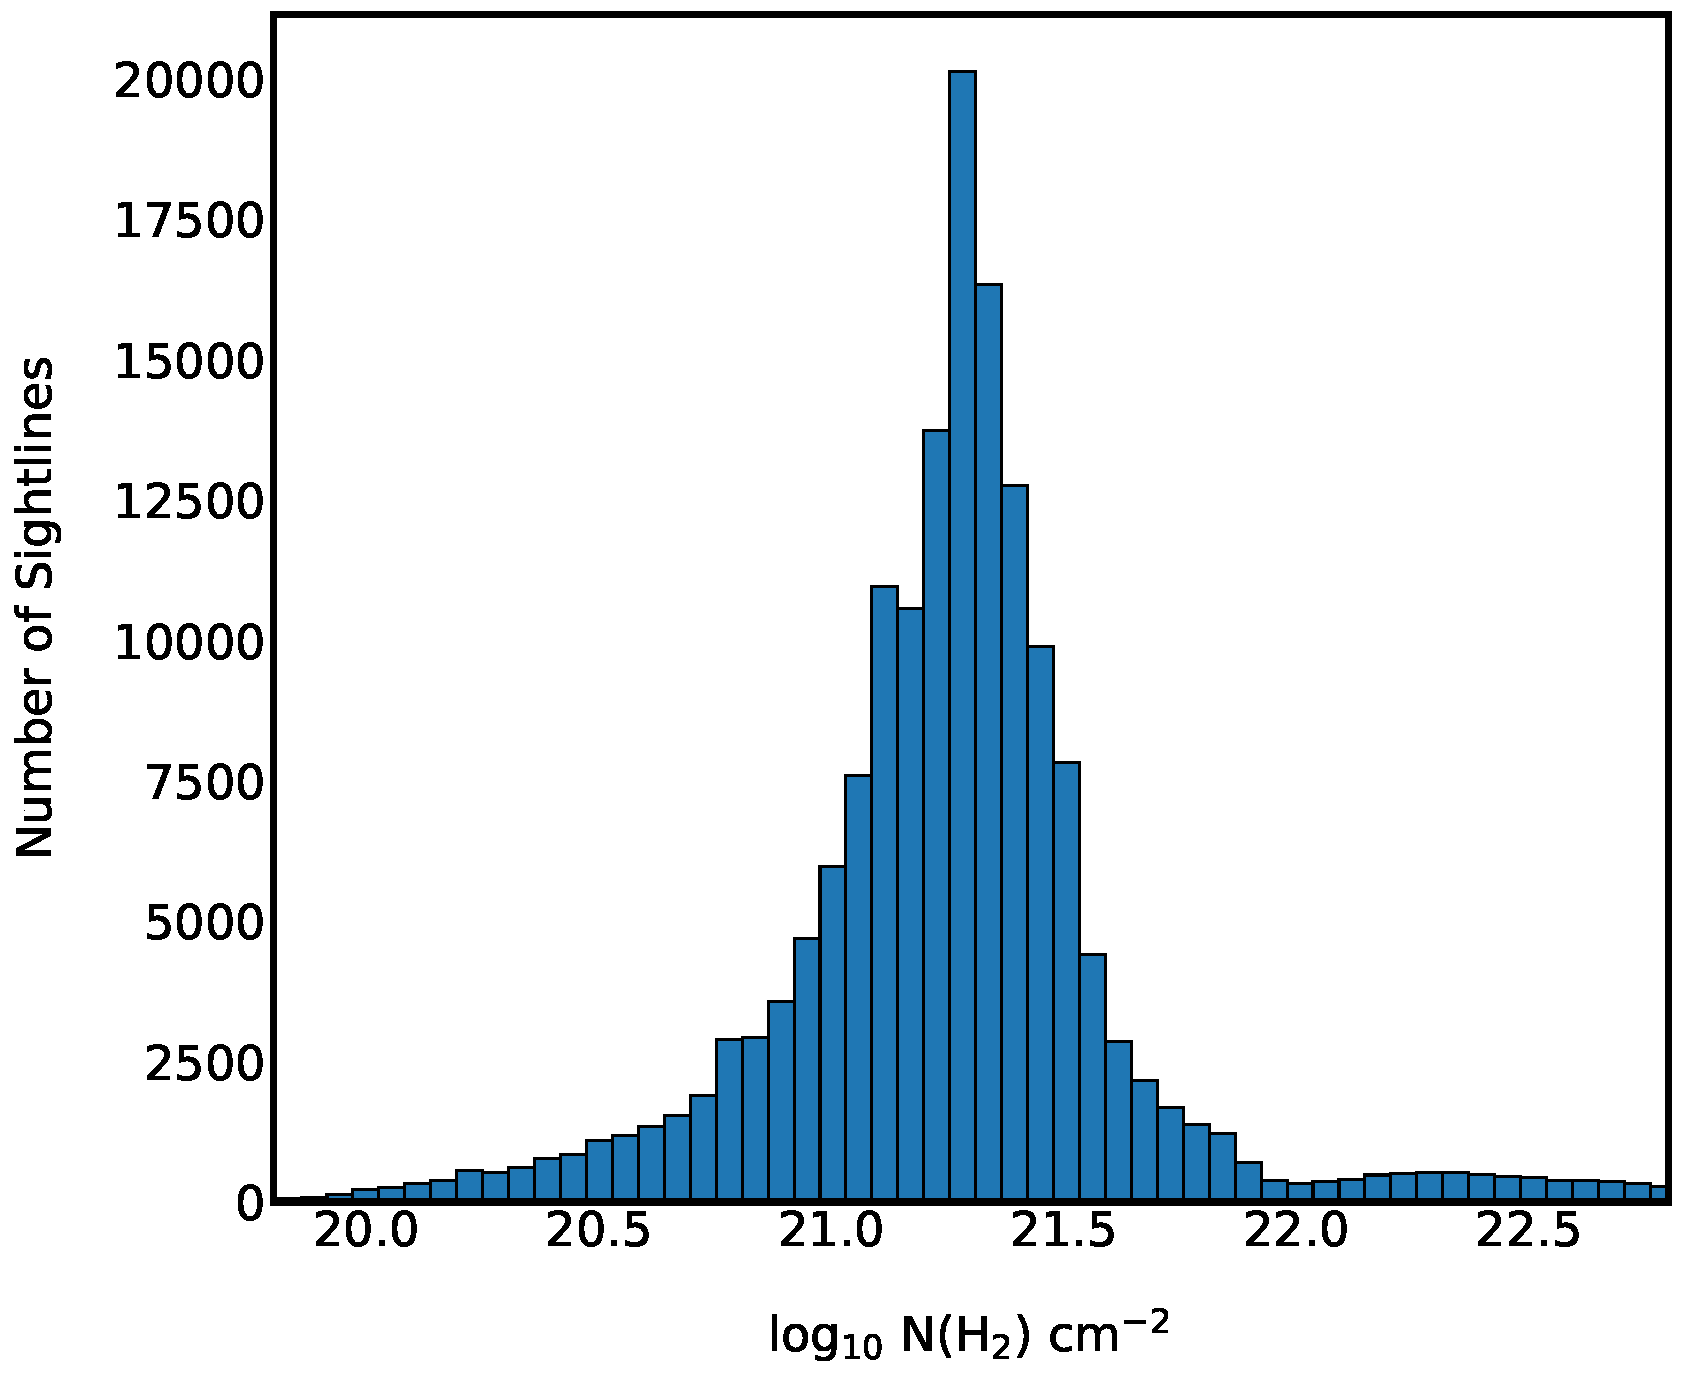
\includegraphics[width=\textwidth]{figures/carina/NH2_hist_500}
\caption[A histogram of \macrocapwrap{\gls{NH2}} over the inner \macrocapwrap{$\sim$1.25~deg$^{2}$} of the CNC.]{A histogram of \gls{NH2} over the inner $\sim$1.25~deg$^{2}$ of the CNC.}
\label{fig:NH2_hist}
\end{figure}

% nH2 histogram
\begin{figure}[!htbp]
\centering
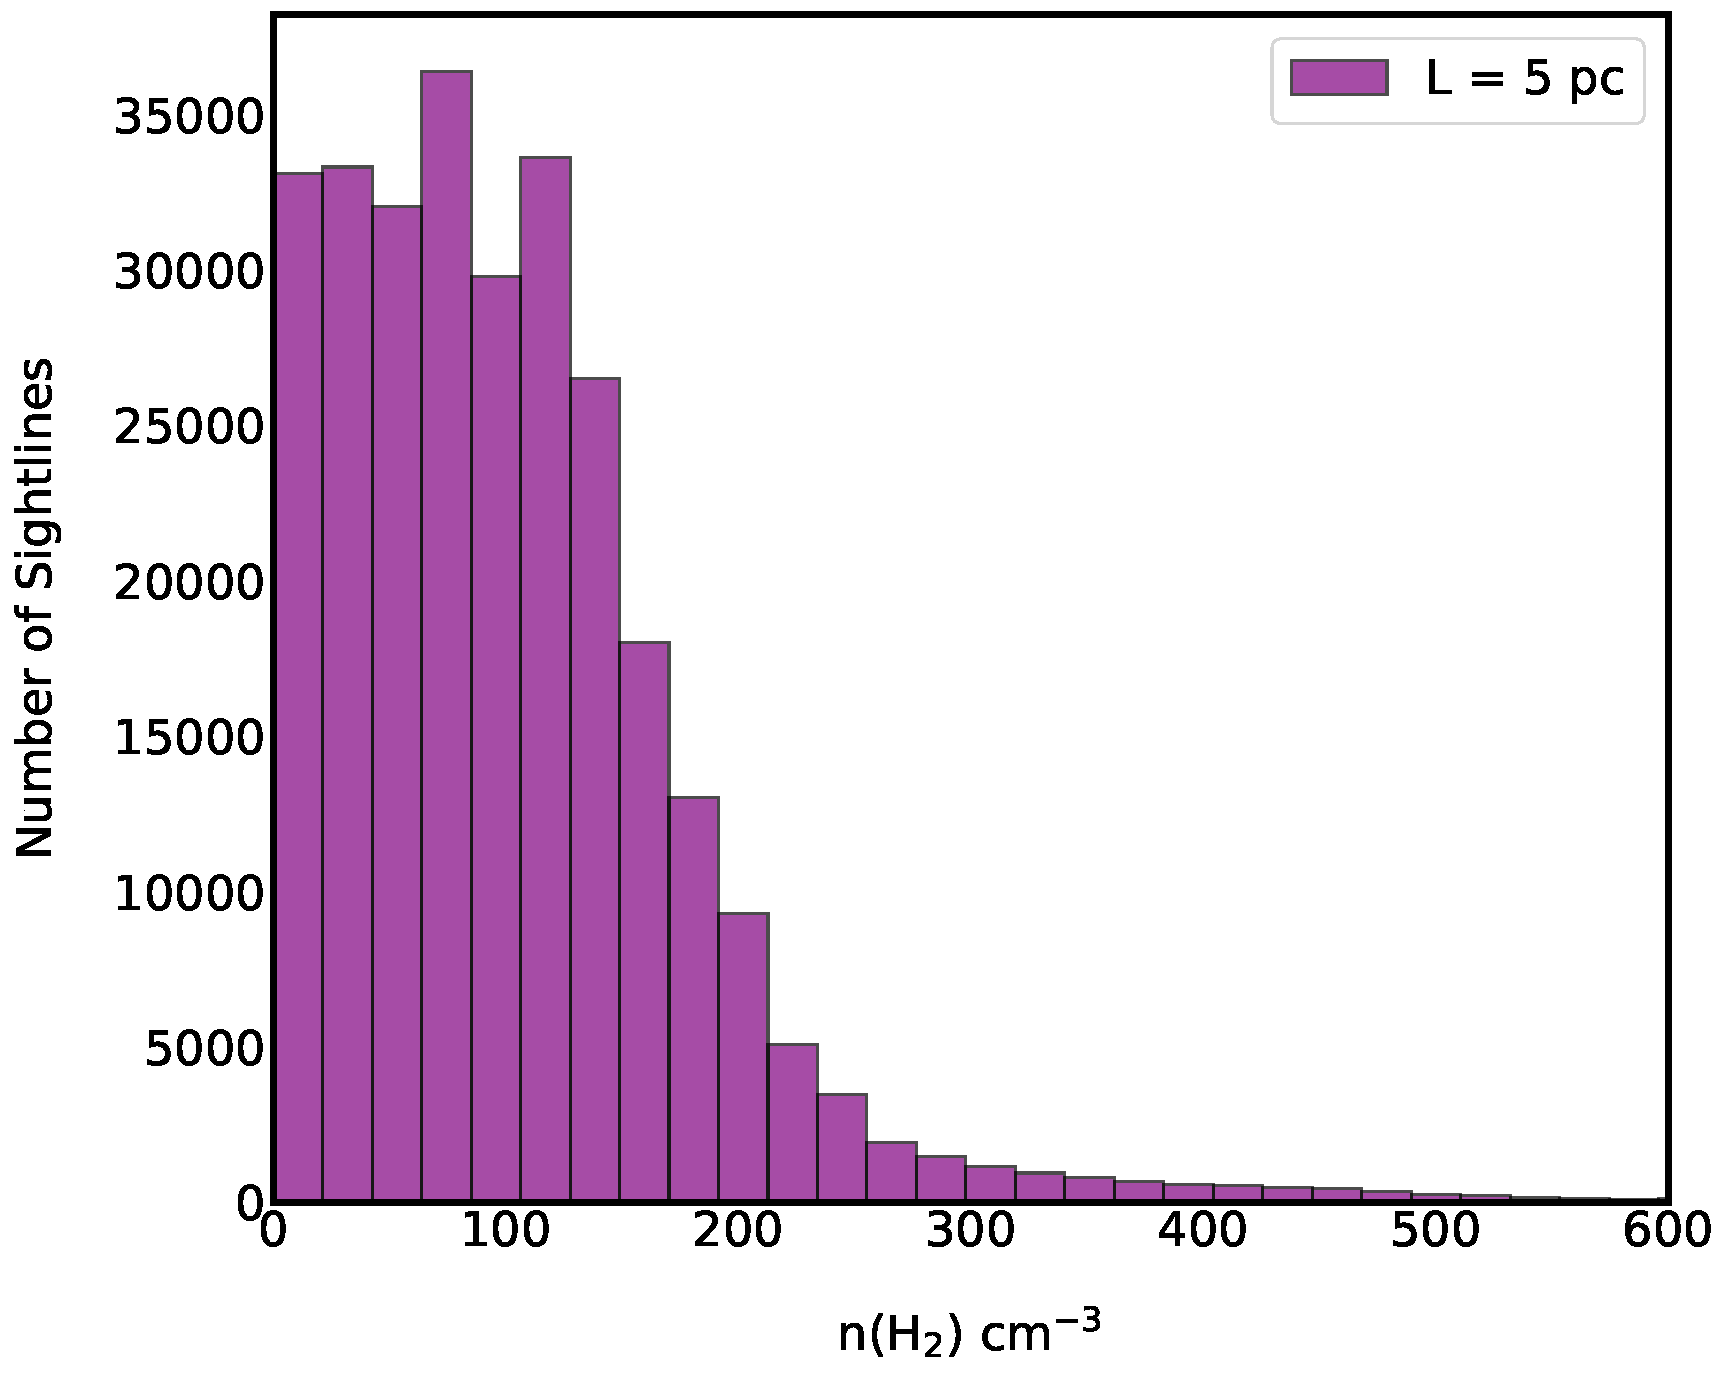
\includegraphics[width=\textwidth]{figures/carina/nH2_hist_500}
\caption[A histogram of \macrocapwrap{\gls{nH2}} in the inner \macrocapwrap{$\sim$1.25~deg$^{2}$} of the CNC.]{A histogram of \gls{nH2} in the inner $\sim$1.25~deg$^{2}$ of the CNC, shown for an assumed column depth of 5~pc.}
\label{fig:nH2_hist}
\end{figure}

To calculate \gls{nH2}, we must assume a column depth through the CNC\@. The complex morphology of the region makes it infeasible to assign a single column depth to the entire map. Instead, we examine a range of \gls{nH2}, which extends over an order of magnitude: $0.5 \text{~pc} \leq L_{\mathrm{CNC}} \leq 5 \text{~pc}$. The mean and maximum values of \gls{nH2} corresponding to these two limits are listed in Table~\ref{table:nH2}, for the each of the three BLASTPol bands. A histogram of the \gls{nH2} values corresponding to $L_{\mathrm{CNC}} = 5$~pc is shown in Figure~\ref{fig:nH2_hist}.

\begin{table}[hbtp]
  \centering
\begin{tabular}{@{}llll@{}}
\dtoprule{}
                            & 250~$\upmu$m     & 350~$\upmu$m     & 500~$\upmu$m     \\ \midrule
$\langle \gls{nH2} \rangle$ ($\mathrm{cm}^{-3}$) & 93--930      & 94--941      & 133--1330    \\
max \gls{nH2} ($\mathrm{cm}^{-3}$)             & 4,837--48,370 & 3645--36,450 & 4,008--40,080
\\ \dbottomrule{}
\\
\end{tabular}
\centering
\caption[Mean and maximum values of \macrocapwrap{\gls{nH2}} shown for each BLASTPol band.]{Mean and maximum values of \gls{nH2} shown for each BLASTPol band. The lower and upper ranges correspond to column depths $L_{\mathrm{CNC}}$ of 0.5~pc and 5~pc.}
\label{table:nH2}
\end{table}

\subsection{Determining \macrocapwrap{$\sigma_{v}$}}\label{sigV}

To estimate \gls{Bpos} using Equation~\ref{eq:DCFM 2} requires velocity dispersion values from an optically thin line which are sampled over the BLASTPol CNC field. It is also important that the spatial resolution of the velocity map is at least as high as the BLASTPol map. In this work, we use the $\mathrm{HI}$ 21~cm data cube of the CNC region acquired with the Australia Telescope Compact Array (ATCA) \citep{rebolledo2017carina}. The spatial coverage of the map contains the entire BLASTPol CNC region, and is taken at a resolution of $\sim$35$\arcsec$. In the following analysis, the $\mathrm{HI}$ data cube is smoothed to 5$\arcmin$ to match the resolution of the Planck maps. The ATCA observations probe a velocity range of $\sim$200~km/s, with a velocity resolution of $\sim$500~m/s.

After smoothing each slice of the ATCA data cube to 5$\arcmin$, the ROI is aligned with the BLASTPol map by converting its coordinates from the galactic to the equatorial frame. The resulting overlay is shown in Figure~\ref{fig:HI_vselect}. Once aligned, the average $\mathrm{HI}$ line profile along the velocity axis of the cube (i.e., into the plane of Figure~\ref{fig:HI_vselect}) is averaged around each map location which was used in the calculation of \gls{Sphi} (Section~\ref{pol disp}). A subset of these regions is shown in Figure~\ref{fig:HI_vselect}, highlighted in yellow.

Before calculating the velocity dispersion \gls{sigV} from each average line-profile, the profiles are low-pass filtered, and profiles containing spurious noise are removed from the set. The dispersion of each line profile is estimated by applying a curve fitting algorithm which produces Maximum Likelihood Estimates (MLEs) for the FWHM of a Gaussian profile. A histogram showing the distribution of $v_{\mathrm{FWHM}}$ for $\sim$30,000 lines of sight is shown in Figure~\ref{fig:vfwhm_hist}. The distribution of $v_{\mathrm{FWHM}}$ is roughly Gaussian, with a mean and standard deviation of $\sim$38 km/s and $\sim$5 km/s. A map of $v_{\mathrm{FWHM}}$ over the CNC region used in the DCFM analysis is shown in Figure~\ref{fig:vfwhm_map}, with \gls{Bpos} pseudovectors (Downsampled by 20x) overplotted in white.

\begin{figure}[!htbp]
\centering
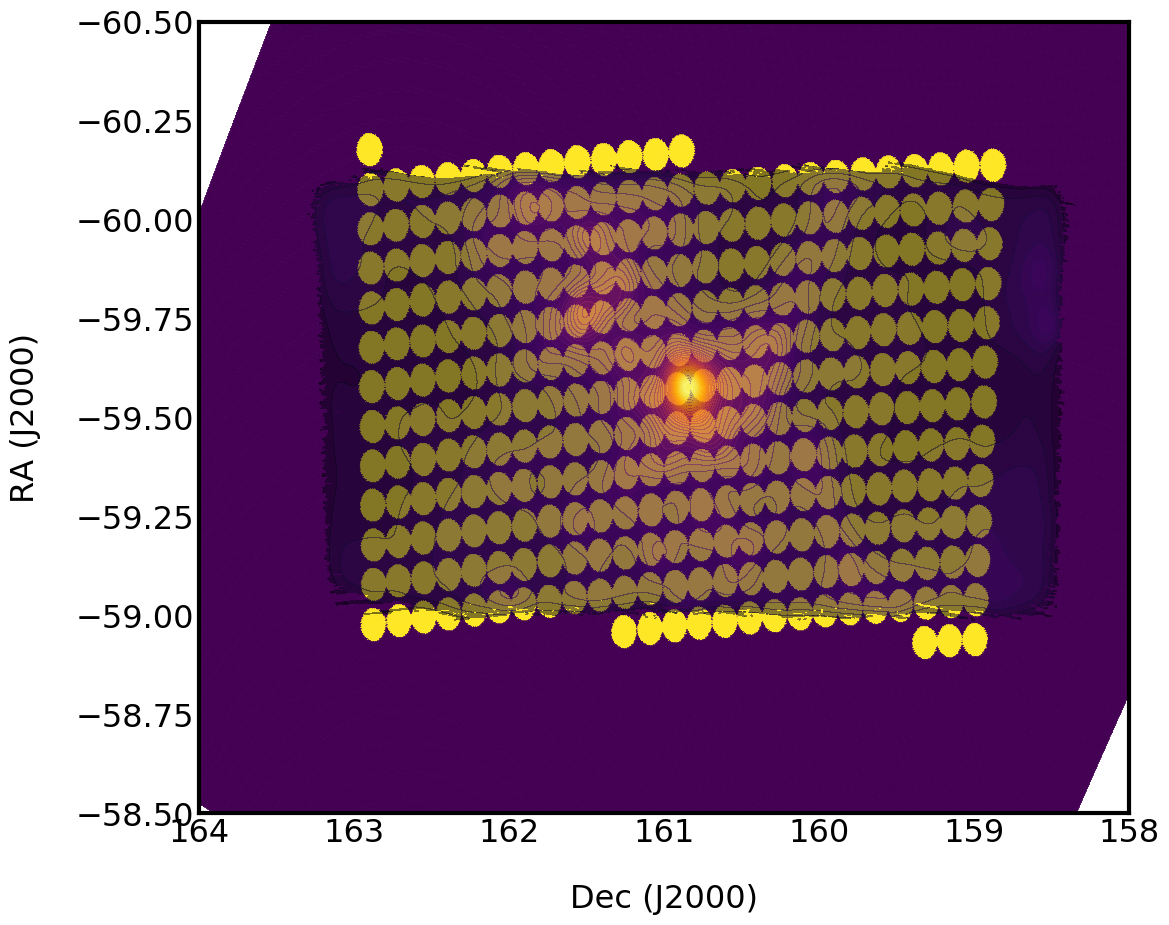
\includegraphics[width=\textwidth]{figures/carina/HI_vselect}
\caption[An overlay of one slice of the ATCA HI velocity cube with the BLASTPol intensity map.]{An overlay of one slice of the ATCA $\mathrm{HI}$ velocity cube with the BLASTPol intensity map. A subset of the regions used to calculate average HI line profiles are highlighted in yellow. The diameter of the regions is $\sim$5$\arcmin$.}
\label{fig:HI_vselect}
\end{figure}

\begin{figure}[!htbp]
\centering
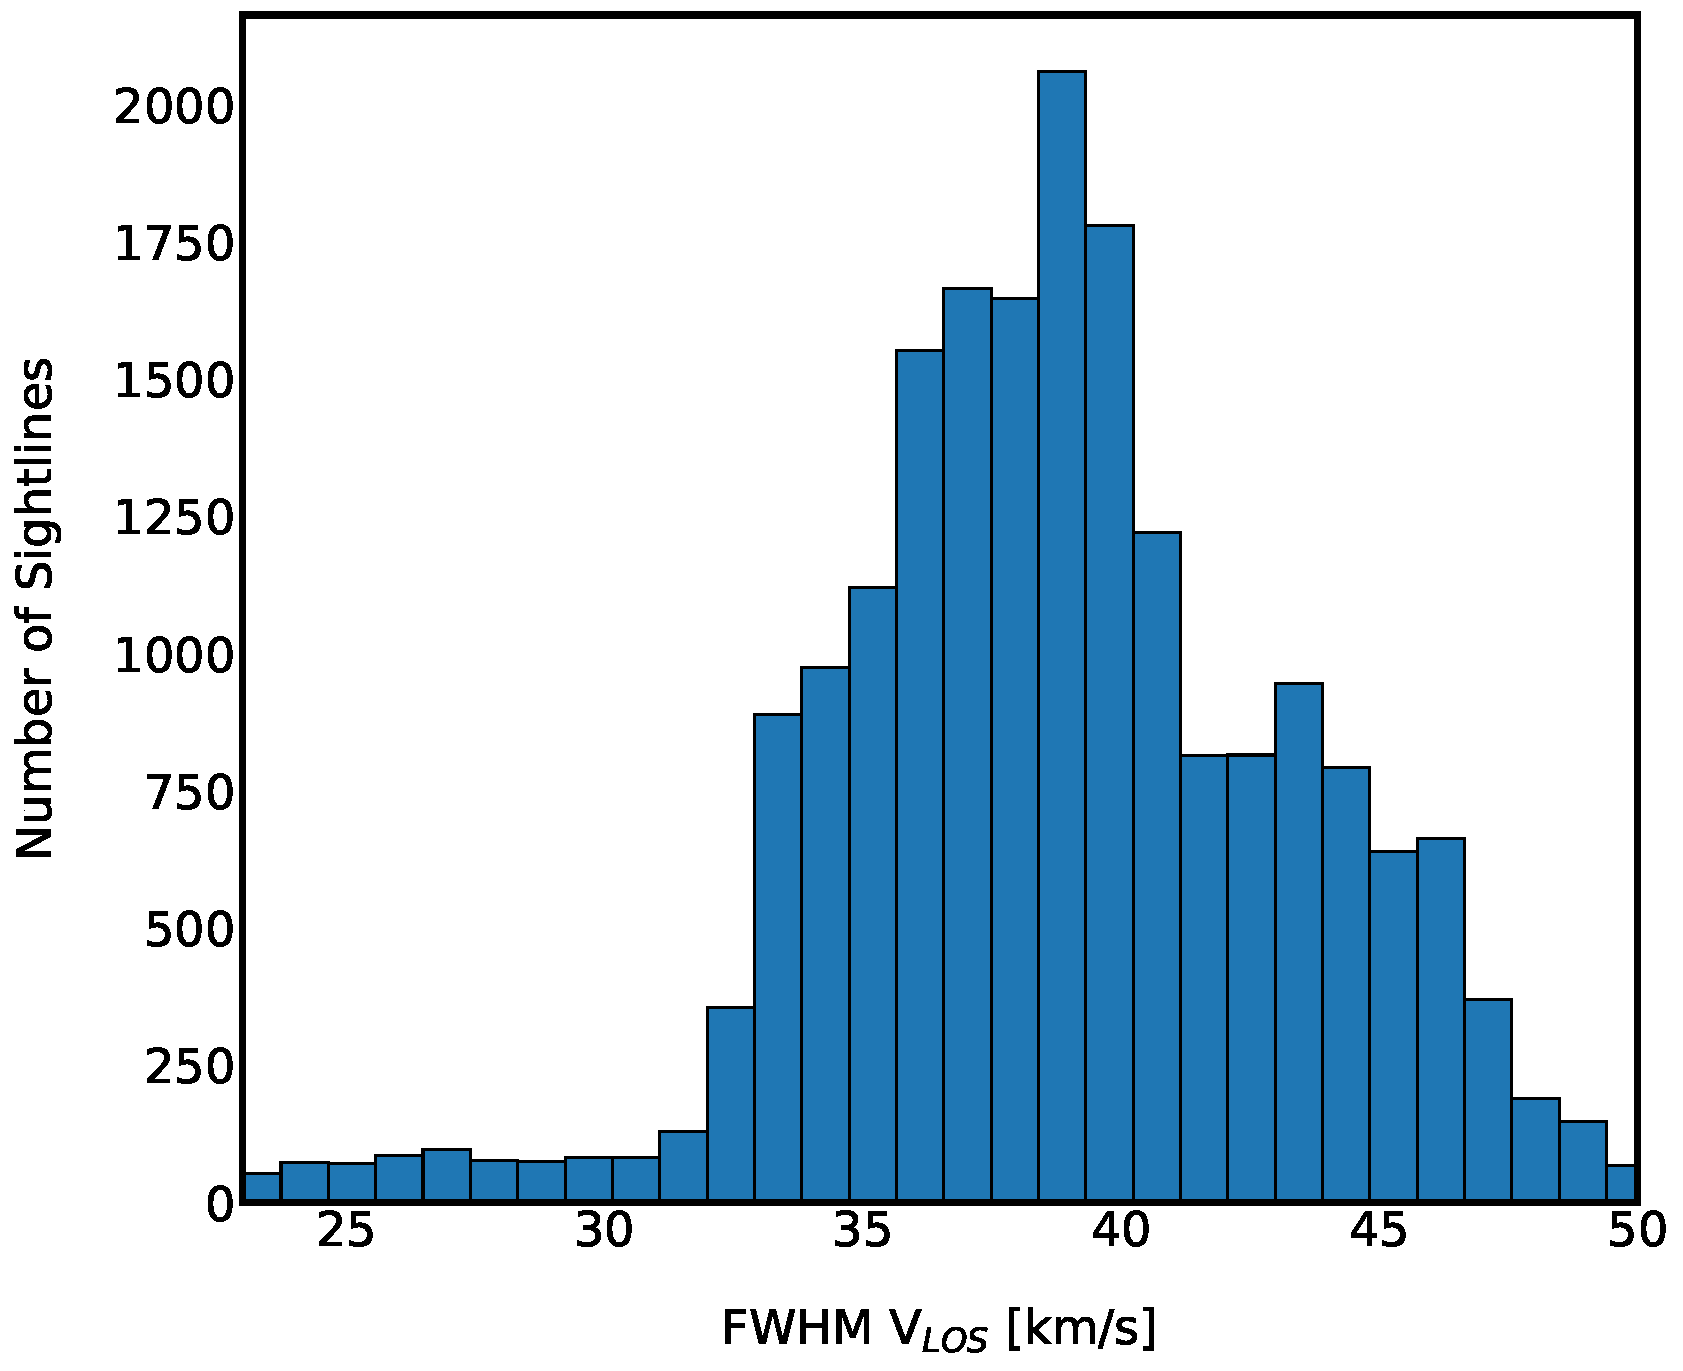
\includegraphics[width=\textwidth]{figures/carina/VLOS_hist}
\caption[A histogram of the FWHM velocity line widths computed over the inner \macrocapwrap{$\sim$1.25~deg$^{2}$} of the BLASTPol CNC map.]{A histogram of the FWHM velocity line widths (in km/s) computed over the inner $\sim$1.25~deg$^{2}$ of the BLASTPol CNC map.}
\label{fig:vfwhm_hist}
\end{figure}

\begin{figure}[!htbp]
\centering
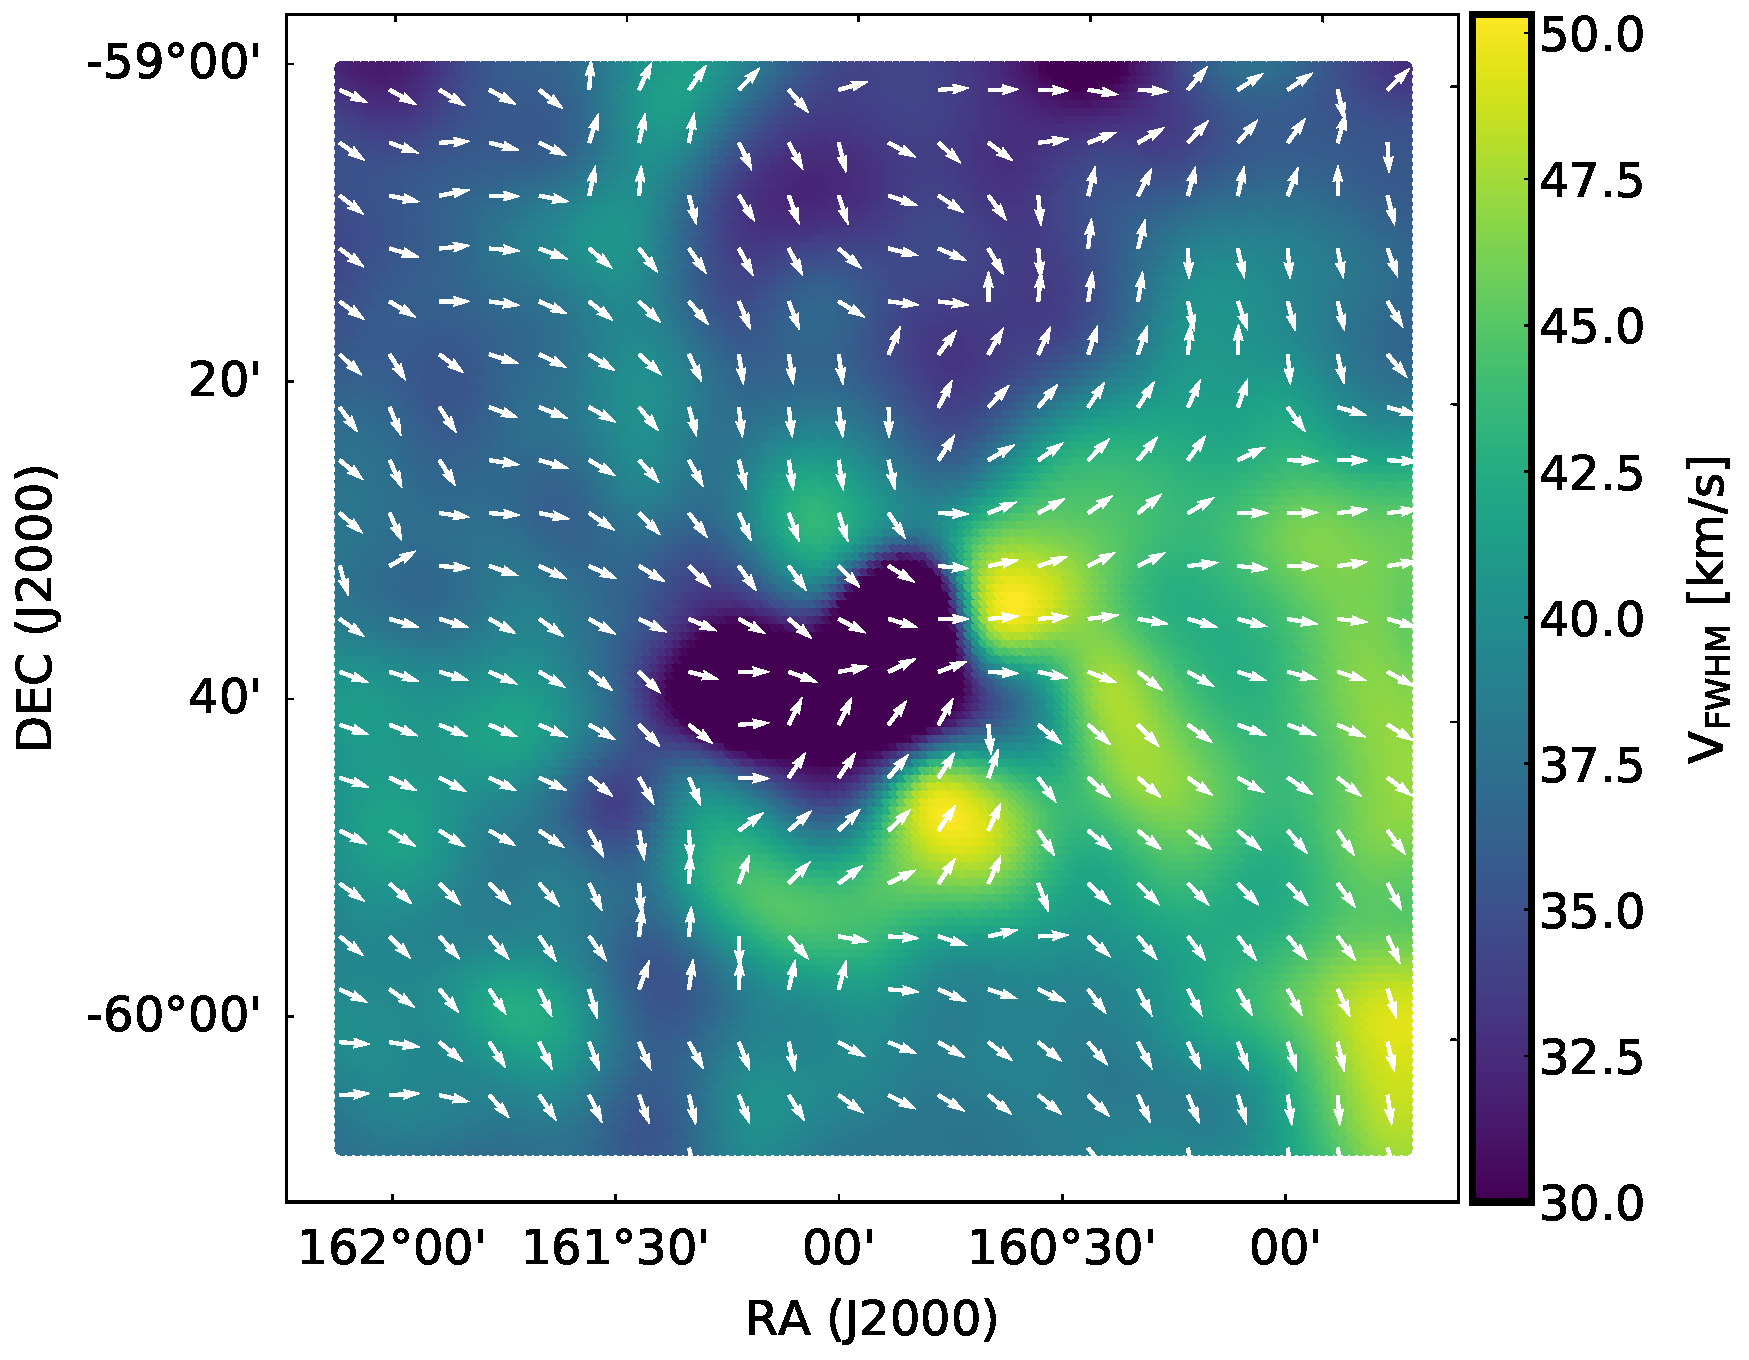
\includegraphics[width=\textwidth]{figures/carina/VFWHM_vectors}
\caption[A map of the FWHM velocity line widths computed from the ATCA HI data cube.]{A map of the FWHM velocity line widths (in km/s) computed from the ATCA $\mathrm{HI}$ data cube. A subset of the \gls{Bpos} pseudovectors (downsampled by 20x) is overplotted in white.}
\label{fig:vfwhm_map}
\end{figure}

\subsection{Uncertainties Associated with the DCFM}\label{DCFM limitations}

For any object, the values of \gls{Bpos} which are produced using Equation~\ref{eq:DCFM 2} carry uncertainties which are important to address. Firstly, the DCFM relies on the assumption that flux-freezing applies in the ROI, and that gravity, turbulence and the B-field together account for the dominant energy densities. For the case of a MC, where the DCFM is typically applied, this assumption may hold true to the extent that any uncertainties it introduces into \gls{Bpos} are sub-dominant to other sources of error. Relative to a single MC, the CNC is complex, containing many $\mathrm{HII}$ regions and powerful sources of energy injection such as the ongoing star formation in Tr~16 and Tr~14. These dynamical processes, along with the aforementioned ones, have conspired together to produce the complex morphology of the CNC that we now observe. Given this disclaimer, the estimates of \gls{Bpos} provided in this work should be taken as preliminary.

The second type of uncertainty carried by the DCFM pertains to $S_{\Phi}$ and $\sigma_{v}$. Because the velocity dispersion is only calculated along the LOS, the method implicitly assumes that the turbulence is isotropic, which is not necessarily the case. Additional uncertainty, represented by the scale factor $Q$ in Equations~\ref{eq:DCFM 1} and~\ref{eq:DCFM 2}, pertain to the relation of the spatial resolution of the polarization and velocity maps to the driving scale of the turbulence in each ROI\@. Several studies have performed MHD simulations of the turbulent environment commonly found in MCs in order to estimate $Q$, and have shown that the B-field estimates produced by the DCFM are sensitive to the level of spatial smoothing which is applied to the maps (see, e.g., \citet{ostriker2001density,padoan2001theoretical,heitsch2001magnetic,kudoh2003nonlinear}).


If \gls{Sphi} is produced by averaging over a region which is larger than the driving scale of turbulence, then \gls{Sphi} will be underestimated, and \gls{Bpos} will be be overestimated (\citet{cho2016technique}). The studies referenced above have shown that $Q$ can range from 0.1--0.7, where the lower limit applies to heavy smoothing, and in the case of a strong B-field with minimal smoothing, $Q$ is usually taken to be 0.5 \citep{houde2004evaluating}. Further uncertainties in \gls{Sphi} and $\sigma_{v}$ are added due to smoothing over inhomogeneities in the gas and dust structures, and confusion between LOS and POS features. In this work, the maps have been smoothed to a physical scale of $\sim$3.5~pc, which is likely to be at least an order of magnitude above the driving scale of turbulence for filaments within the CNC, which are of $\mathcal{O}(0.1)$~pc wide \citep{preibisch2012herschel}. We therefore adopt a conservative value of 0.1 for $Q$, which reduces the $Q$ value of 9.3 in Equation~\ref{eq:DCFM 2} to $Q = 1.86$.

In this work, uncertainty in \gls{nH2} is likely to be the dominant source of error. \gls{NH2}, which is calculated using the Planck \gls{AV} map and canonical relation found in \citet{bohlin224savage}, carries an uncertainty which is sub-dominant to the other measured parameters which factor into the DCFM estimates. However, in order to calculate \gls{nH2}, we have had to assume a column depth for the cloud. The variety of physical configurations present in the ROIs discussed in Section~\ref{multiband comp} require the use of a range of column depths, $L_{\mathrm{CNC}}$. For simplicity's sake, the results shown in the following are produced using $L_{\mathrm{CNC}} = 5$~pc.

\begin{comment}
\begin{equation}
  \frac{\langle B_{t}^{2} \rangle ^{1/2}}{ B_{0} } \simeq \frac{\delta B}{B_{0}} \simeq \frac{\sigma_{v}}{v_{A}}
\end{equation}

\begin{equation}
  \frac{\delta B}{B_{0}} \simeq S_\Phi
\end{equation}
\end{comment}

\subsection{Results of DCFM Applied to the CNC}\label{Bpos estimates}

The \gls{Bpos} maps of the CNC which have been produced using the DCFM include 19,000 sightlines along the inner $\sim$1.25~deg$^{2}$ of the BLASTPol map (they are decimated by a factor of 3 relative to the Stokes maps). Table~\ref{table:dcfm params} lists the estimated values for \gls{Bpos}, v$_{\mathrm{FWHM}}$, \gls{nH2} and \gls{Sphi} for 8 sightlines chosen from the regions defined in Table~\ref{table:regions}. All results presented in this section were produced using the BLASTPol 500~$\upmu$m Stokes maps, and assuming a uniform column depth $L_{\mathrm{CNC}} = 5$~pc.

The results are displayed in several figures included in this section: Figure~\ref{fig:DCFM_5_500} shows the interpolated \gls{Bpos} map with polarization streamlines overplotted in yellow. The ROIs which are defined in Table~\ref{table:regions} are outlined in white, and the reference sightlines from Table~\ref{table:dcfm params} are shown as red dots (the location of $\eta$ Car is shown as a green dot). Figure~\ref{fig:Bpos_LIC} shows the \gls{Bpos}-weighted LIC (LIC$_{500} \times \gls{Bpos}$), with overlays as in Figure~\ref{fig:DCFM_5_500}. Figure~\ref{fig:Bpos_vectors} shows the raw \gls{Bpos} map with a subset of \gls{Bpos} polarization vectors overplotted in white. The Galactic coordinate grid is overplotted in red to illustrate the alignment between \gls{Bpos} and the GP\@. Figure~\ref{fig:Bpos_hist} shows a histogram of \gls{Bpos} over the inner region of the CNC map.

We find that $\langle \gls{Bpos} \rangle = 96$~$\upmu$G and $\sigma_{B} = 100$~$\upmu$G. The maximum value of \gls{Bpos} is 1.2~mG, and the minimum value is close to zero. An idea of the relationship between cloud morphology and \gls{Bpos} can be gleaned from examining Figures~\ref{fig:DCFM_5_500},~\ref{fig:Bpos_LIC} and~\ref{fig:Bpos_vectors}. The highest values of \gls{Bpos} are found in the PDR along the western edge of Tr~14, the lower portion of the NB region (slightly north of Tr~14), around the SP region, and along the eastern edge of the SB\@. There is a concentrated region of high field strength along the southwestern edge of the SB\@. The outlines of several voids other than the SB can clearly be seen in the \gls{Bpos} maps. These are particurly visible in Tr~16, where there is an apparent bubble centered at the approximate location of $\eta$ Car. Others are visible in the NB, and in the region between the SB and SP\@.

Figure~\ref{fig:Bpos_vectors} reveals the extent to which various features within the CNC are aligned with the GP\@. As observed by \citet{li2006results}, the central region of the CNC is in close alignment. The western edge of the SB is largely orthogonal to the GP, as is the region of the SP which contains the highest values of \gls{Bpos}. In Section~\ref{interpreting Bpos}, we discuss these findings in the context of other studies of B-field morphology inside GMCs and HII regions.

\begin{table}[!htbp]
  \centering
\begin{threeparttable}
\begin{tabular}{@{}llllll@{}}
\dtoprule{}
\begin{tabular}[c]{@{}l@{}} RA, DEC \\ (deg J2000) \end{tabular} & \begin{tabular}[c]{@{}l@{}} \gls{Bpos} \\ ($\mathrm{\upmu G}$) \end{tabular} & \begin{tabular}[c]{@{}l@{}} v$_{\mathrm{FWHM}}$ \\ ($\mathrm{km/s}$) \end{tabular} & \begin{tabular}[c]{@{}l@{}} \gls{nH2} \\ ($\mathrm{cm}^{-3}$) \end{tabular} & \begin{tabular}[c]{@{}l@{}} \gls{Sphi} \\ ($\mathrm{deg}$) \end{tabular} & Region \\ \midrule
160.37, -59.78 & 563.85 & 44.68 & 94.59 & 1.43 & 1 \\
160.56, -59.42 & 199.25 & 43.36 & 271.16 & 6.66 & 4 \\
160.61, -60.08 & 487.80 & 38.53 & 37.35 & 0.90 & 1 \\
160.70, -59.59 & 889.48 & 44.74 & 2596.09 & 4.77 & CTR\tnote{1} \\
160.87, -59.75 & 181.29 & 43.66 & 111.54 & 4.73 & 1 \\
160.95, -59.55 & 149.98 & 24.87 & 1550.56 & 12.15 & 2 \\
161.40, -59.73 & 121.11 & 35.87 & 314.25 & 9.77 & 3 \\
161.76, -60.01 & 297.11 & 41.74 & 401.03 & 5.23 & 5 \\ \dbottomrule{}
\end{tabular}
\begin{tablenotes}
\item [1] A sightline near the center of the map.
\vspace{2mm}
\end{tablenotes}
\caption[Physical parameters estimated using the DCFM, for 8 sightlines through the inner region of the CNC.]{Estimates of \gls{Bpos}, $v_{\mathrm{FWHM}}$, \gls{nH2} and \gls{Sphi} for 8 sight-lines along the CNC, produced using the DCFM\@. The regions in column 6 correspond to those in Table~\ref{table:regions}, and are outlined in Figure~\ref{fig:Bpos_LIC}. The sightlines are shown as red dots in Figure~\ref{fig:Bpos_LIC}.}
\label{table:dcfm params}
\end{threeparttable}
\end{table}

% DCFM interp 5~pc 500 um
\begin{figure}[!htbp]
\centering
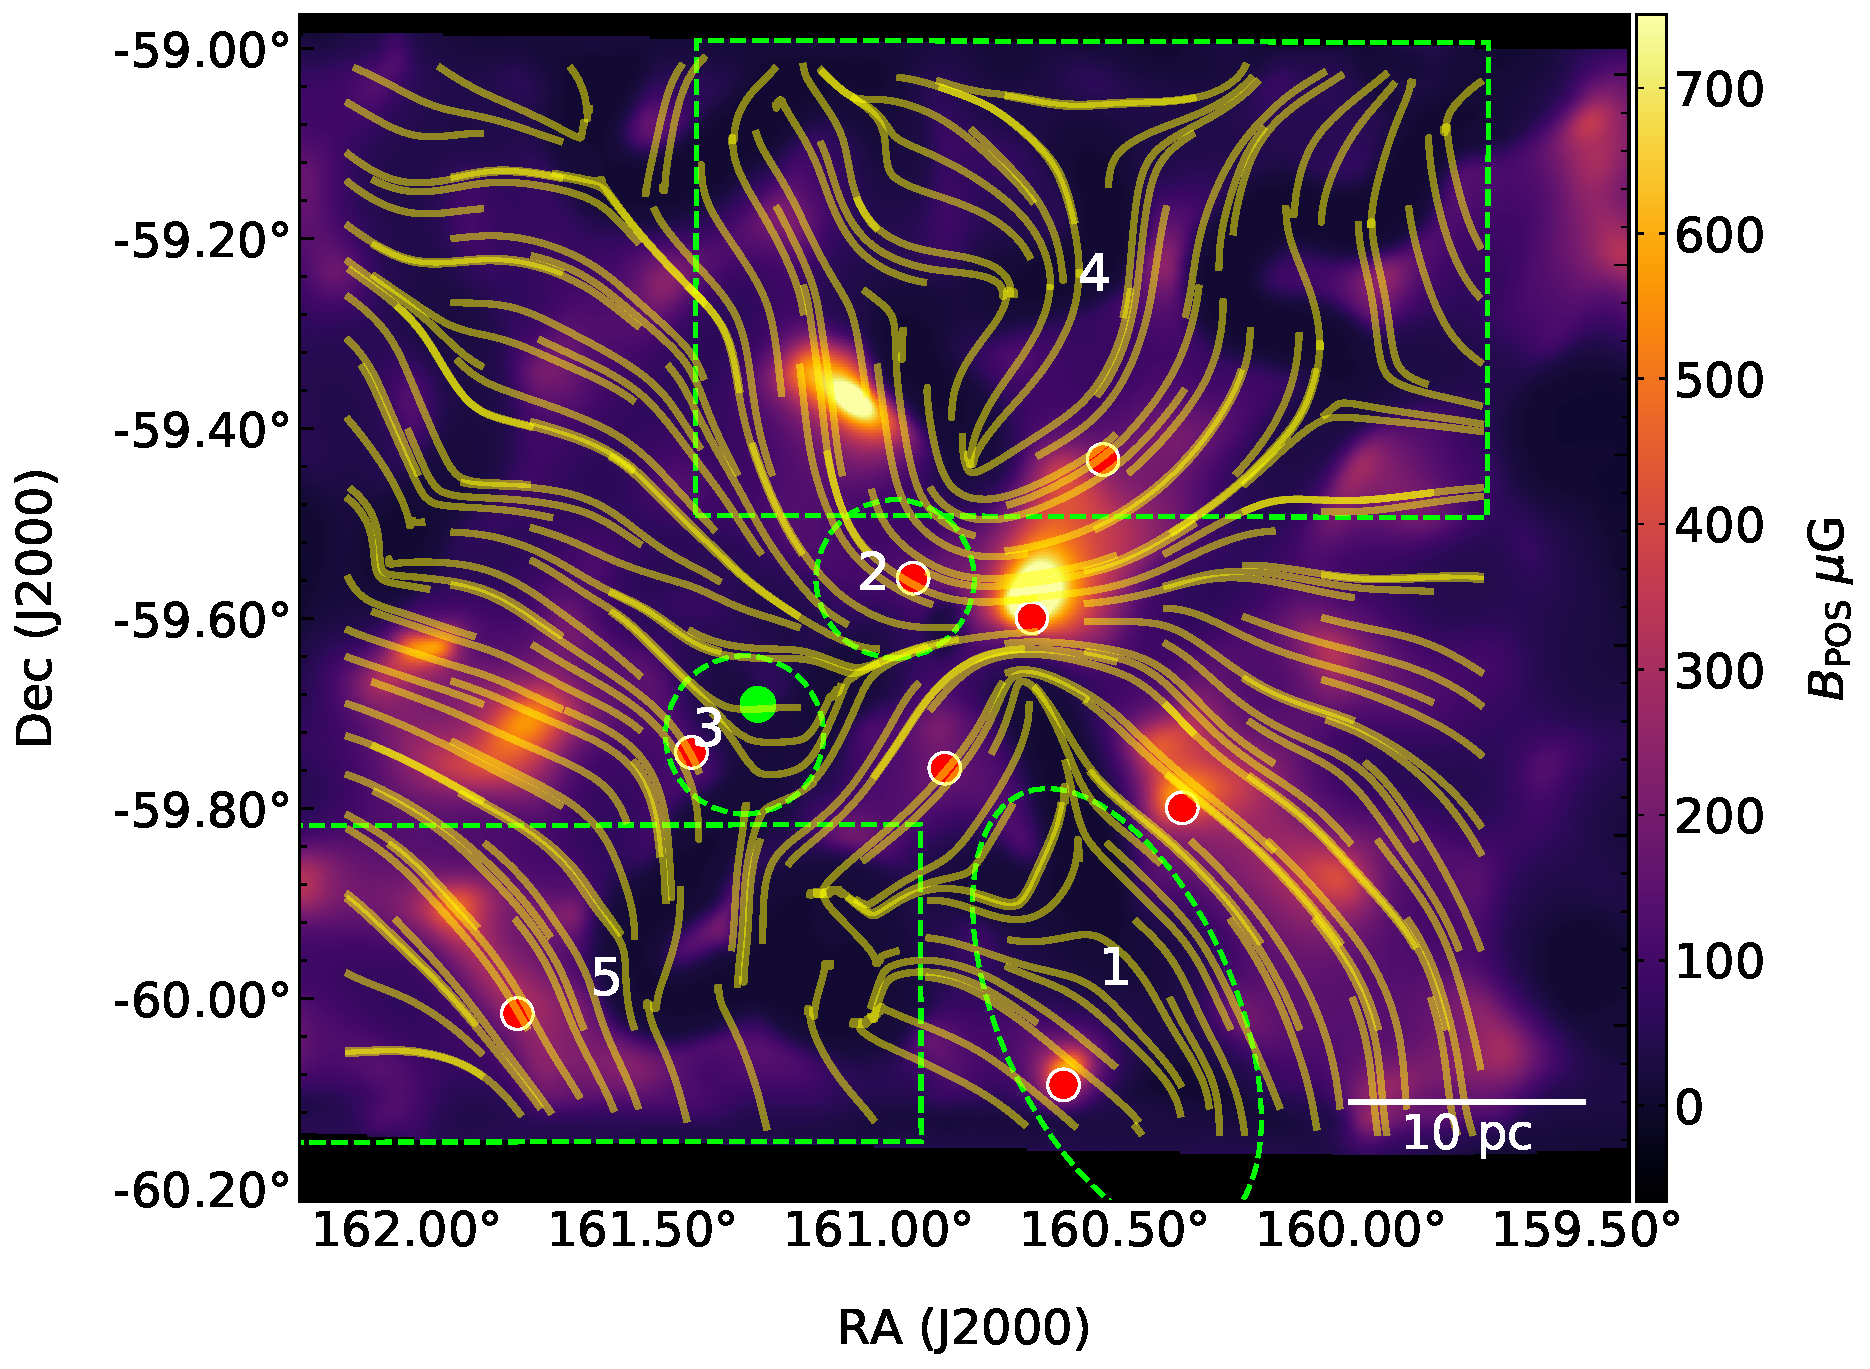
\includegraphics[width=\textwidth]{figures/carina/cftHI_5arcmin_500_5p0pc}
\caption[The \macrocapwrap{\gls{Bpos}$_{,500}$} map (every 3rd pixel interpolated) with polarization streamlines overplotted in yellow.]{The \gls{Bpos}$_{,500}$ map (every 3rd pixel interpolated) with polarization streamlines overplotted in yellow. The outlined ROIs are defined in Table~\ref{table:regions}. Reference sightlines listed in Table~\ref{table:dcfm params} are shown as red dots.}
\label{fig:DCFM_5_500}
\end{figure}

% B vector map 5~pc, 500 um
\begin{figure}[!htbp]
\centering
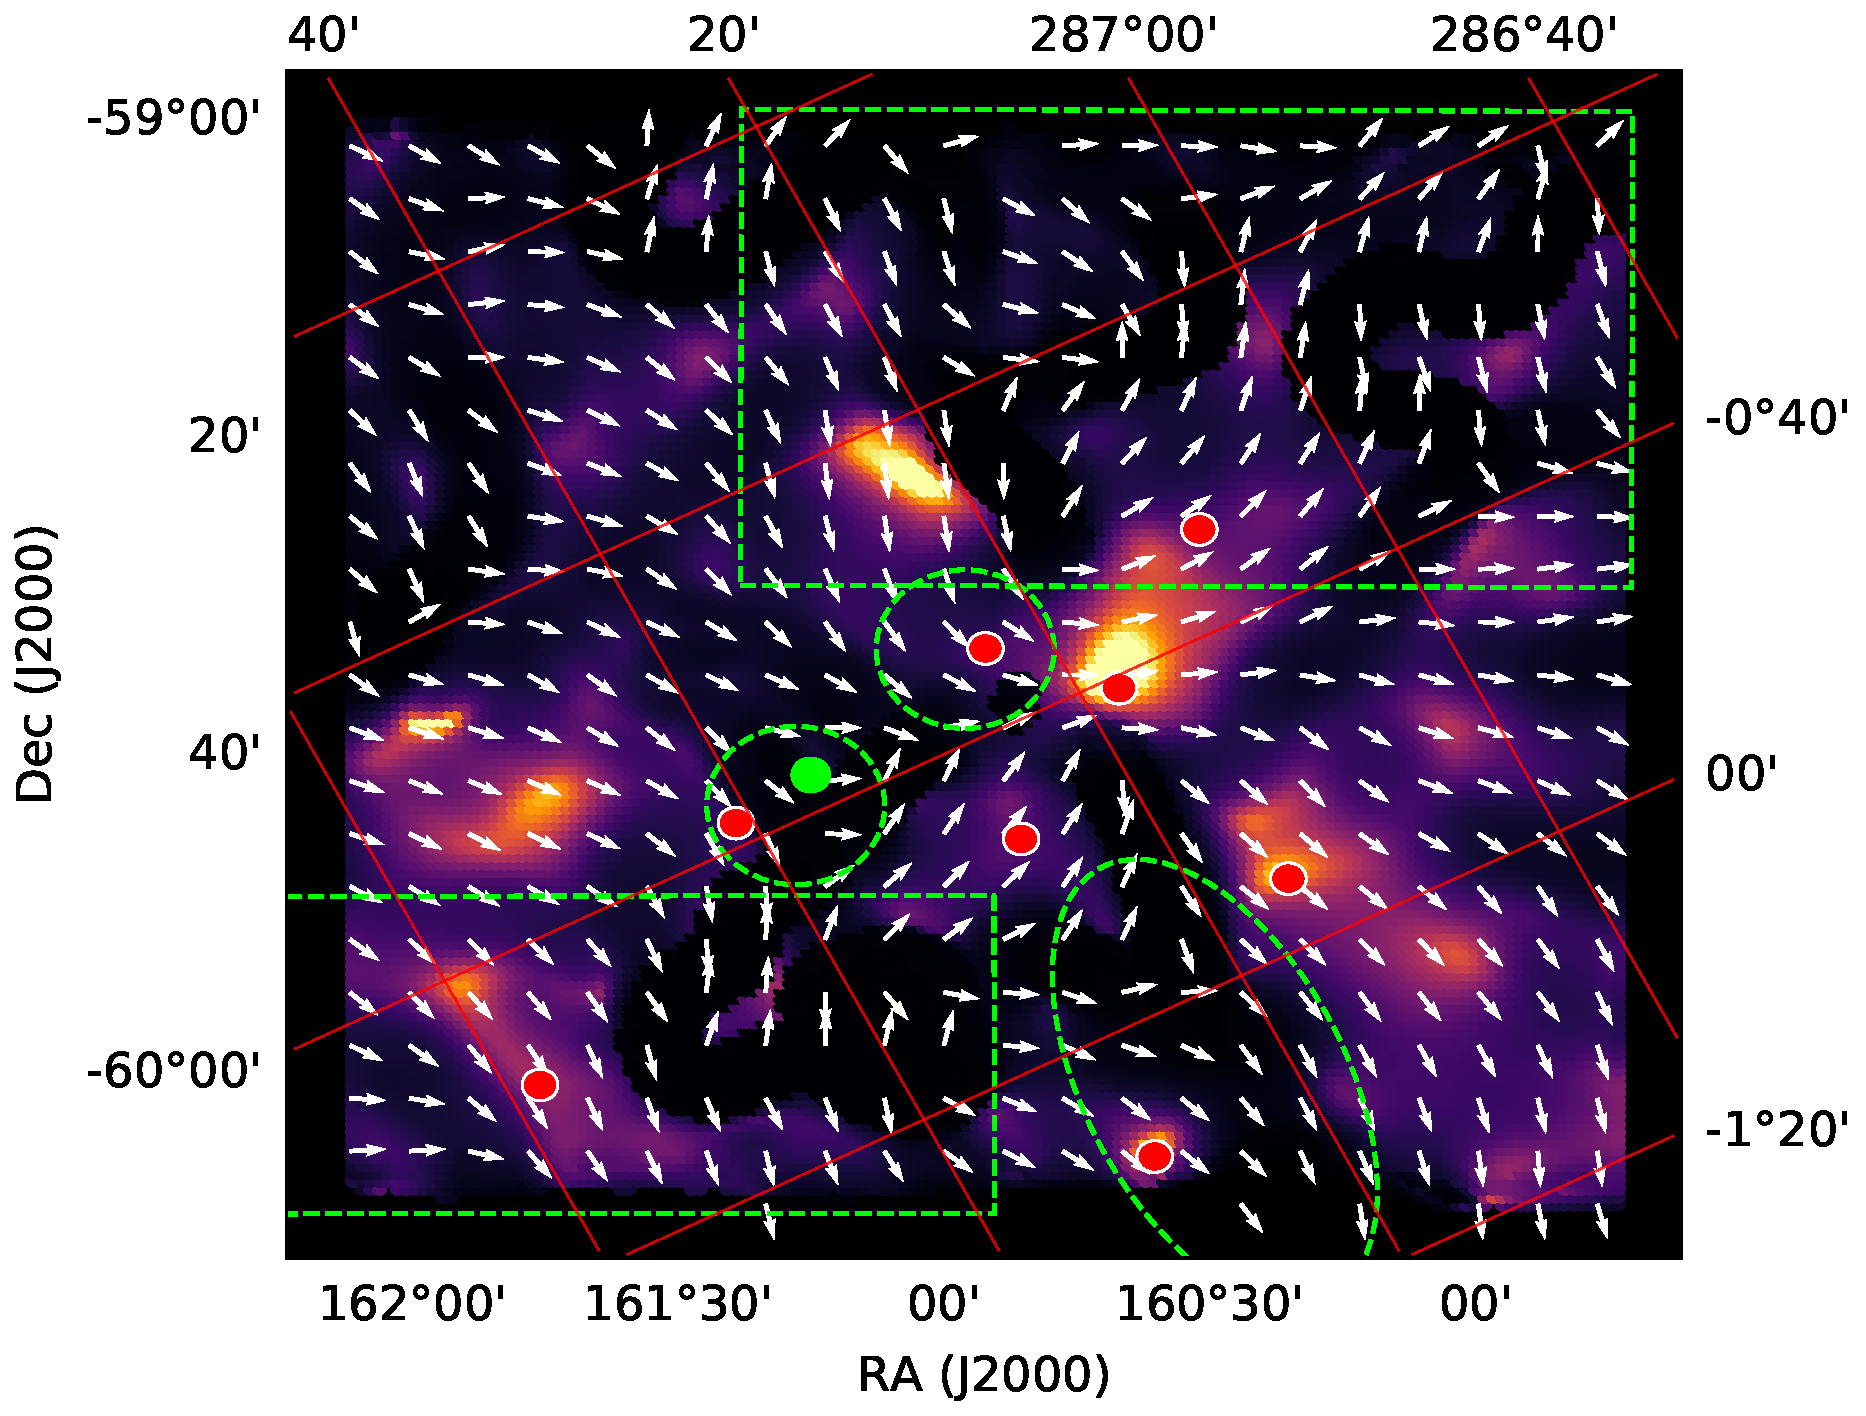
\includegraphics[width=\textwidth]{figures/carina/B_vectors_500_5p0pc}
\caption[The \macrocapwrap{\gls{Bpos}$_{,500}$} map for \macrocapwrap{$L_{\mathrm{CNC}} = 5$}~pc with polarization vectors overplotted in white.]{The \gls{Bpos}$_{,500}$ map for $L_{\mathrm{CNC}} = 5$~pc with polarization vectors overplotted in white. The color scale, in units of~$\upmu$G, is identical to that of Figure~\ref{fig:DCFM_5_500}. Both Galactic and Celestial coordinate frames are labeled, with the Galactic coordinate grid shown in red.}
\label{fig:Bpos_vectors}
\end{figure}

% B LIC 5~pc
\begin{figure}[!htbp]
\centering
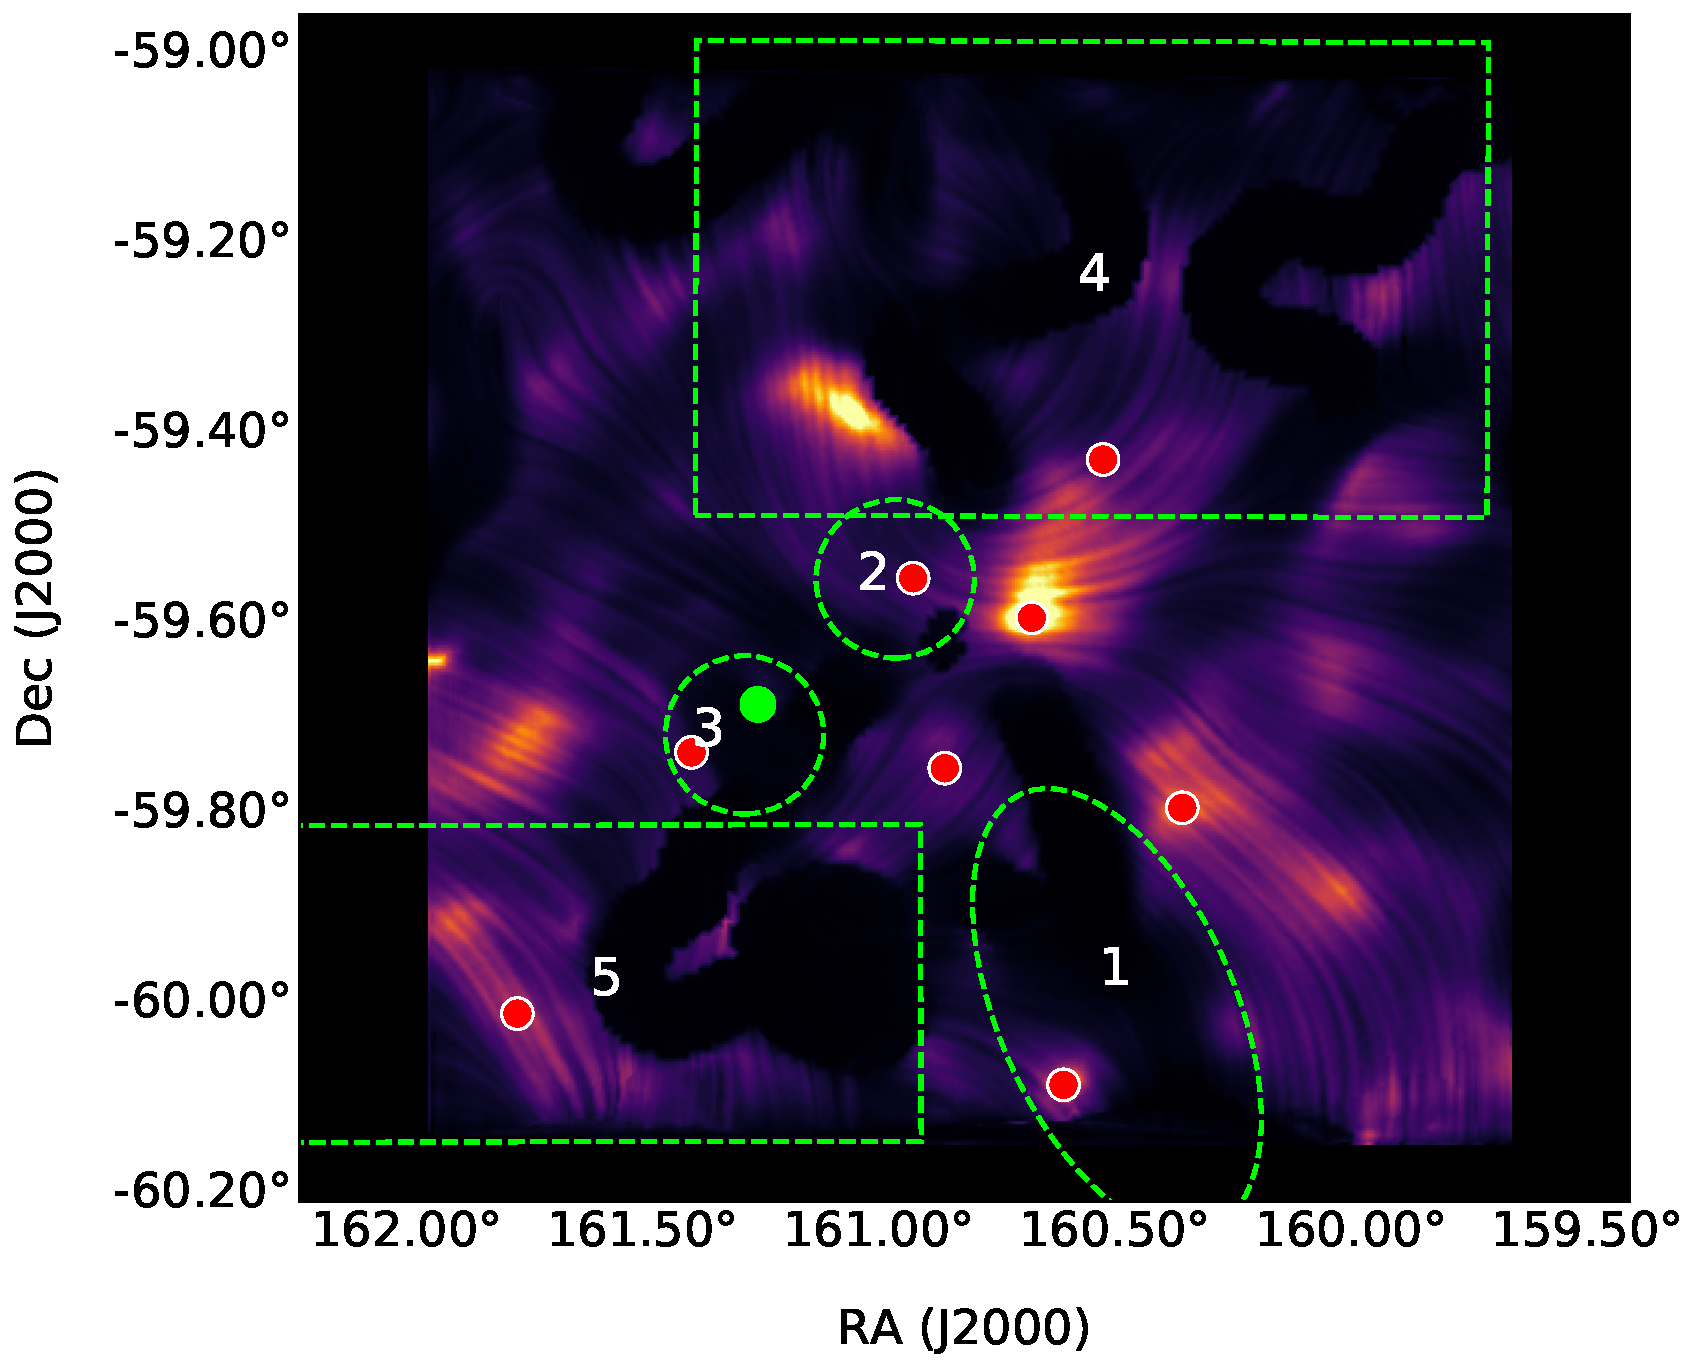
\includegraphics[width=\textwidth]{figures/carina/B_lic_500_5p0pc}
\caption[The \macrocapwrap{\gls{Bpos}} weighted LIC of the \macrocapwrap{500~$\upmu$m} map.]{The \gls{Bpos}-weighted LIC of the 500~$\upmu$m map. The outlined ROIs are defined in Table~\ref{table:regions}. Reference sightlines listed in Table~\ref{table:dcfm params} are shown as red dots.}
\label{fig:Bpos_LIC}
\end{figure}

% B hist 5~pc and 0.5~pc
\begin{figure}[!htbp]
\centering
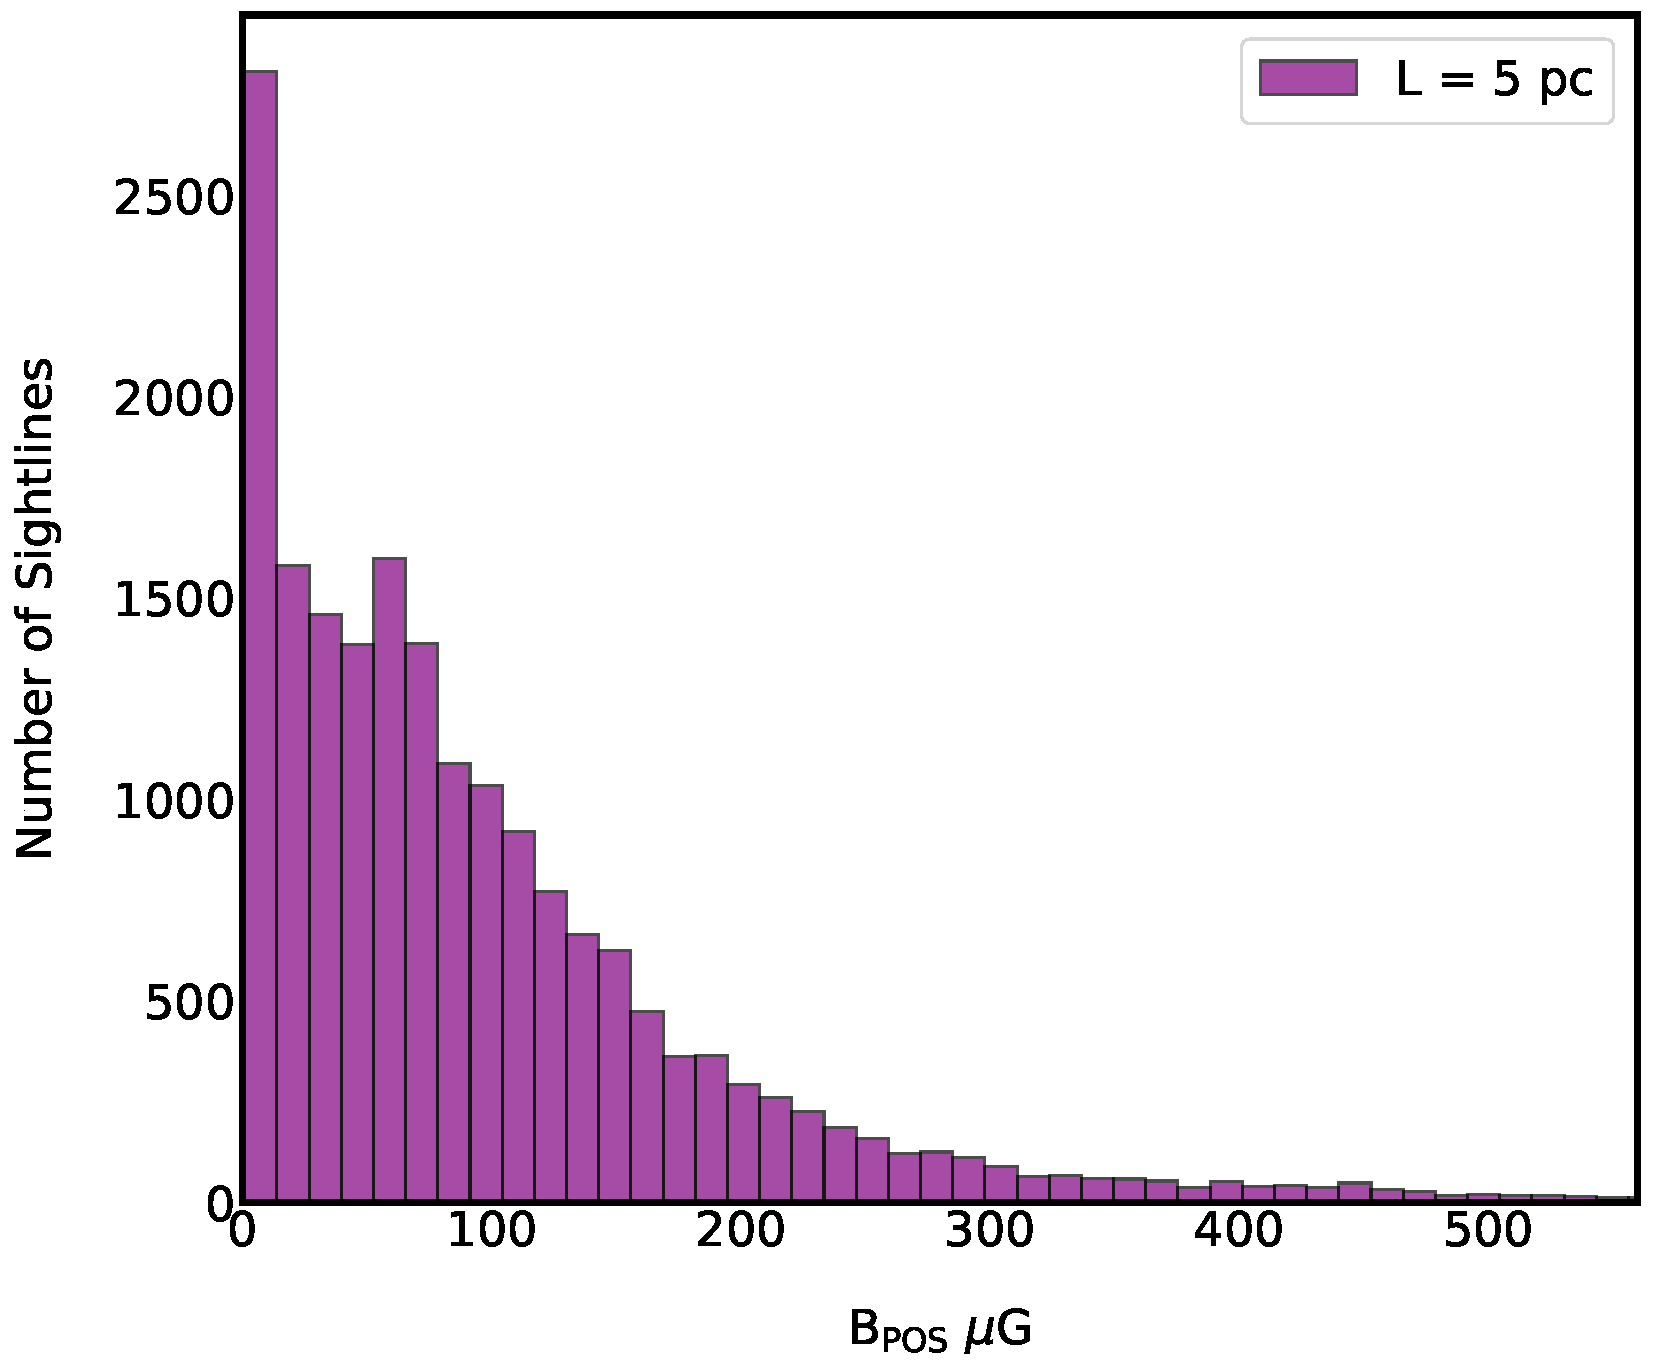
\includegraphics[width=\textwidth]{figures/carina/B_hist_500}
\caption[A histogram of \macrocapwrap{\gls{Bpos}$_{,500}$} over the inner regions of the CNC.]{A histogram of \gls{Bpos}$_{,500}$ within the inner $\sim$1.25~deg$^{2}$ of the BLASTPol CNC field, for an assumed column depth of 5~pc.}
\label{fig:Bpos_hist}
\end{figure}

\subsection{Interpretation of \macrocapwrap{\gls{Bpos}}}\label{interpreting Bpos}

The magnitude of the estimates for \gls{Bpos} in the CNC produced using the DCFM is comparable to estimates which have been made in other GMCs using the same method. \citet{franco2015tracing} applied the DCFM to the Lupus I MC, and found that at large scales \gls{Bpos} is of $\mathcal{O}$(10$^{2}$)~$\upmu$G. In \citet{soler2018magnetic}, the authors applied the DCFM to Planck maps of the Orion-Eridanus superbubble, providing estimates of \gls{Bpos} in the southern edge of the bubble of tens of~$\upmu$G, which were compared to estimates of \gls{Blos} obtained from Zeeman splitting of HI\@. The relationship between \gls{Bpos} and the material at sub-filament scales ($\lesssim$0.1~pc) is of particular interest. MHD simulations of magnetized filaments have predict that there is a critical density, such that \gls{Bpos} is perpendicular to regions of the filament which are above it, and parallel to regions which are below it \citep{soler2013imprint}. The predictions of these simulations have since been verified observationally (see, e.g., \citet{ade2016planck,soler2017relation,fissel2018relative}).

The maps of the CNC used in this analysis do not possess the requisite spatial resolution needed to probe \gls{Bpos} on the scale of sub-parsec filaments (especially after they have been smoothed to the Planck 353~GHz resolution of $\sim$5$\arcsec$). However, their resolution is sufficient enough to allow for an examination of the B-field morphology on the scale of the prominent features listed in Table~\ref{table:regions}.

The question of whether or not B-fields play a significant role in determining the morphologies of Galactic HII regions-- or if the structure of the B-field is shaped by the expanding ionization front, is an active area of research (see, e.g., \citet{churchwell2006bubbling,gendelev2012evolution,anderson2012dust,pavel2012h,tremblin2014age,pellegrini2007magnetically}). As a young HII region expands into the surrounding ISM, the ram pressure of the ionization front encounters resistance from dust and gas which is flux-frozen into the large-scale Galactic B-field. Rather than expand spherically, the shell of the HII region becomes elliptical, with the semi-major axis being parallel to the large-scale direction of the B-field. The B-field then becomes amplified along the long axis of the shell, as parallel lines of flux which are tangential to the expansion direction are forced closer together.

Eventually, the B-field dissipates through magnetic diffusion and mass loading, and the ram pressure of the expanding shell overcomes the resistance from the magnetic pressure \citep{pavel2012h}. If measurements of \gls{Blos} can be obtained via Zeeman splitting or rotation measures, they can be combined with estimates of \gls{Bpos} to formulate a 3D model of the HII region (see, e.g., \citet{aghanim2016planck}). Barring any knowledge of \gls{Blos}, a rough lower limit can be assigned to $B_{\mathrm{\mathrm{tot}}}$ using a simple geometric argument.

Given an HII region with some ellipticity, if all of the ellipticity is assumed to be due to the balance between ram pressure and magnetic pressure, a rough estimate of a lower limit of $B_{\mathrm{\mathrm{tot}}}$ along the edges of the expansion shell. In doing this analysis, bias effects which are due to the inclination angle of the bubble must be considered, as viewing angles which increase the ellipticity of the bubble will produce higher estimates of $B_{\mathrm{\mathrm{tot}}}$. This estimation technique has been applied to ensembles of Galactic HII regions (\citet{churchwell2006bubbling,pavel2012h}). Following \citet{pavel2012h}, we examine the SB region of the CNC (region 1 in Figures~\ref{fig:DCFM_5_500} and~\ref{fig:Bpos_LIC}).

Using Figures~\ref{fig:DCFM_5_500} and~\ref{fig:Bpos_LIC} to roughly estimate the spatial extent of the SB, we assume a shell thickness of $\sim$1~pc. The bubble's fractional thickness $\langle T \rangle$ is calculated as:

\begin{equation}
  \langle T \rangle = \frac{1}{2} \frac{ \sqrt{R_{\mathrm{out}}r_{\mathrm{out}}} - \sqrt{R_{\mathrm{in}}r_{\mathrm{in}}} }{\sqrt{R_{\mathrm{out}}r_{\mathrm{out}}} + \sqrt{R_{\mathrm{in}}r_{\mathrm{in}}}}
\end{equation}

We find $\langle T \rangle = 0.44$, which is comparable to values reported in \citet{pavel2012h} for other HII regions. The fractional thickness is then used to calculate the ratio between the mass density of the shell and mass density of the ISM ($\rho_{\mathrm{shell}}$, $\rho_{\mathrm{ISM}}$) into which it is expanding:

\begin{equation}\label{eq:rho rat}
  \frac{\rho_{\mathrm{shell}}}{\rho_{\mathrm{ISM}}} = \frac{ 1 }{1 - \left( 1 - \langle T \rangle \right)^{3}}
\end{equation}

Using Equation~\ref{eq:rho rat}, we find $\rho_{\mathrm{shell}} = 1.22 \rho_{\mathrm{ISM}}$. For $\rho_{\mathrm{ISM}}$, we assume a value corresponding to $\gls{nH2} \sim 100$, which is roughly the average number density of molecular hydrogen calculated for the region to the west of the shell. The magnitude of $B_{\mathrm{\mathrm{tot}}}$ is estimated by equating the ram pressure of the expanding shell to the magnetic pressure of the large-scale field:

\begin{equation}\label{eq:B_est}
  \begin{aligned}
    P_{\mathrm{ram}} &= P_{B} \\
     \frac{1}{2} \eta \rho_{\mathrm{shell}} u_{s}^{2} &= \frac{B^{2}}{8\pi} \\
  \end{aligned}
\end{equation}

where $u_{s} \approx 10$ km/s is the assumed expansion velocity of the shell, and $\eta = 0.29$ is an efficiency factor calculated in \citet{pavel2012h} which accounts for the inclination angle bias mentioned above. Using Equation~\ref{eq:B_est} to calculate $B_{\mathrm{\mathrm{tot}}}$, we find $B_{\mathrm{\mathrm{tot}}} = 22$~$\upmu$G for $\eta = 1$, and $B_{\mathrm{\mathrm{tot}}} = 12$~$\upmu$G for $\eta = 0.29$. These values are roughly an order of magnitude below the largest values for \gls{Bpos} estimated for the western edge of the shell using the DCFM (first row of Table~\ref{table:dcfm params}). However, they are comparable to the mean value of \gls{Bpos}, $\langle \gls{Bpos} \rangle = 96$~$\upmu$G.

At present, the literature on this subject contains evidence which boths supports and refutes the idea that B-fields may play a significant role in the evolution of HII regions. As noted in \citet{tremblin2014age}, B-fields of $\mathcal{O}$(10$^2$--10$^{3}$) may have sufficient influence over dense gas at small scales, but will likely not influence the morphology of diffuse nebulae on large scales. Additionally, recent MHD simulations of HII region evolution have found that although magnetic pressure may dominate in the atomic gas component of the region, at large scales the radiation pressure plays a more significant role in shaping the bubble \citep{rahner2017winds}. In contrast to the aforementioned findings, in a recent examination of a magnetized PDR in the Galactic HII region M17, \citet{pellegrini2007magnetically} present evidence that the PDR and MC are supported by a B-field with $\langle B \rangle \sim$ 100--600~$\upmu$G (inferred from \gls{Blos} measurements).

These preliminary estimates of \gls{Bpos} in the innermost regions of the CNC are perhaps calculated at too low of a spatial resolution to draw solid conclusions on the significance, if any, which the B-field plays in shaping the various structures within the cloud. Certainly, at large scales, it is likely that they are subdominant to turbulence and ionizing radiation pressure from the many nascent star clusters embedded within the nebula. Future, higher resolution sub-mm observations of the CNC, such as those which are planned to be undertaken by BLAST-TNG in 2019/2020, will hopefully shed more light on the issue.

\begin{comment}
\section{BLAST-TNG Target selection: B-field Morphology in Nearby External Galaxies}

Our understanding of the Milky Way's ISM is greatly augmented by observations of nearby galaxies. Results from the BLAST 2006 balloon flight (2006) revealed that over half of the FIR background originates in galaxies at z $\geq$ 1.2 (\citet{blast2006}). These galaxies are spatially unresolved, although estimates of their global properties may be improved by factoring in inferences made from observations of resolved galaxies. \citet{blastresolved} attempted to constrain estimates of the star formation rate (SFR) in the aforementioned population of unresolved galaxies by placing an upper limit on the amount of AGN (active galactic nuclei) driven dust heating in a sample of six nearby (d $\leq{20}$ Mpc) AGN. This `AGN fraction' is the observed ratio of core flux to extended flux. Using total intensity measurements for six nearby galaxies surveyed by BLAST 2006, the authors were able to derive the dust mass absorption coefficient, and found that the sample of nearby galaxies contains a higher dust mass than would be predicted based on observations of unresolved sub-mm galaxies.

As a sub-mm polarimeter with spatial resolution of $\approx$ 25$\arcsec$ at 250~$\upmu$m, BLAST-TNG will be capable of measuring dozens of \gls{Bpos} pseudovectors for galaxies at distances of around 10~Mpc (a spatial scale of $\sim$1 kpc). This mapping resolution is comparable to that which is commonly achieved by single-dish radio observations at wavelengths of a few centimeters. The resulting maps of \gls{Bpos} can be compared to existing observations of \gls{Bpos} in these targets in order to gain a better understanding of the three-dimensional structure of the large-scale B-field. The total intensity maps will be useful for further analysis of global dust properties within external galaxies. In the following sections, we describe the selection of five nearby galaxies which will be observed during the 2019--2020 BLAST-TNG Antarctic flight. Section~\ref{previous obs} describes some of the key observational inferences about B-fields in external galaxies which have been made to-date. Section~\ref{target selection} summarizes the galaxy targets which have been selected for observation by BLAST-TNG. In Section~\ref{mapping speed} we present estimates of the mapping time required for BLAST-TNG to measure sufficient SNRs on the polarization fraction of each target galaxy.

\section{Summary of Previous Observations}\label{previous obs}

Observations of extragalactic B-fields aim to address the fundamental questions of how the original fields were seeded, amplified, and shaped into their presently observed morphologies. In addition, open questions remain concerning the~degree to which large-scale B-fields influence the evolution of galaxies through the role they play in energetic processes, and in governing the SFR. On galaxy scales, the energy density of B-fields is generally assumed to be in equipartition with that of cosmic rays. In most galaxies, including the Milky Way, the average equipartition B-field strength is of $\mathcal{O}$(10)~$\upmu$G. The field strength is observed to be weaker in radio-quiet galaxies, and stronger in galaxies which host active star formation \citet{beck2016magnetic}. B-fields are physically important on a wide range of scales, from the intergalactic to the interstellar medium (IGM and ISM). They are responsible for channeling cosmic rays throughout (and between) galaxies, and play a role in star formation within MCs. However, astronomical B-fields are difficult to measure. To date, the best tracer of B-fields is polarized emission in wavebands ranging from the radio to the optical. Observations of Zeeman splitting, radio synchrotron emission, Faraday rotation and differential dust extinction (in the optical, NIR or sub-mm/mm-wave bands) can reveal the strength of one or more B-field components. However, Zeeman splitting is the only known measurement technique which can directly probe the strength of the field (for \gls{Blos}).

\subsection{Radio Measurements of External Galaxies}

Over the past few decades, several surveys of polarized synchrotron emission in nearby galaxies have been undertaken in order to map the large-scale fields in a variety of galaxy types, including spirals, ellipticals, dwarf irregulars and interacting pairs \citet{van2015magnetic}. Synchrotron measurements yield estimates of \gls{Bpos}. These measurements can be combined with Faraday rotation measures (RM), which trace \gls{Bpos}, glean information about the three-dimensional structure of the galactic B-fields. The large-scale B-field geometries of a few dozen galaxies have been studied in detail (see, e.g, \citet{sofue1985large},\citet{beck2005magnetic},\citet{beck2016magnetic}). While many of the observed extragalactic B-field configurations can be understood as being the result of small and mean-scale dynamo mechanisms (see Section~\ref{dynamo}), some morphologies defy classification by existing theories (e.g, M81 \citet{beck2006origin}).

These radio observations have led to several key inferences. Perhaps the most wide-reaching inference is the discovery that the integrated radio continuum emission at centimeter wavelengths is strongly correlated (over several orders of magnitude) with the~degree of FIR emission in galaxies with active star formation (the \textit{radio-FIR correlation},  \citet{de1985astronomy}, \citet{beck2008measuring}). Because most of the radio emission at centimeter wavelengths is from non-thermal synchrotron radiation, the synchrotron emission (which traces \gls{Bpos}) can be used to estimate the SFR.

The polarized synchrotron emission, which traces the ordered component of galactic B-fields, has been observed to be strongest in the inter-arm regions of spiral galaxies (\citet{beck2016magnetic}). In these galaxies the toroidal field (field in the plane of the disk) often forms arms which fill the inter-arm regions. These magnetic arms follow the optically bright spiral arms, but occasionally deviate from the large-scale spiral pattern formed by the gas and dust. Within the material arms, the B-field is turbulent and irregular. The poloidal field (the field which occupies the halo), which most easily observed in galaxies with high inclination angles (tending towards edge-on), frequently forms an \textit{X} shape, which is thought to be generated by bipolar outflows of ionized material \citet{ferriere2014analytical}. Figure~\ref{fig:m51} shows a map of \gls{Bpos} pseudovectors in M51, obtained from VLA and Effelsberg measurements at 6 cm, overplotted with an optical image from the Hubble Space Telescope \citet{fletcher2011magnetic}. The inter-arm B-field generally appears to follow the spiral pattern of the optical arms, but extends well beyond the visible extent of the gas and dust.

\begin{figure}[!htbp]
\centering
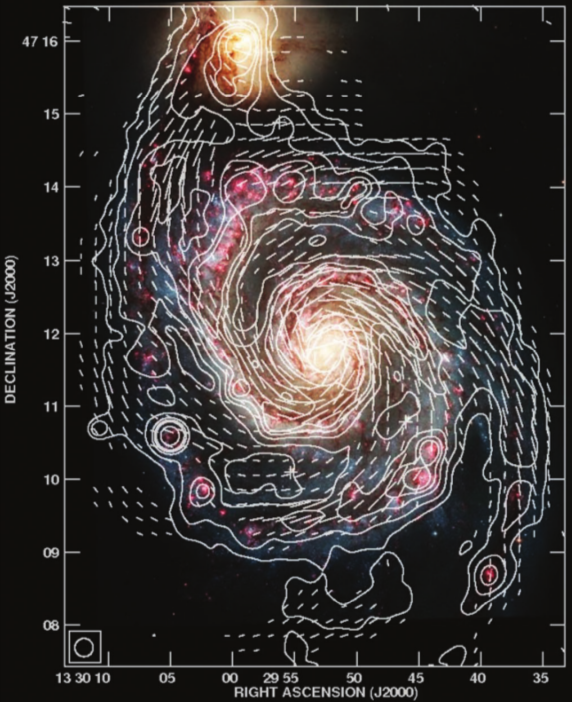
\includegraphics[width=\textwidth]{figures/carina/m51}
\caption[A composite radio image of the large-scale B-field in M51.]{The large-scale B-field in M51 (\gls{Phi} pseudovectors), revealed by VLA and Effelsberg measurements taken at 6 cm, with a spatial resolution of 6$\arcsec$. The background optical image is from the Hubble Space Telescope (\citet{fletcher2011magnetic}.}
\label{fig:m51}
\end{figure}

\subsection{The Modal Structure of Large-Scale Magnetic Fields}\label{dynamo}

Although the mechanism by which the primordial seed fields were created (magnetogensis) is not well understood (see. e.g., \citet{kandus2011primordial}), the theory which describes galactic seed fields are amplified to their observed equipartition values of $\mathcal{O}$(10)~$\upmu$G has for the most part been well matched by observations (\citet{beck2006origin}). The seed fields are thought to have been amplified over several million years by a small-scale dynamo. This dynamo is generated by turbulence created by supernovae and density wave shocks within spiral arms, which shear and compress the B-field. These processes result in a turbulent field geometry, having no regular direction on small scales. The field is then ordered and sustained on large scales over several billion years by the $\alpha-\Omega$ mechanism, where $\alpha$ refers to the Coriolis Effect, and $\Omega$ refers to differential rotation. The mechanism is described by the mean-field dynamo equation:

\begin{equation}\label{eq:dynamo}
\frac{\partial \textbf{B}}{\partial t} = \nabla \times (v \times \textbf{B}) + \nabla \times \alpha \textbf{B} + \eta \nabla^{2} \textbf{B}
\end{equation}

where $\nabla \times (v \times \textbf{B})$ represents field amplification, $\nabla \times \alpha \textbf{B}$ is a gain term from the Coriolis effect, and $\eta \nabla^{2} \textbf{B}$ is a loss term which accounts for the friction of diffusion of ionized and neutral material. For the dynamo to work, gas flows associated with supernova remnants in a disk expand and rise, causing B-field loops to form via the Coriolis effect. In turn, the field loops generate ion flows that produce new, regular fields loops in a plane perpendicular to the disk. The solutions to the mean-field dynamo equation are azimuthal Fourier modes: $\boldsymbol{B} = \sum_{m} \beta_{m}\mathrm{\cos}(m\phi - \beta)$, where $\beta$ is a phase and $\phi$ is the azimuthal angle in the plane of the disk (\citet{sofue1985large}).

The two lowest toroidal modes, axisymmetric (m = 0) and bisymmetric (m = 1), are accompanied by even (quadrupolar) and odd (dipolar) parity poloidal modes. The lower order modes are easier to excitet and amplify than the higher order modes, and most well studied spiral galaxies exhibit a superposition of the two, with axisymmetric being the more dominant mode. Combined radio measurements of polarized synchrotron emission and and Faraday RMs can be used to partially decompose the modes (\citet{beck2008measuring}).

\subsection{Measurements of Polarized Submillimeter Emission in External Galaxies}

Measurements of the sub-mm polarization fraction in external galaxies can advance theories of magnetic dust-grain alignment. They have also been used to characterize the role that external galaxies may play as a CMB foreground (\citet{seiffert2006upper})  In contrast to the growing catalogue of radio observations of external galaxies, there is a paucity of complementary observations of polarized emission at sub-mm wavelengths. Part of this discrepancy is explained by the relatively small number of sub-mm telescopes which possess the spatial resolution of large, single-dish radio observatories. Consequently, more attempts have been made to map \gls{Bpos} on large-scales using differential dust extinction in the optical/NIR (see, e.g., \citet{fendt1998spiral}). Measurements of the sub-mm polarization fraction in external galaxies contributes to

The first sub-mm mapping of \gls{Bpos} in another galaxy was reported for M82, a nearby starbust galaxy \citet{greaves2000magnetic}. This observation was taken at 850~$\upmu$m, with the SCUBA instrument (Submillimeter Common User Bolometer Array) on the James Clerk Maxwell Telescope (JCMT). The spatial resolution of the map is $\sim$15$\arcsec$ ($\sim$280~pc). These observations revealed that M82 possesses a large-scale toroidal field which is ordered on scales of at least that of the map resolution. A poloidal field surrounding the nucleus was also noted. Surprisingly, the orientation of the fields as traced by the polarized sub-mm dust emission were found to be unaligned with the galactic plane.

A more recent sub-mm observation of M82 was taken at 53~$\upmu$m and 154~$\upmu$m with the HAWC+ instrument (High-resolution Airborne Wideband Camera-plus) on the Stratospheric Observatory for Infrared Astronomy (SOFIA). These observations resolved poalrized emission from thermal dust on scales of $\sim$90~pc. A LIC map of \gls{Bpos} at 154~$\upmu$m is shown in Figure~\ref{fig:m82 lic}. The LIC map of M82 shows that \gls{Bpos} has a vertical orientation in the inner region of the galaxy, and a planar orientation in the outer regions of the disk. The inner, vertically oriented field corresponds to the region where a starburst is occurring. The authors of the study note that the high amount of beam-averaging prohibits the application of DCFM to these maps.

\begin{figure}[!htbp]
\centering
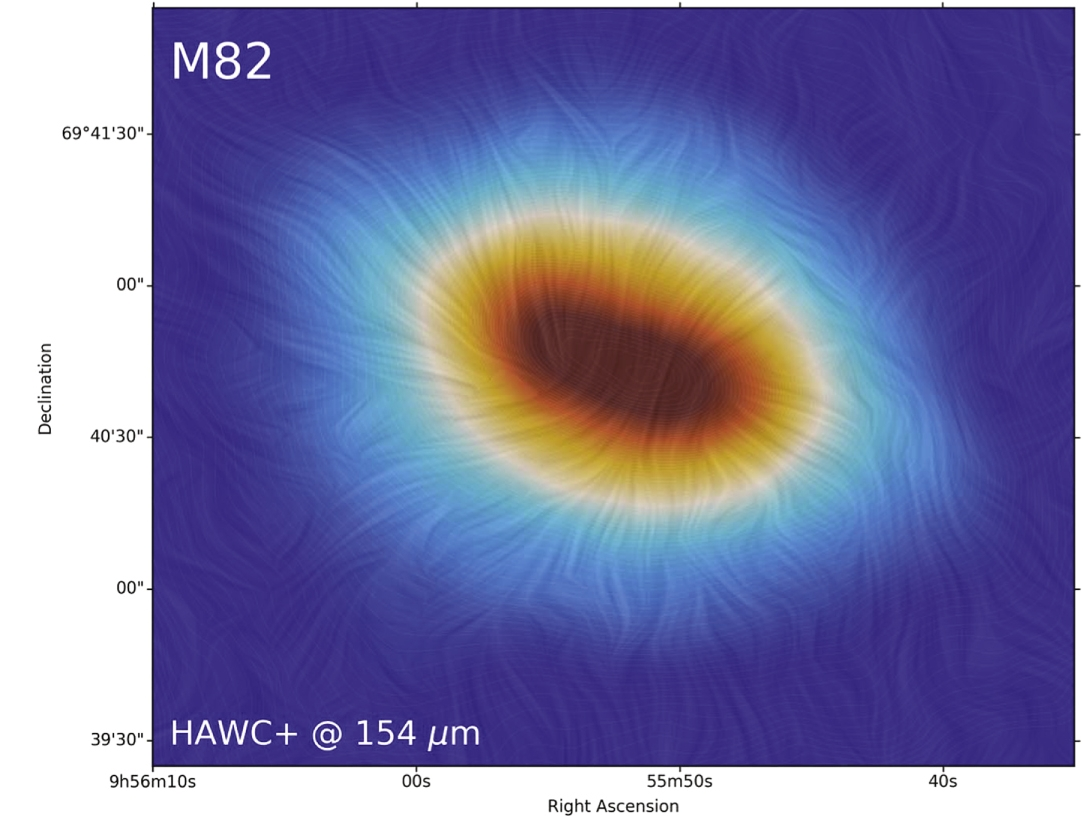
\includegraphics[width=\textwidth]{figures/carina/m82_lic_cropped}
\caption[A LIC map of M82, taken with the \macrocapwrap{154~$\upmu$m} channel of the HAWC+ instrument on SOFIA.]{A LIC map of M82, taken with the 154~$\upmu$m channel of the HAWC+ instrument on SOFIA \citet{jones2019sofia}.}
\label{fig:m82 lic}
\end{figure}

\section{BLAST-TNG External Galaxy Targets}\label{target selection}

The five external galaxies which have been selected for observation by BLAST-TNG were chosen based on several criteria. The primary constraint comes from the telescope's visibility, which will change throughout the flight as the stratospheric circumpolar vortex winds carry the telescope around the Antarctic continent. During the flight, the telescope's latitude might change by up to 10~degrees. The telescope can move in elevation between 22 and 50~degrees, with limits on azimuth imposed by the position of the sun (it should be kept out of view of the primary mirror). Roughly, observable targets must fall within the range of 5 to 18 hours of RA, and -62 to -23~degrees of declination.

The second selection criterion is that the galaxies be bright enough for BLAST-TNG to be able to measure an SNR on the polarization fraction of $\gtrsim$ 3 (see Section~\ref{mapping speed}). Lastly, galaxies that satisfy the first two criteria are deemed more desirable if previous observations of their B-fields exist, particularly those based on measurements of polarized synchrotron emission or Faraday RMs.

\subsection{Target List}\label{targ list}

The five galaxy targets, along with their sky coordinates, distance, resolvable spatial scale at 250~$\upmu$m and type are listed in Table~\ref{table:gal targs}.

%\begin{threeparttable}[!htbp]
\begin{table}[!htbp]
\centering
\begin{tabular}{@{}llllll@{}}
\dtoprule
Object & RA (J2000) & DEC (J2000) & \begin{tabular}[c]{@{}l@{}} Distance \\ (kpc) \end{tabular} & \begin{tabular}[c]{@{}l@{}}Scale$_{250}$ \\ (kpc) \end{tabular} & Type  \\ \midrule
NGC 4945 & 13:05:27.279 & -49:28:04.44 & 3,900 & 0.57 & SB(s)cd \\
ESO 97-G13 & 14:13:09.906 & -65:20:20.47 & 4,200 & 0.61 & SA(s)b \\
% NGC 5068 & 13:18:54.807 & -21:02:20.76 & 6,075 & 0.82 & SB(s)d \\
NGC 3621 & 11:18:16.5     & -32:48:51  &  6,700 & 0.97 & SA(s)d \\
NGC M83 & 13:37:00.919 & -29:51:56.74 & 8,900 & 1.29 & SA(s)ab \\
NGC 1808 & 05:07:42.343 & -37:30:46.98 & 10,900 & 1.59 & (R$^{\prime}$)SAB(s)b \\
% NGC 2997 & 09:45:38.793 & -31:11:27.92 & 15,900 & 2.31 & SA(s)c\\ \bottomrule
\\
\end{tabular}
%\begin{tablenotes}
%    \item[1] Laboca.\\
%  \end{tablenotes}
\caption{A summary of the five nearby galaxy targets selected for observation by BLAST-TNG, listed in order of their distance.}
\label{table:gal targs}
\end{table}

\textit{NGC 4945}: NGC 4945 is an edge-on, Seyfert 2 (Sy2) type spiral galaxy which is otherwise thought to be similar to the Milky Way (\citet{spoon2000mid}). To date, no radio halo has been detected in NGC 4945 (\citet{elmouttie1997radio}).

\vspace{5mm}

\textit{ESO 97-G13}: ESO 97-G13 (AKA the \textit{Circinus Galaxy}) is a near edge-on Sy2 galaxy located close to the Galactic plane. Its bipolar radio lobes have been mapped at centimeter wavelengths with ATCA (\citet{elmouttie1998radio}). The radio lobes are associated with ionized plumes being ejected from the active galactic nucleus. The B-field in the radio lobes is observed to be aligned with the plume axis.

\vspace{5mm}

\textit{NGC 3621}: NGC 3621 is a near edge-on spiral field galaxy. There is no evidence for a bulge in the galaxy's center, but it is thought to be a Sy2 type (\citet{barth2008dynamical}). The HI continuum was recently mapped at 6$\arcsec$ resolution with the Very Large Array (VLA), as part of the THINGS survey of nearby galaxies (\citet{walter2008things}).

\vspace{5mm}

\textit{M83}: M83 (NGC 5236, AKA the \textit{Southern Pinwheel Galaxy}) is a nearby, nearly face-on grand-design spiral galaxy of the starburst variety. It is located near the dwarf galaxy, NGC 5253, which also hosts a high level of active star formation. M83 has been observed in a wide range of wavebands, and the large-scale structure of its B-field has been mapped in polarized synchrotron emission (\citet{sukumar1989large}, \citet{frick2016magnetic}). The B-field is of the inter-arm spiral type. The authors of \citet{frick2016magnetic} compared the radio observations of M83 to sub-mm total intensity maps, and found that the orientation of one of the main B-field arms is misaligned with its corresponding gaseous arms.

%\textit{NGC 2997}: NGC 2997 is a face-on unbarred spiral galaxy, whose scale B-field has previously been mapped using Faraday RMs (\citet{han1999magnetic}). The RM map revealed an anomalous field reversal between the disk and central region of the galaxy. An unusually high~degree of radio polarization  ($\sim$25\%) has been reported along the inner edges of the galaxy's spiral arms (\citet{beck2016magnetic}).

\vspace{5mm}

\textit{NGC 1808}: NGC 1808 is an Sy2 type galaxy which was observed by BLAST 2006 in 250, 350 and 500~$\upmu$m total intensity (\citet{blastresolved}). Its large-scale B-field has been mapped in optical polarization, which revealed a coherent toroidal magnetic spiral, with no visible poloidal component. \citet{siebenmorgen2001infrared} detected polarized emission at 170~$\upmu$m along four sightlines through the galaxy, and found that the polarization angles differ significantly from those measured from non-thermal polarized radio emission (\citet{siebenmorgen2001infrared}).

%\vspace{5mm}

%\textit{NGC 5068}: NGC 5068 is a nearly face-on, barred spiral galaxy. It has been found to be radio-weak, with no halo polarization detected to date (\citet{beck2005magnetic}).

%IRAS
%\citet{neugebauer1984infrared}
%PHANGS
%\citet{leroy2016portrait}
%KINGFISH
%\citet{dale2012herschel}

\subsection{Required Observing Times}\label{mapping speed}

In this section we present estimates of the minimum integration times which are required to make 3-$\sigma$ measurements of the polarization fraction $p$ for each of the galaxy targets described in Section~\ref{targ list}. A detailed description of the methods presented here can be found at \url{https://sites.northwestern.edu/blast/}.

The minimum beam-averaged source intensity (MJy/sr) which is required to achieve 1-$\sigma$ error bars on the polarization fraction of $\sigma_{p}$, over a map of area $A_{map}$ (deg$^{2}$), in $t$ hours, is:

\begin{equation}\label{eq:Ireq}
  I_{req} = I_{ref} \left( \frac{A_{map}}{1 \text{~deg}^{2}}  \right)^{1/2} \left( \frac{5 \text{ hr}}{t} \right)^{1/2} \left( \frac{0.005}{\sigma_{p} } \right) \qquad \left[ \text{MJy/sr} \right]
\end{equation}

where $I_{ref}$ (MJy/sr) is the beam-averaged source intensity which is required to measure $\sigma_{p}$ = 0.5\%, after 5 hr integration over a 1~deg$^{2}$ map (see Table~\ref{table:map speed}). The required observing time to achieve 1-$\sigma$ error bars on $p$ of $\sigma_{p}$ over a map of area $A_{map}$ (deg$^{2}$), for a source with beam-averaged intensity $I_{req}$, is:

\begin{equation}\label{eq:treq}
  t_{req} = t_{ref} \left( \frac{A_{map}}{1 \text{~deg}^{2}}  \right) \left( \frac{0.005}{\sigma_{p} } \right)^{2} \left(  \frac{100 \text{ MJy/sr}}{I_{req}} \right)^{2} \qquad \left[ \text{hr} \right]
\end{equation}

where $t_{ref}$ is the time required to obtain $\sigma_{p} = 0.5$\% for a source with $I = 100$ MJy/sr (see Table~\ref{table:map speed}).

\begin{table}[!htbp]
\centering
\begin{tabular}{@{}llll@{}}
\dtoprule
 & 250~$\upmu$m & 350~$\upmu$m & 500~$\upmu$m \\ \midrule
$I_{ref}$ (MJy/sr) & 188.7 & 113.7 & 42.4 \\
$t_{ref}$ (hr) & 17.8 & 6.4 & 0.9 \\
Beam FWHM ($\arcsec$) & 30 & 41 & 59 \\ \bottomrule
\\
\end{tabular}
\caption[Reference values for calculating the required target intensity \macrocapwrap{$I_{req}$} and observation time \macrocapwrap{$t_{req}$} to achieve a desired maximum uncertainty on the polarization fraction \macrocapwrap{$\sigma_{p}$}.]{Reference values for calculating the required target intensity $I_{req}$ and observation time $t_{req}$ to achieve a desired maximum uncertainty on the polarization fraction $\sigma_{p}$. The reference intensity $I_{ref}$ (MJy/sr) is the beam-averaged source intensity which is required to measure $\sigma_{p}$ = 0.5\%, after a 5 hr integration over a 1~deg$^{2}$ map. The reference integration time $t_{ref}$ (hr) is the time required to obtain $\sigma_{p} = 0.5$\% for a source with a beam-averaged intensity of 100 MJy/sr. Table values are taken from \url{https://sites.northwestern.edu/blast/}. The beam FWHM for each observation band (in arcsec) is listed in the third row.}
\label{table:map speed}
\end{table}

The smallest maps that BLAST-TNG will make will be $\sim$0.5~deg$^{2}$. Because the galaxy targets fit into this area, their map size will be uniformly $\sim$0.5~deg$^{2}$. Table~\ref{table:treq} lists the required integration time $t_{req}$, in hours, needed to achieve $\sigma_{p} = 0.5$\% over the region of each galaxy which is visible in the the Herschel 250~$\upmu$m total intensity maps. Three of the targets require at least 7 hours of integration time. The brightest targets, NGC 4945 and ESO 97-G13, require at least 3 hours.

\begin{table}[!htbp]
\centering
\begin{tabular}{@{}lllll@{}}
\dtoprule
Object & A$_{map}$ (deg$^{2}$) & $\sigma_{p}$ (\%) & t$_{req}$ (hr) & I$_{250}$ center (MJy/sr) \\ \midrule
NGC 4945 & 0.5 & 0.5 & 3 & 10,000 \\
ESO 97-G13 & 0.5 & 0.5 & 3 & 3,600 \\
NGC 3621 & 0.5 & 0.5 & 7 & 150 \\
M83 & 0.5 & 0.5 & 7 & 1,000 \\
NGC 1808 & 0.5 & 0.5 & 7 & 2,500 \\ \bottomrule
\\
\end{tabular}
\caption[Key mapping parameters for the BLAST-TNG external galaxy targets.]{Map area $A_{map}$, 1-$\sigma$ polarization fraction $\sigma_{p}$, integration time $t_{req}$, and central beam-averaged intensity from Herschel 250~$\upmu$m maps for each BLAST-TNG galaxy target}
\label{table:treq}
\end{table}

Figures~\ref{fig:ngc4945} to~\ref{fig:ngc1808} show the Herschel 250~$\upmu$m maps for each galaxy target. The color scales are (left frame) $t_{req}$ in hours, and (right frame) beam-averaged intensity in MJy/sr.

\begin{figure}[!htbp]
\centering
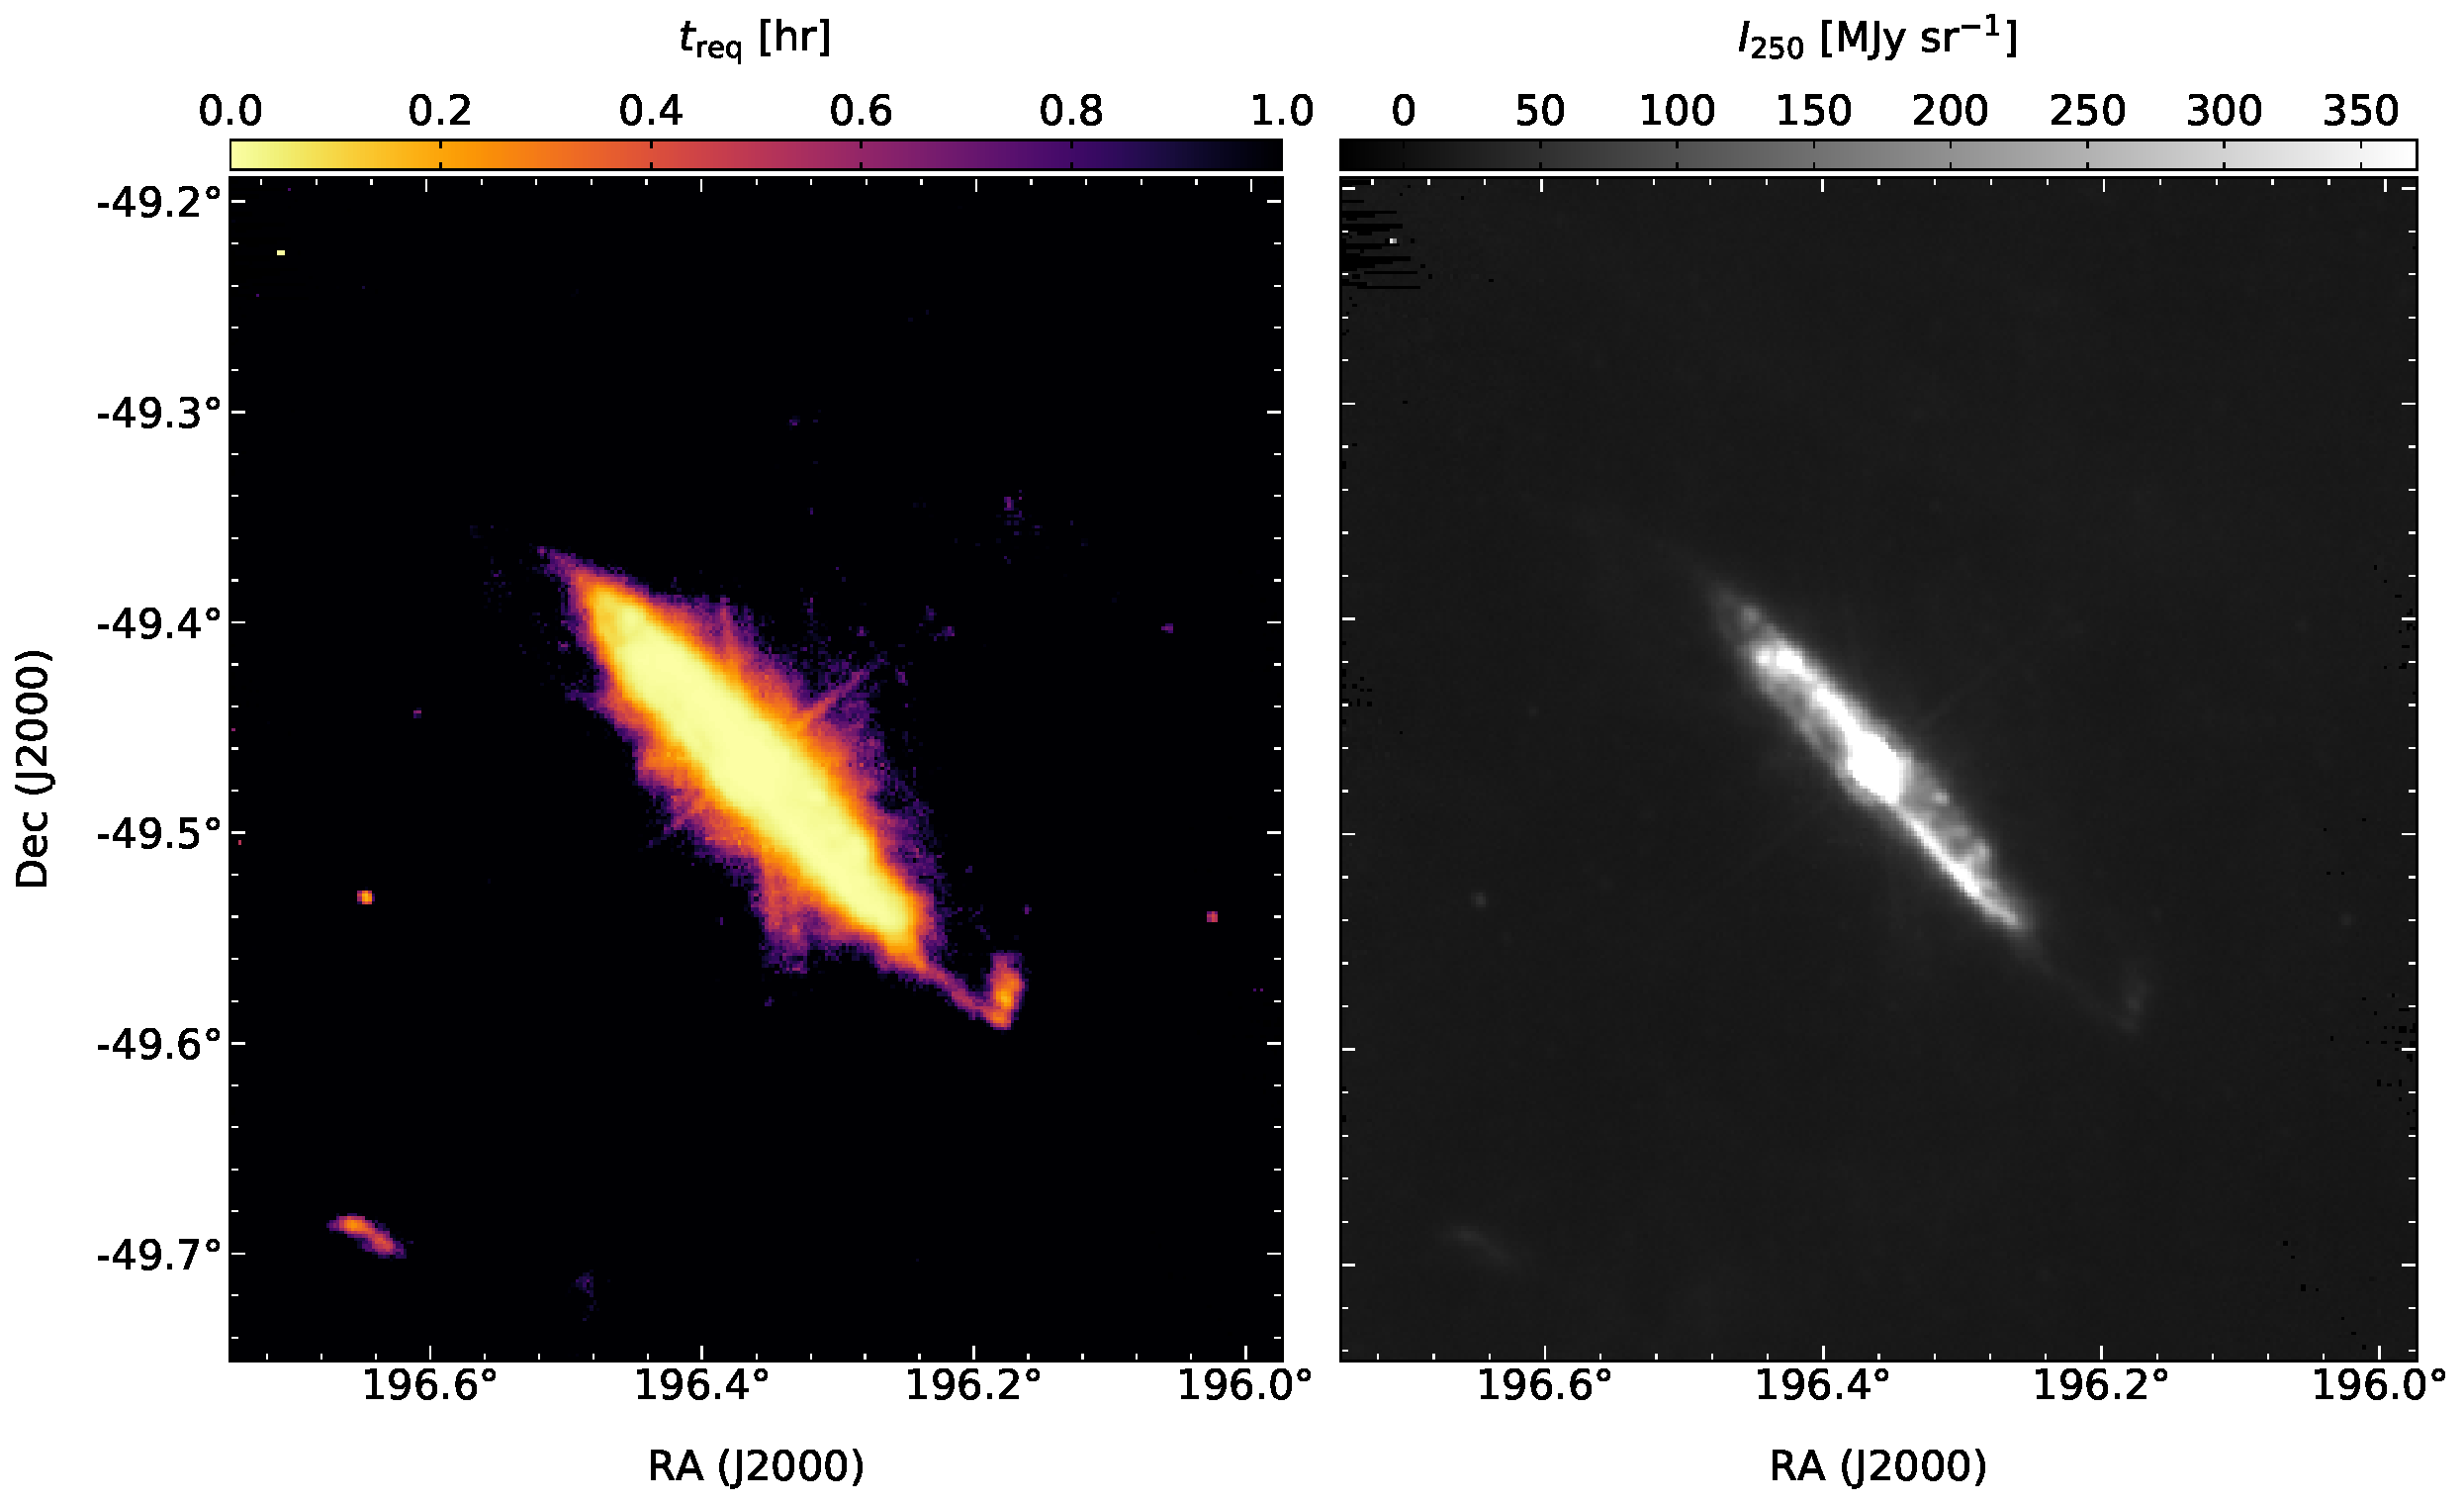
\includegraphics[scale=0.35]{figures/carina/ngc4945}
\caption[NGC 4945.]{NGC 4945, images from Herschel 250~$\upmu$m.}
\label{fig:ngc4945}
\end{figure}

\begin{figure}[!htbp]
\centering
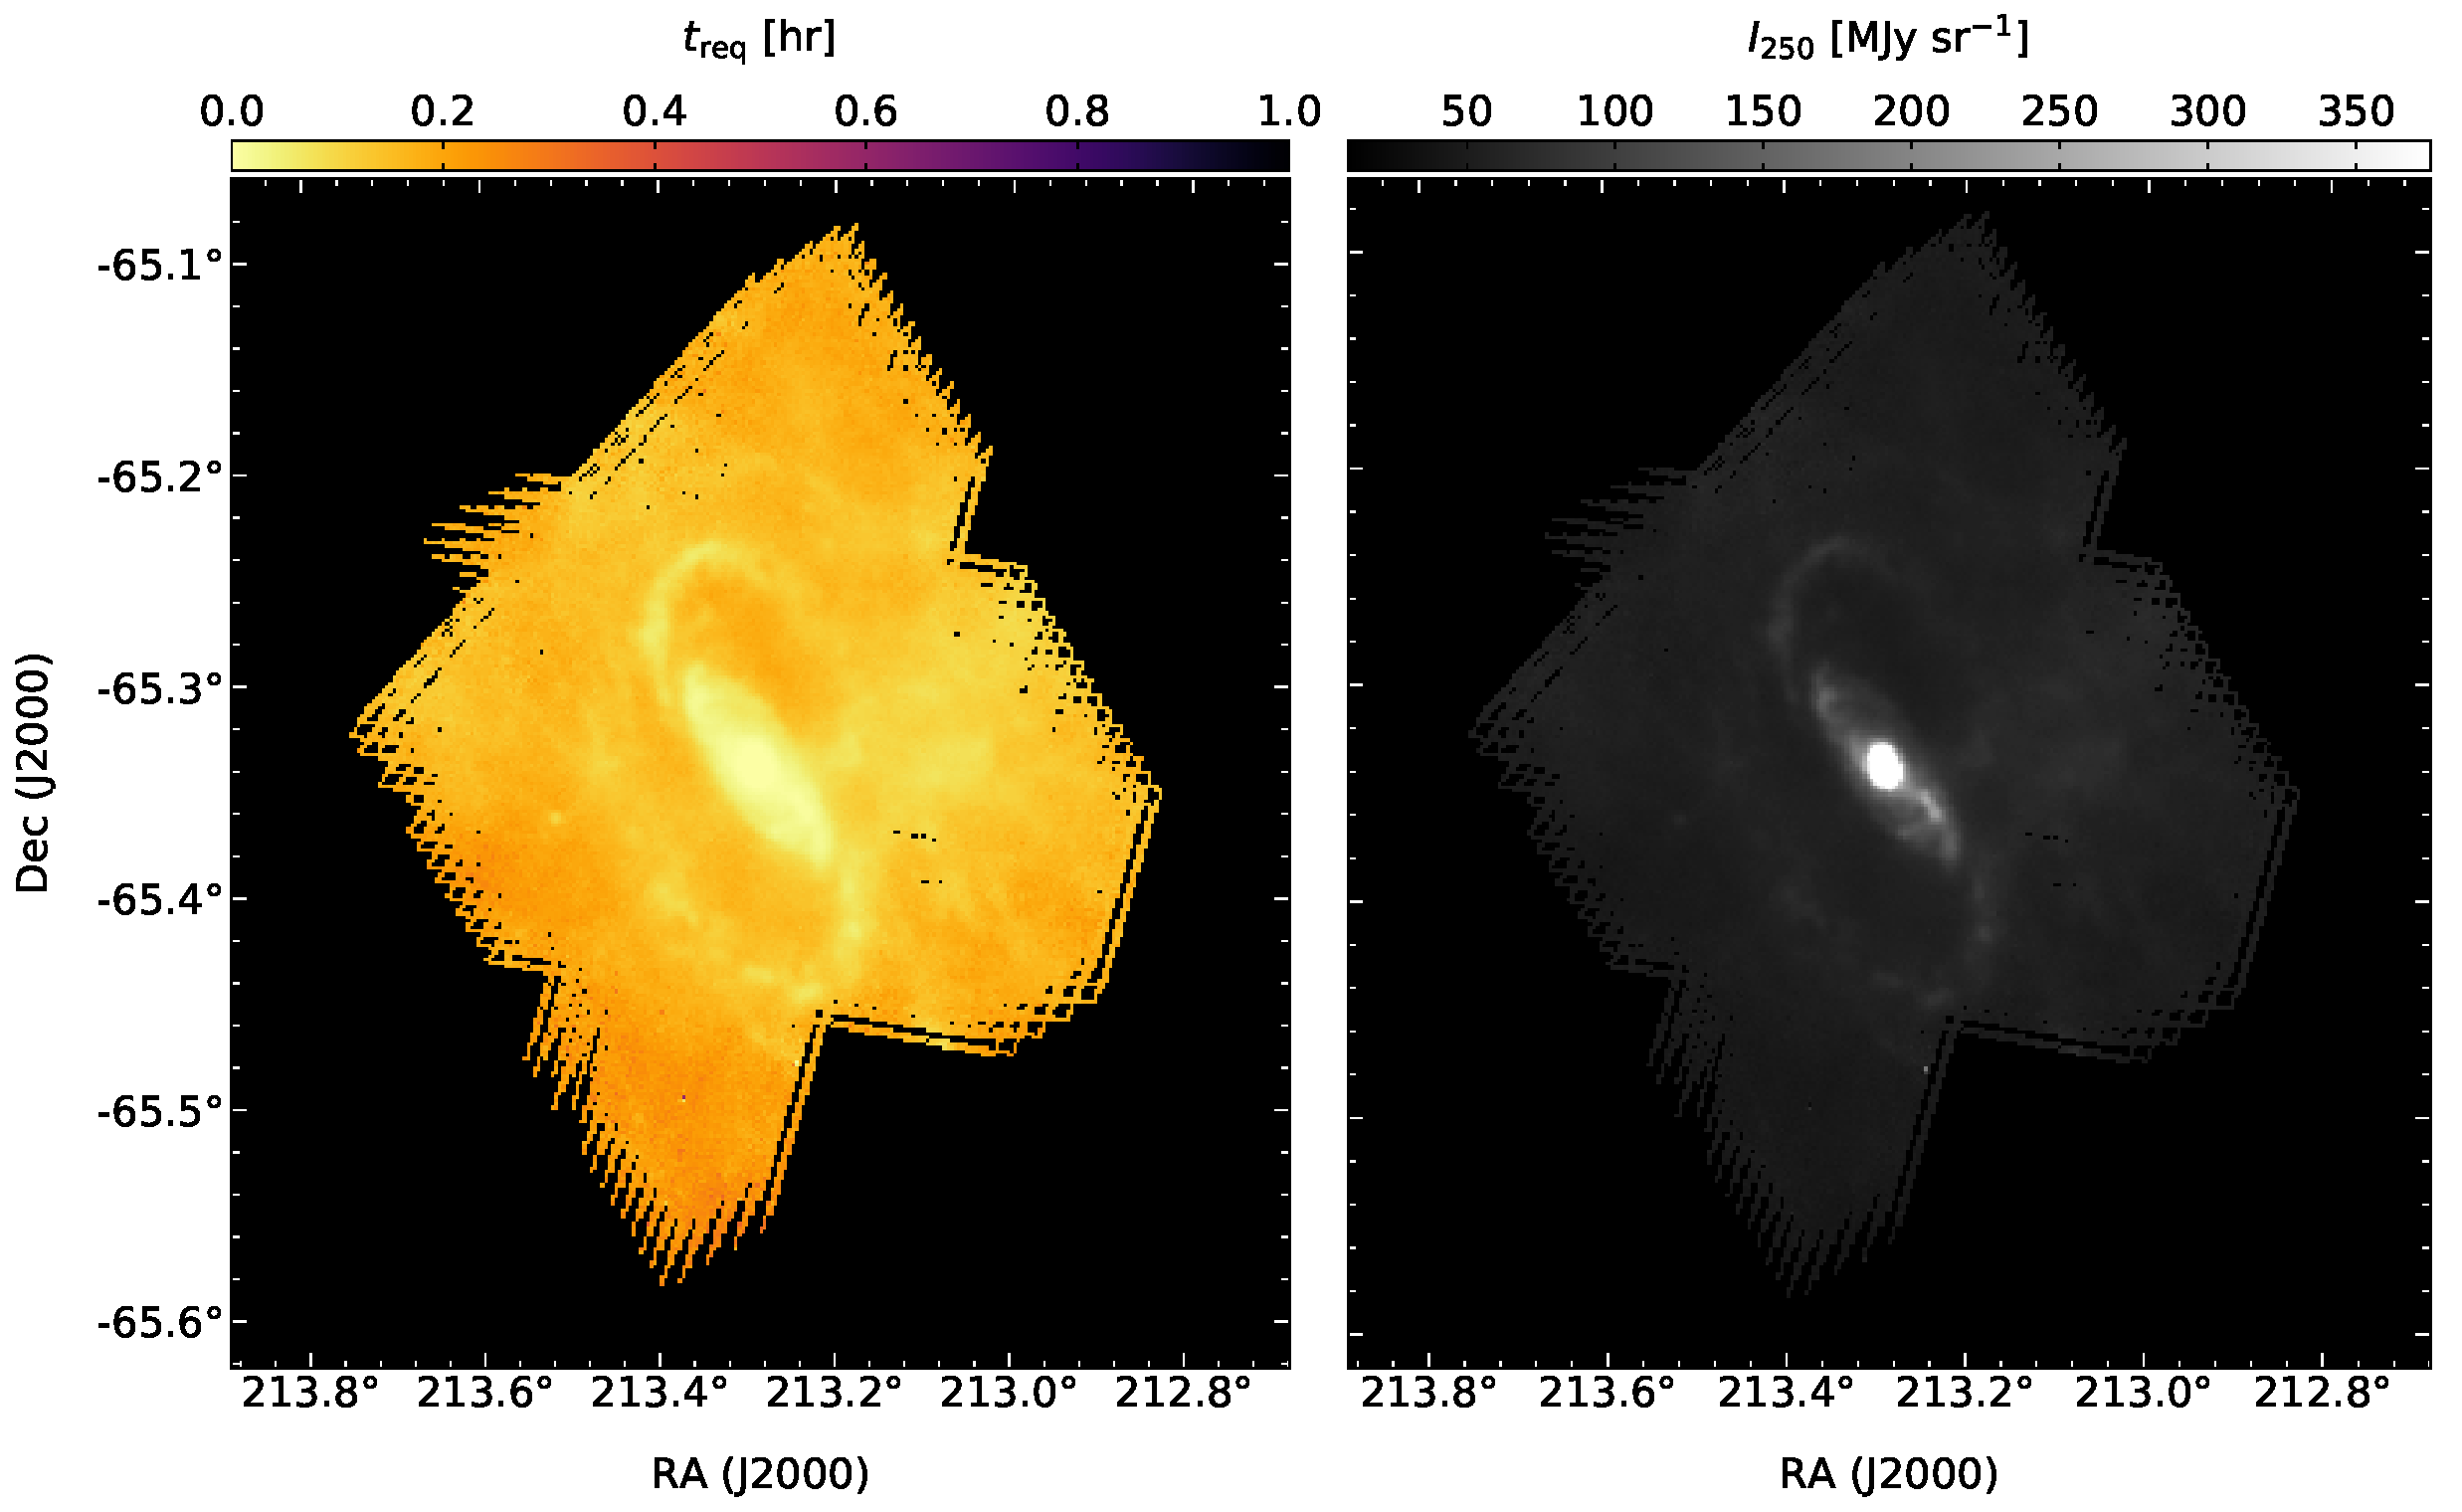
\includegraphics[scale=0.35]{figures/carina/eso9713}
\caption[ESO 97-G13.]{ESO 97-G13, images from Herschel 250~$\upmu$m.}
\label{fig:eso9713}
\end{figure}

\begin{figure}[!htbp]
\centering
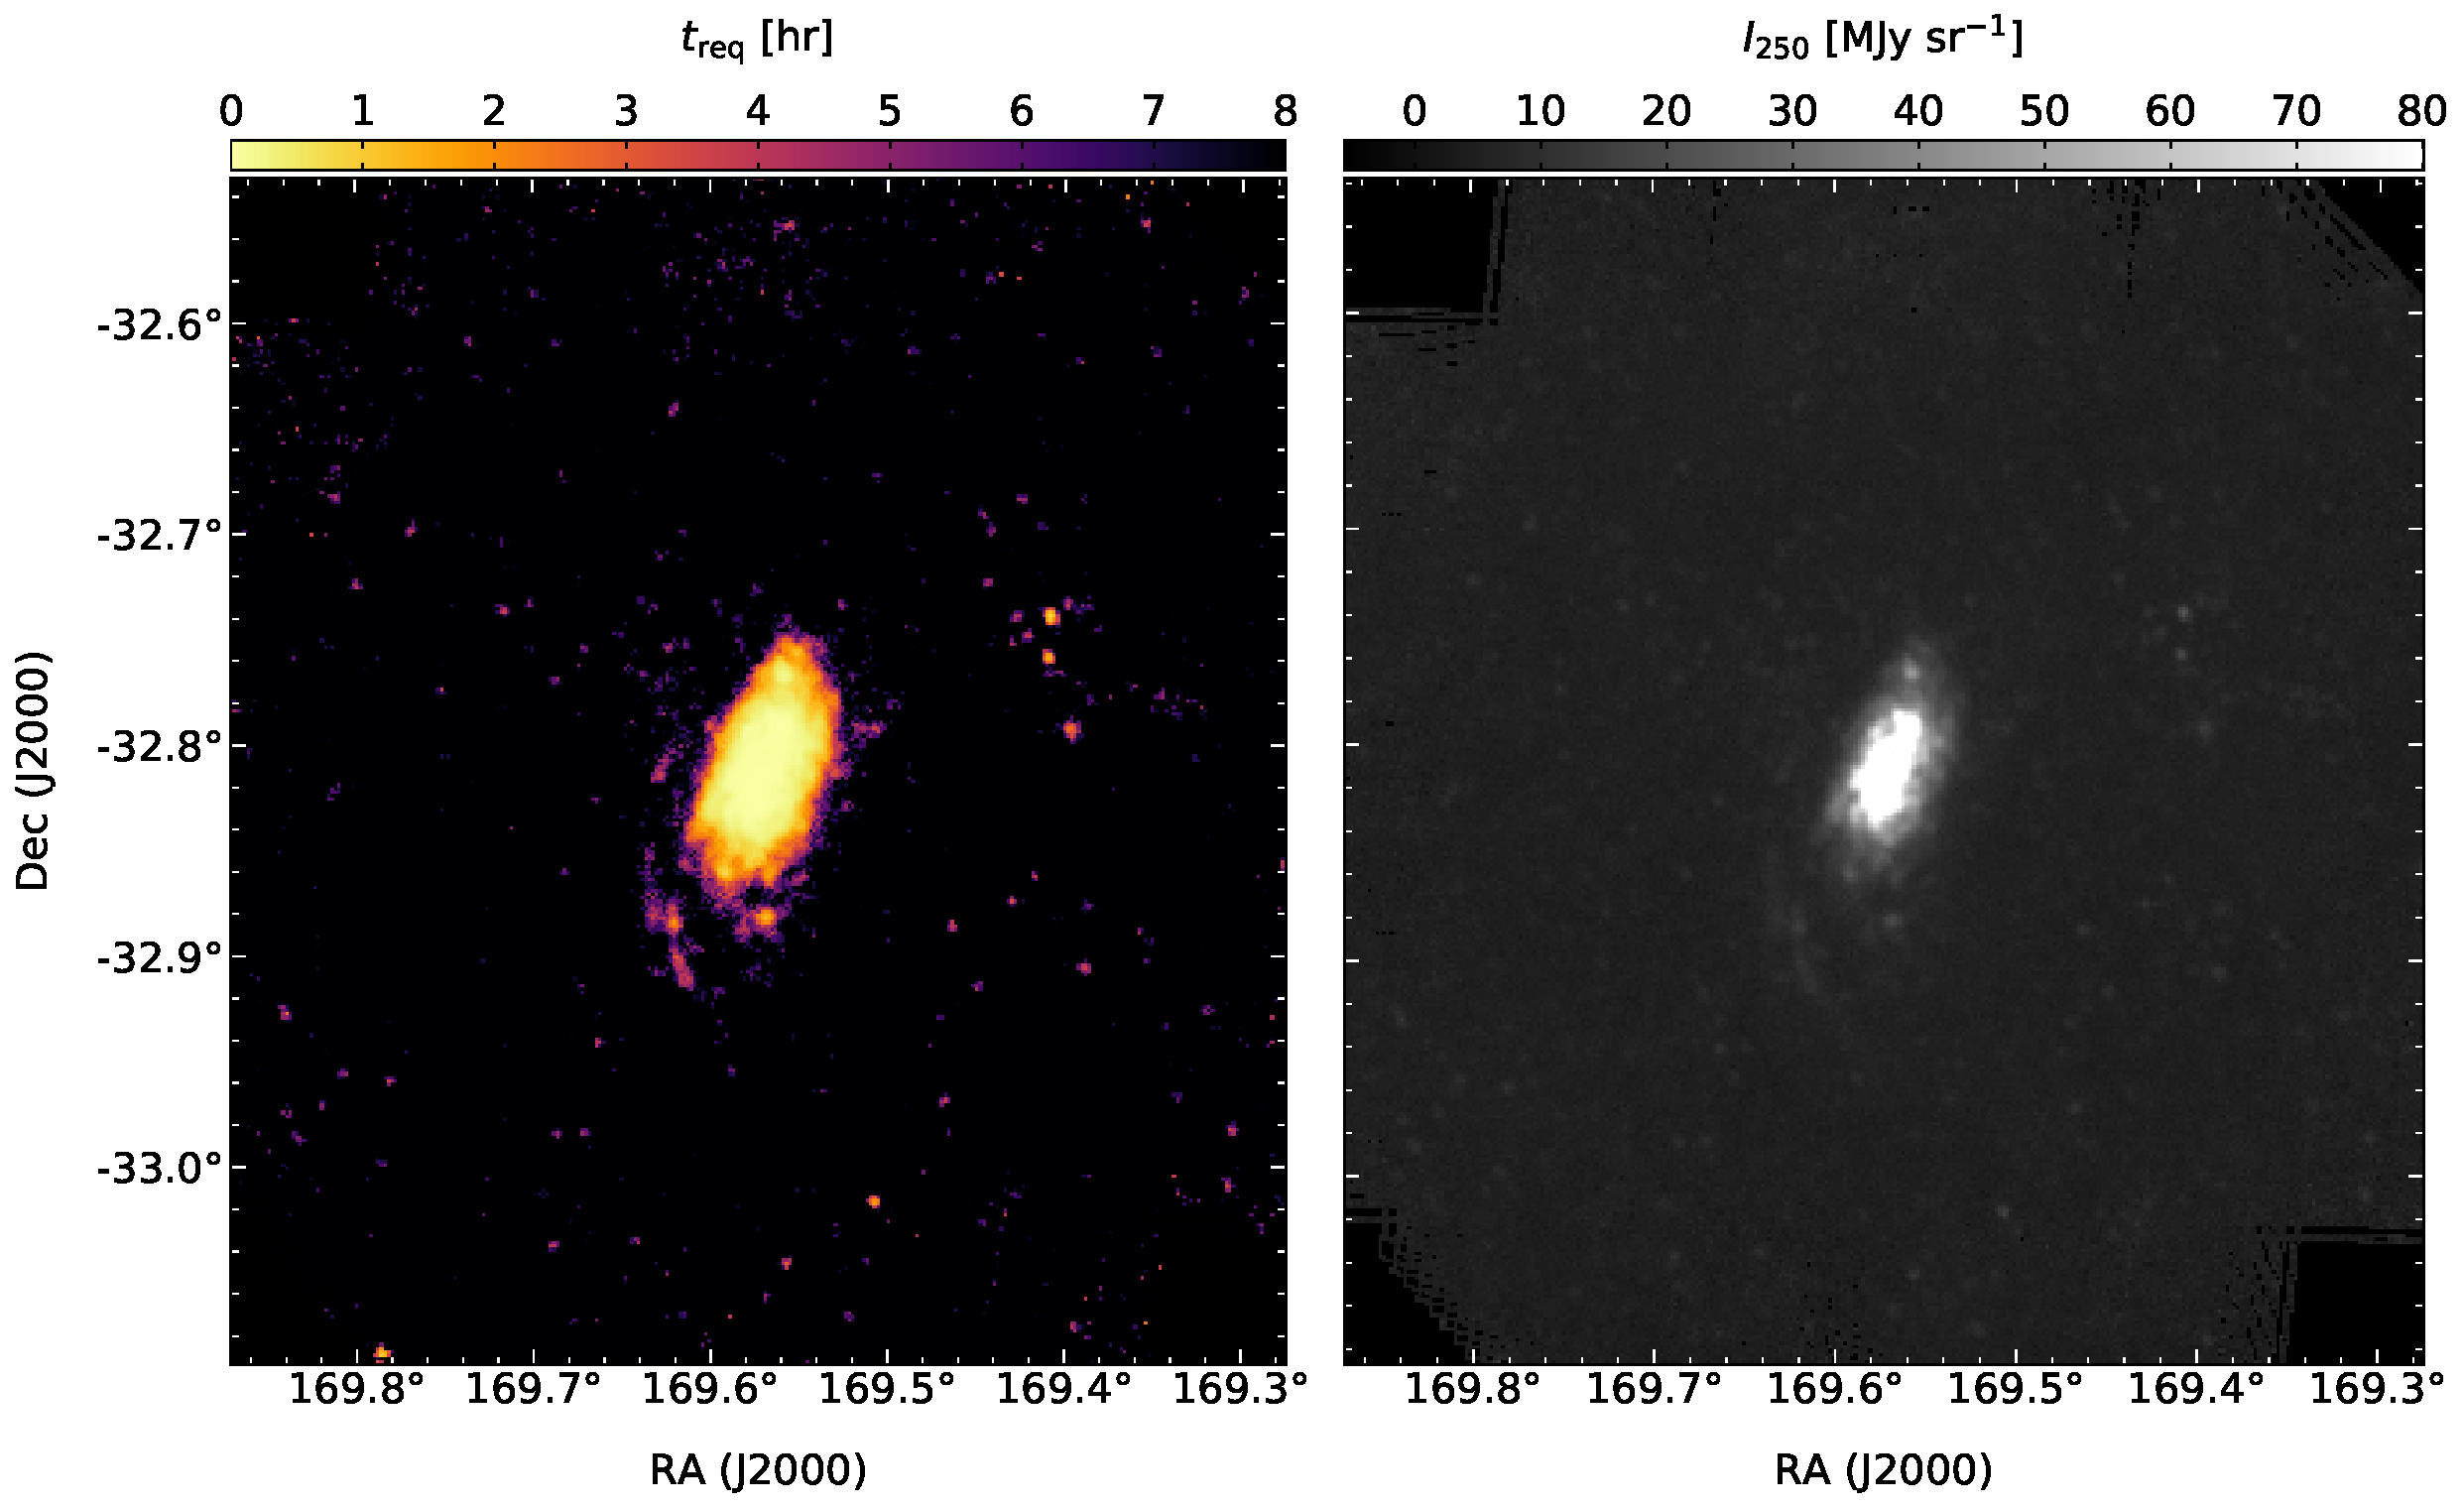
\includegraphics[scale=0.35]{figures/carina/ngc3621}
\caption[NGC 3621.]{NGC 3621, images from Herschel 250~$\upmu$m.}
\label{fig:ngc3621}
\end{figure}

\begin{figure}[!htbp]
\centering
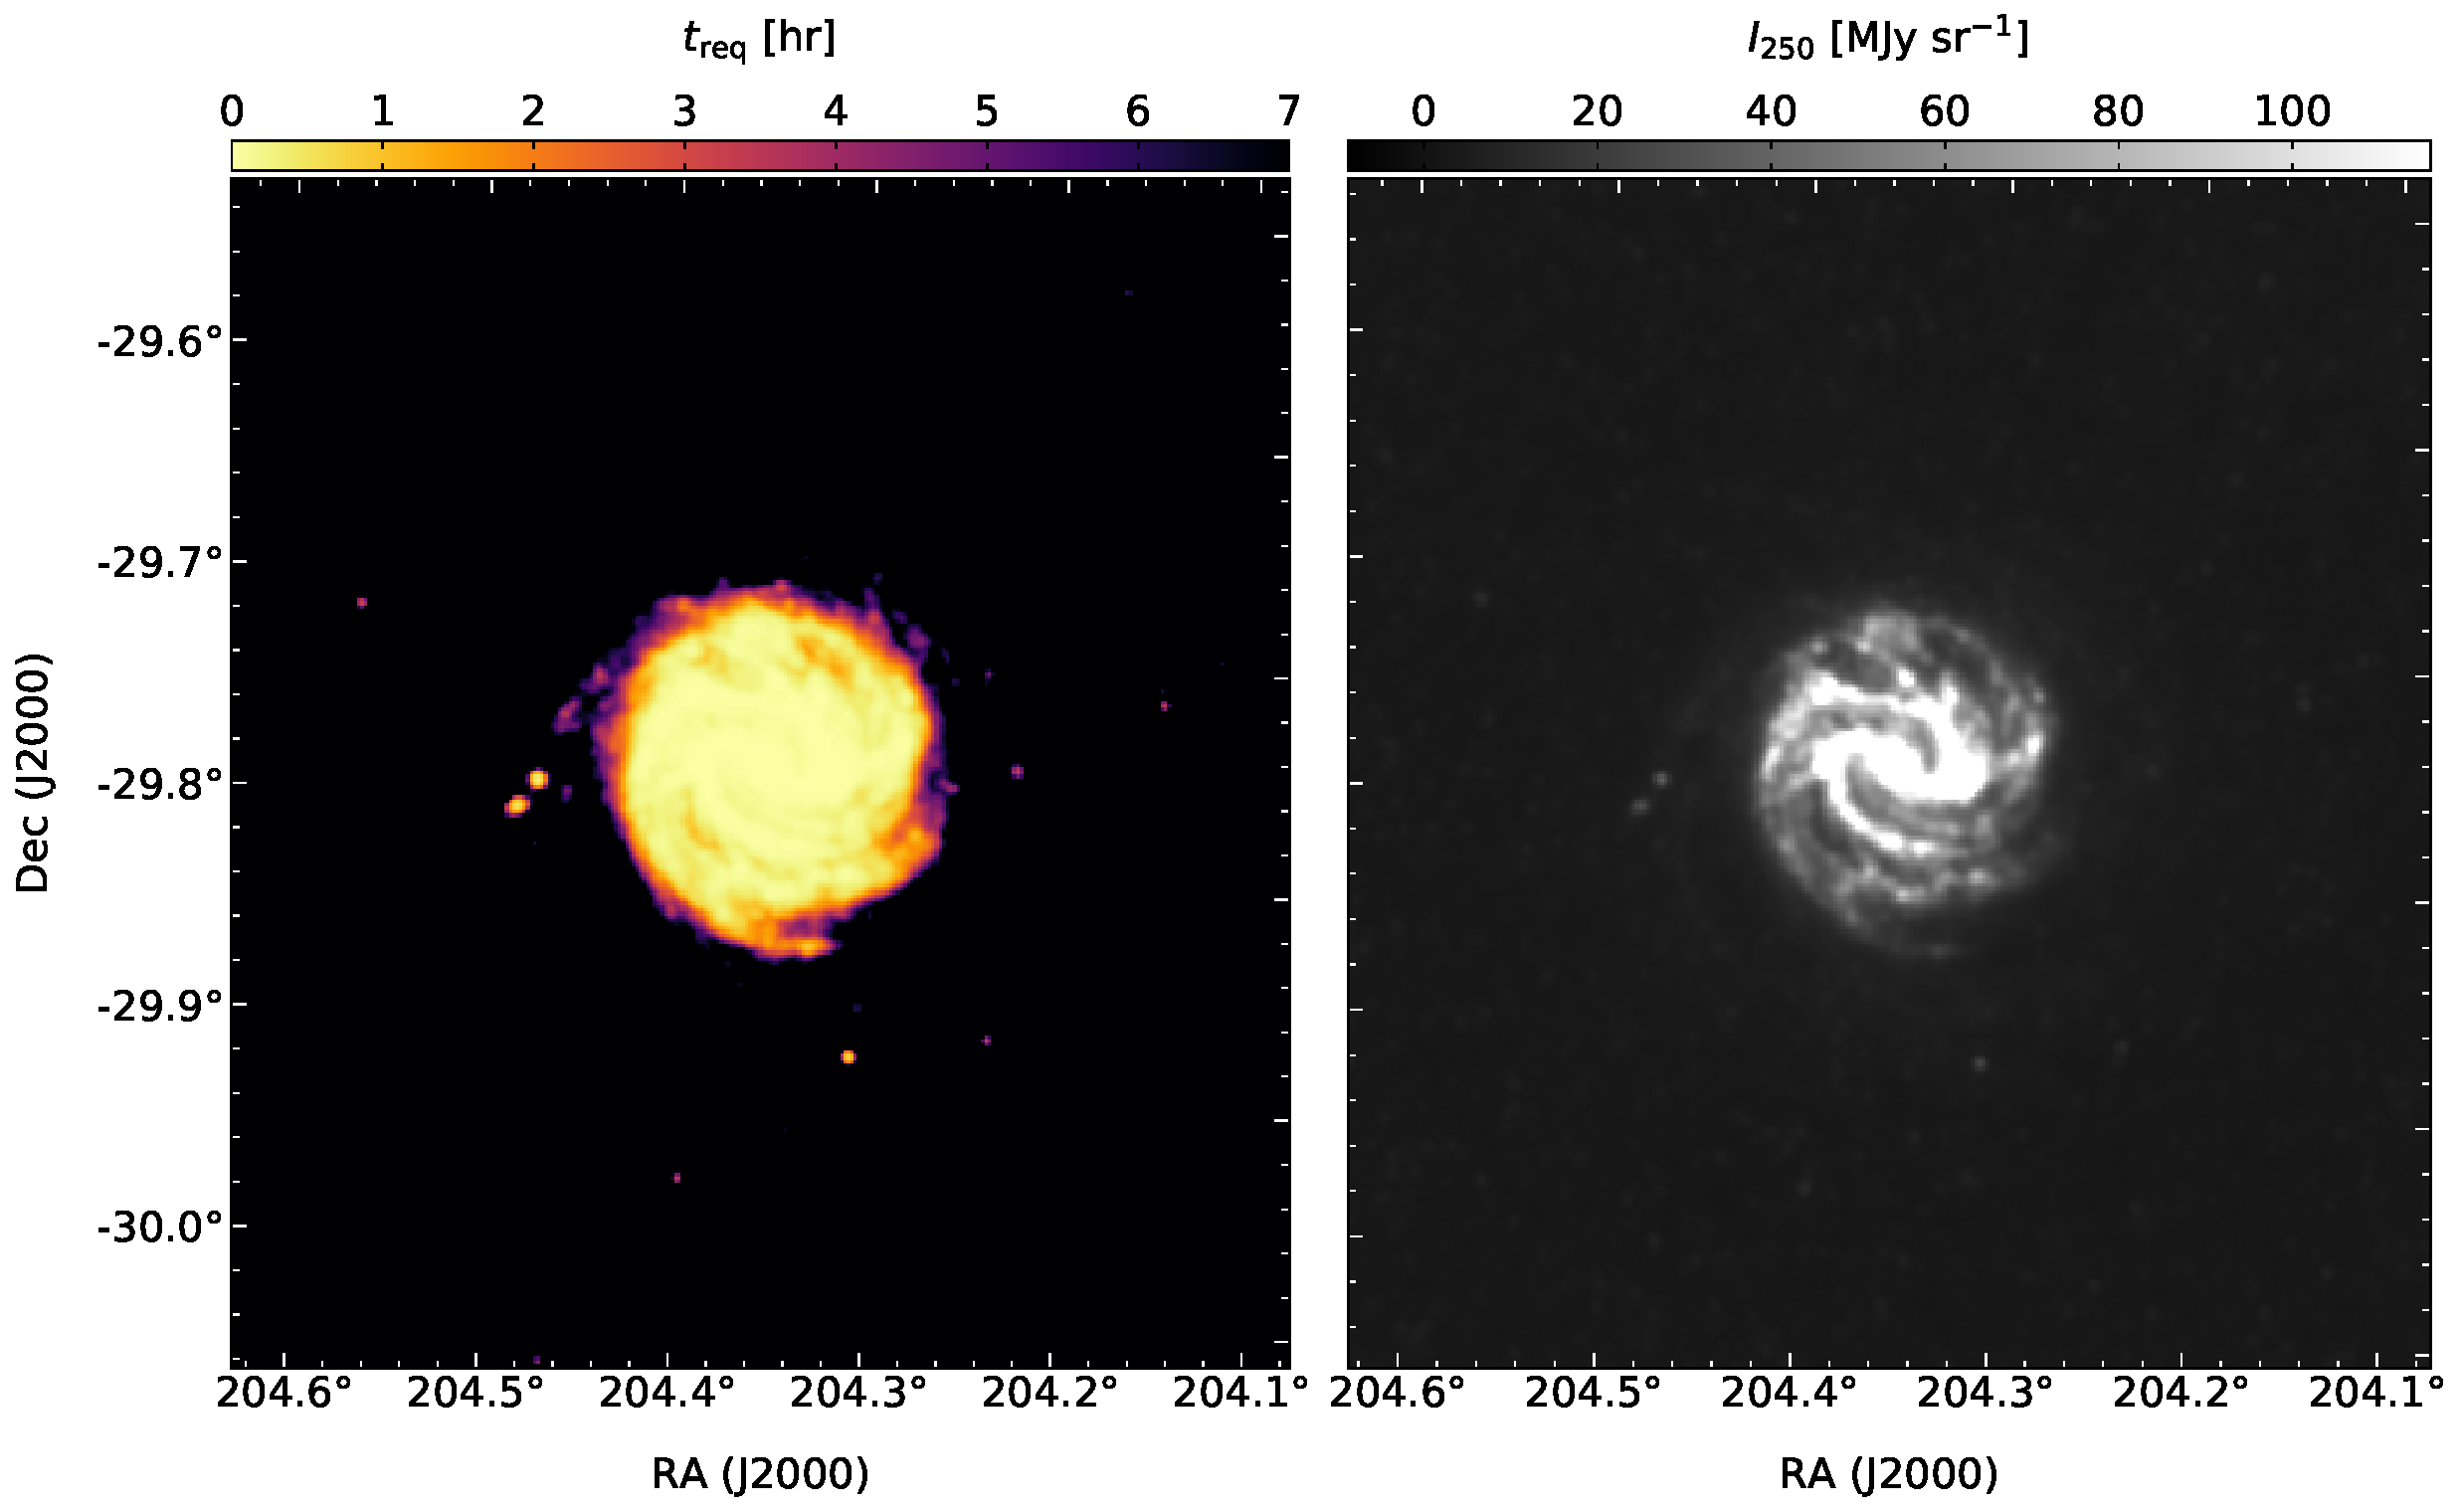
\includegraphics[scale=0.35]{figures/carina/m83}
\caption[M83.]{M83, images from Herschel 250~$\upmu$m.}
\label{fig:m83}
\end{figure}

\begin{figure}[!htbp]
\centering
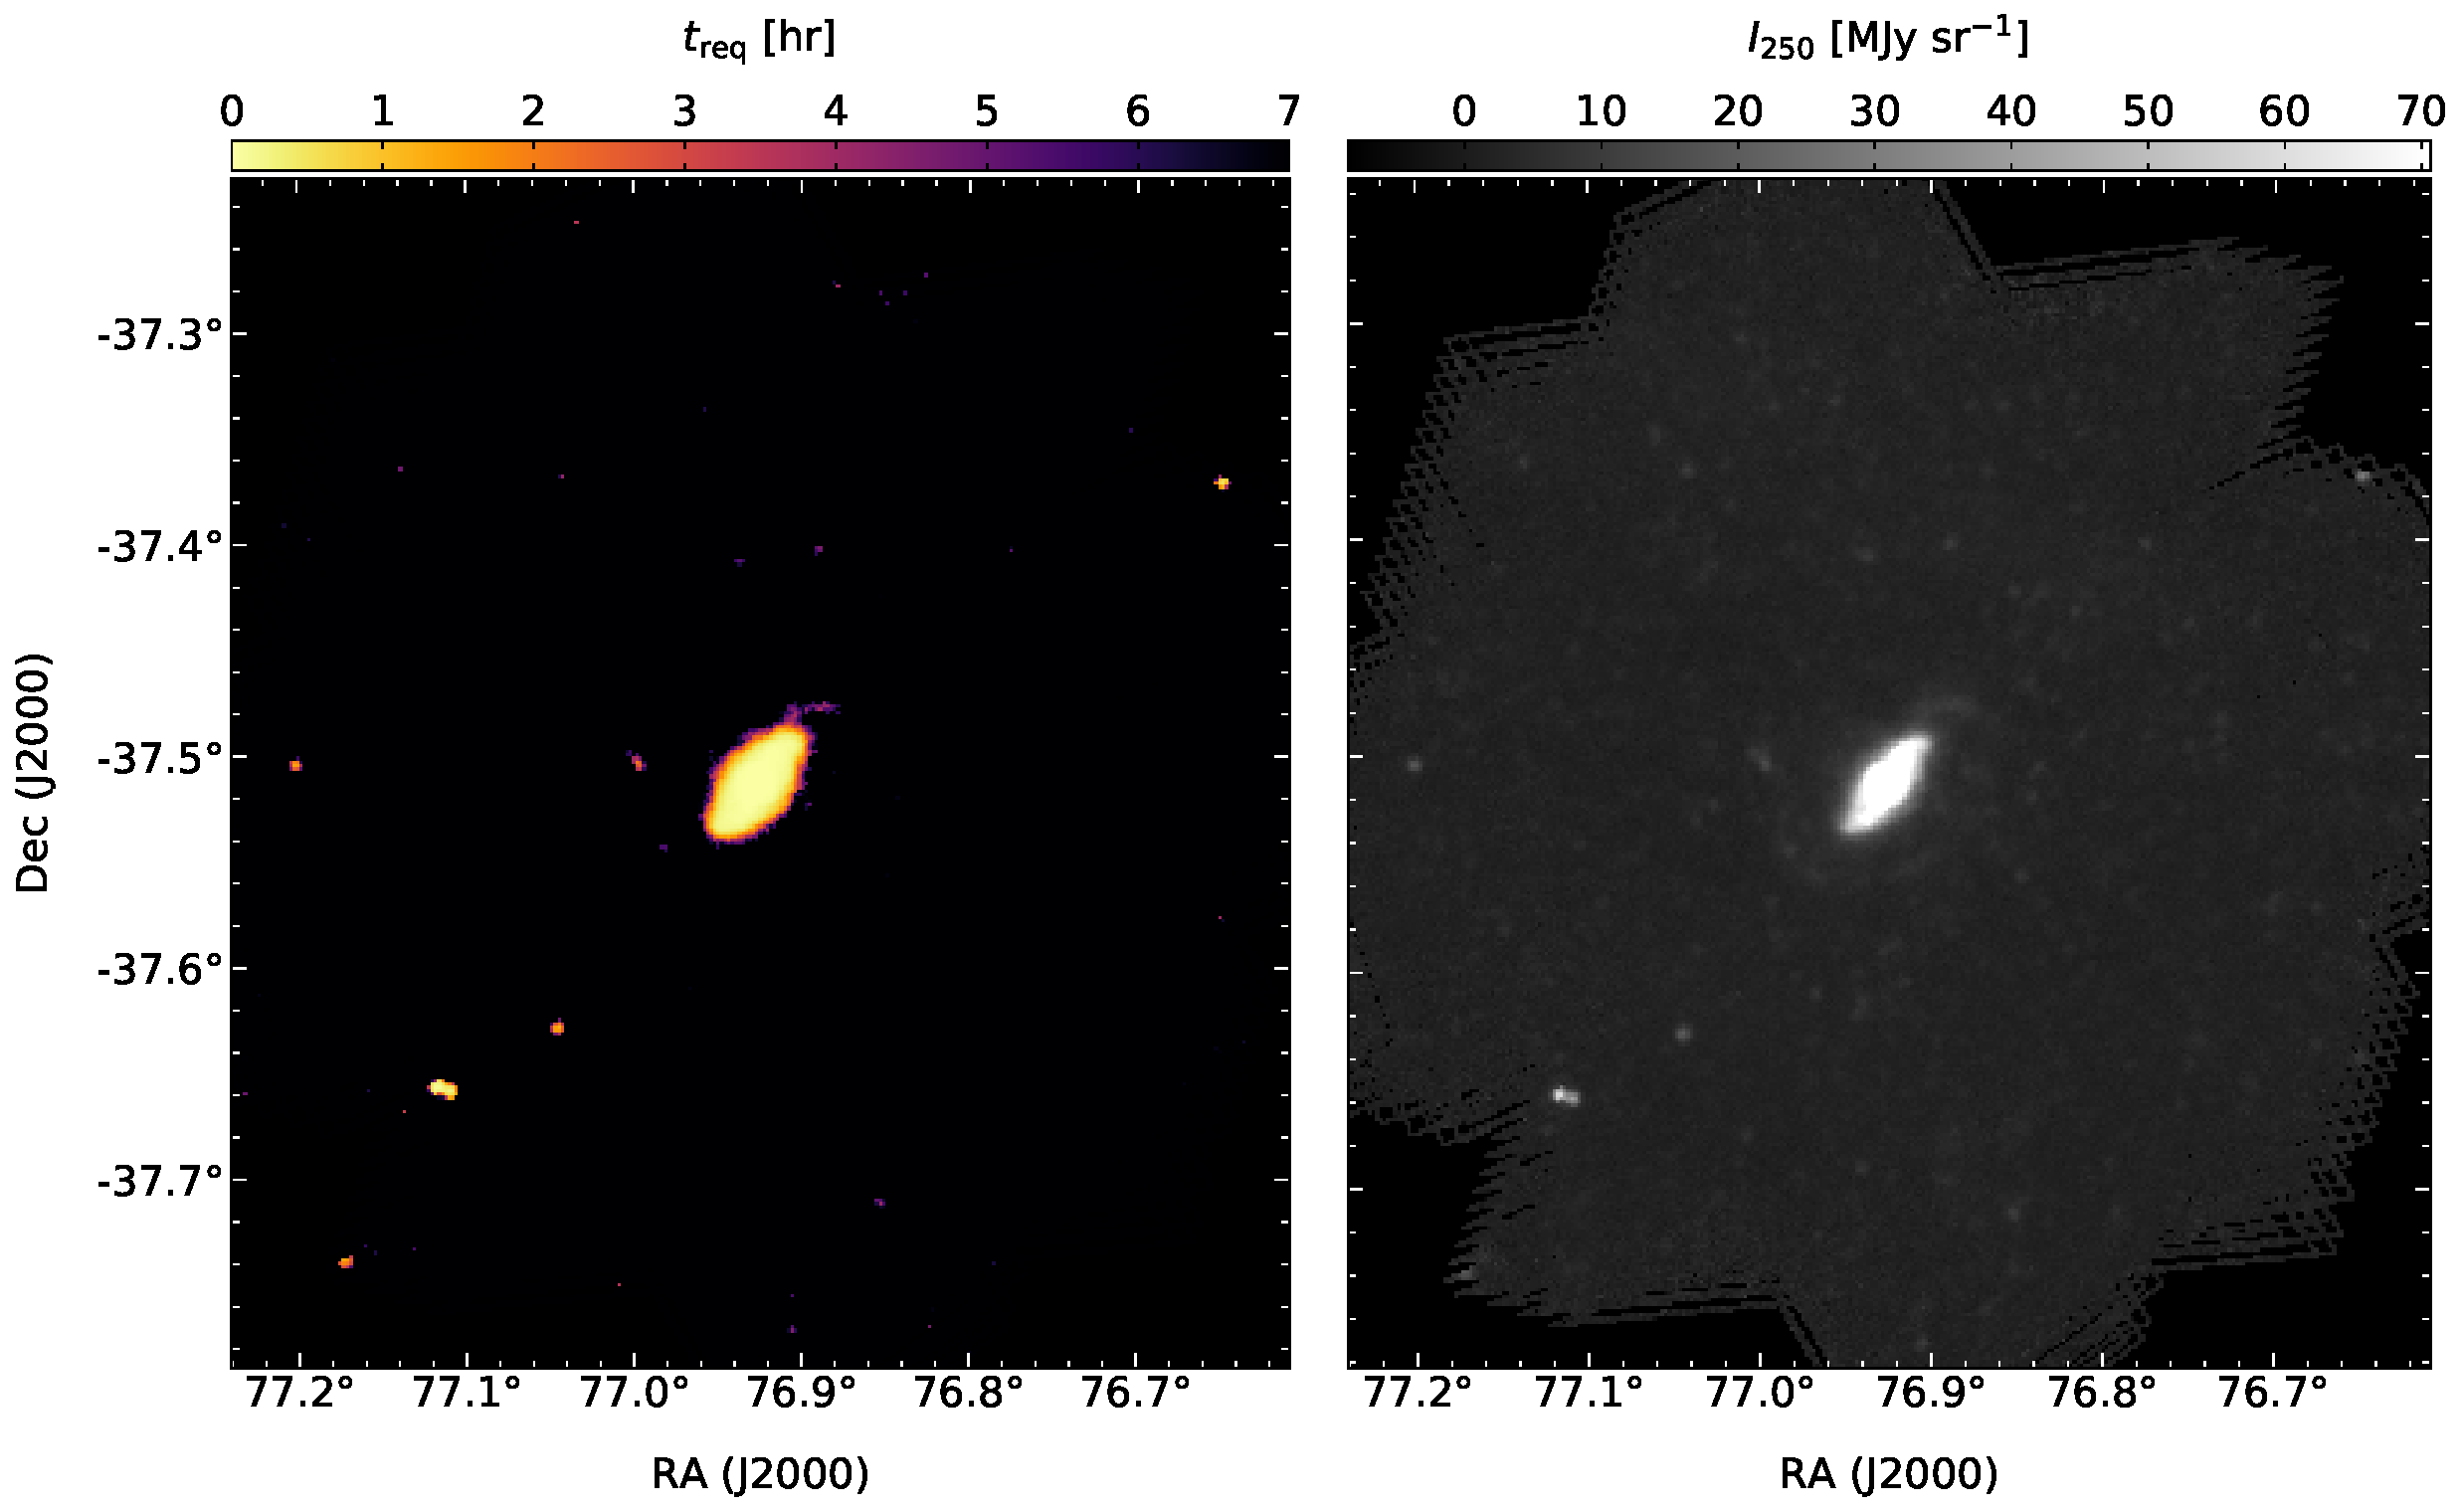
\includegraphics[scale=0.35]{figures/carina/ngc1808}
\caption[NGC 1808.]{NGC 1808, images from Herschel 250~$\upmu$m.}
\label{fig:ngc1808}
\end{figure}

\end{comment}
